\subsection{Plots for Cancer Model with \(\epsilon = 0.01\) (\cref{exp:1})}\label{sec:rescancer0.01}
\begin{figure}[H]
  \includegraphics[width=\textwidth]{plots_v2/Cancer/eps=0.01/plot_ptas-d-d.pdf}
  \caption{Features distrusted and labels distrusted}
\end{figure}
\begin{figure}[H]
  \includegraphics[width=\textwidth]{plots_v2/Cancer/eps=0.01/plot_ptas-d-v.pdf}
  \caption{Features distrusted and labels vacuous}
\end{figure}
\begin{figure}[H]
  \includegraphics[width=\textwidth]{plots_v2/Cancer/eps=0.01/plot_ptas-d-t.pdf}
  \caption{Features distrusted and labels trusted}
\end{figure}
\begin{figure}[H]
  \includegraphics[width=\textwidth]{plots_v2/Cancer/eps=0.01/plot_ptas-v-d.pdf}
  \caption{Features vacuous and labels distrusted}
\end{figure}
\begin{figure}[H]
  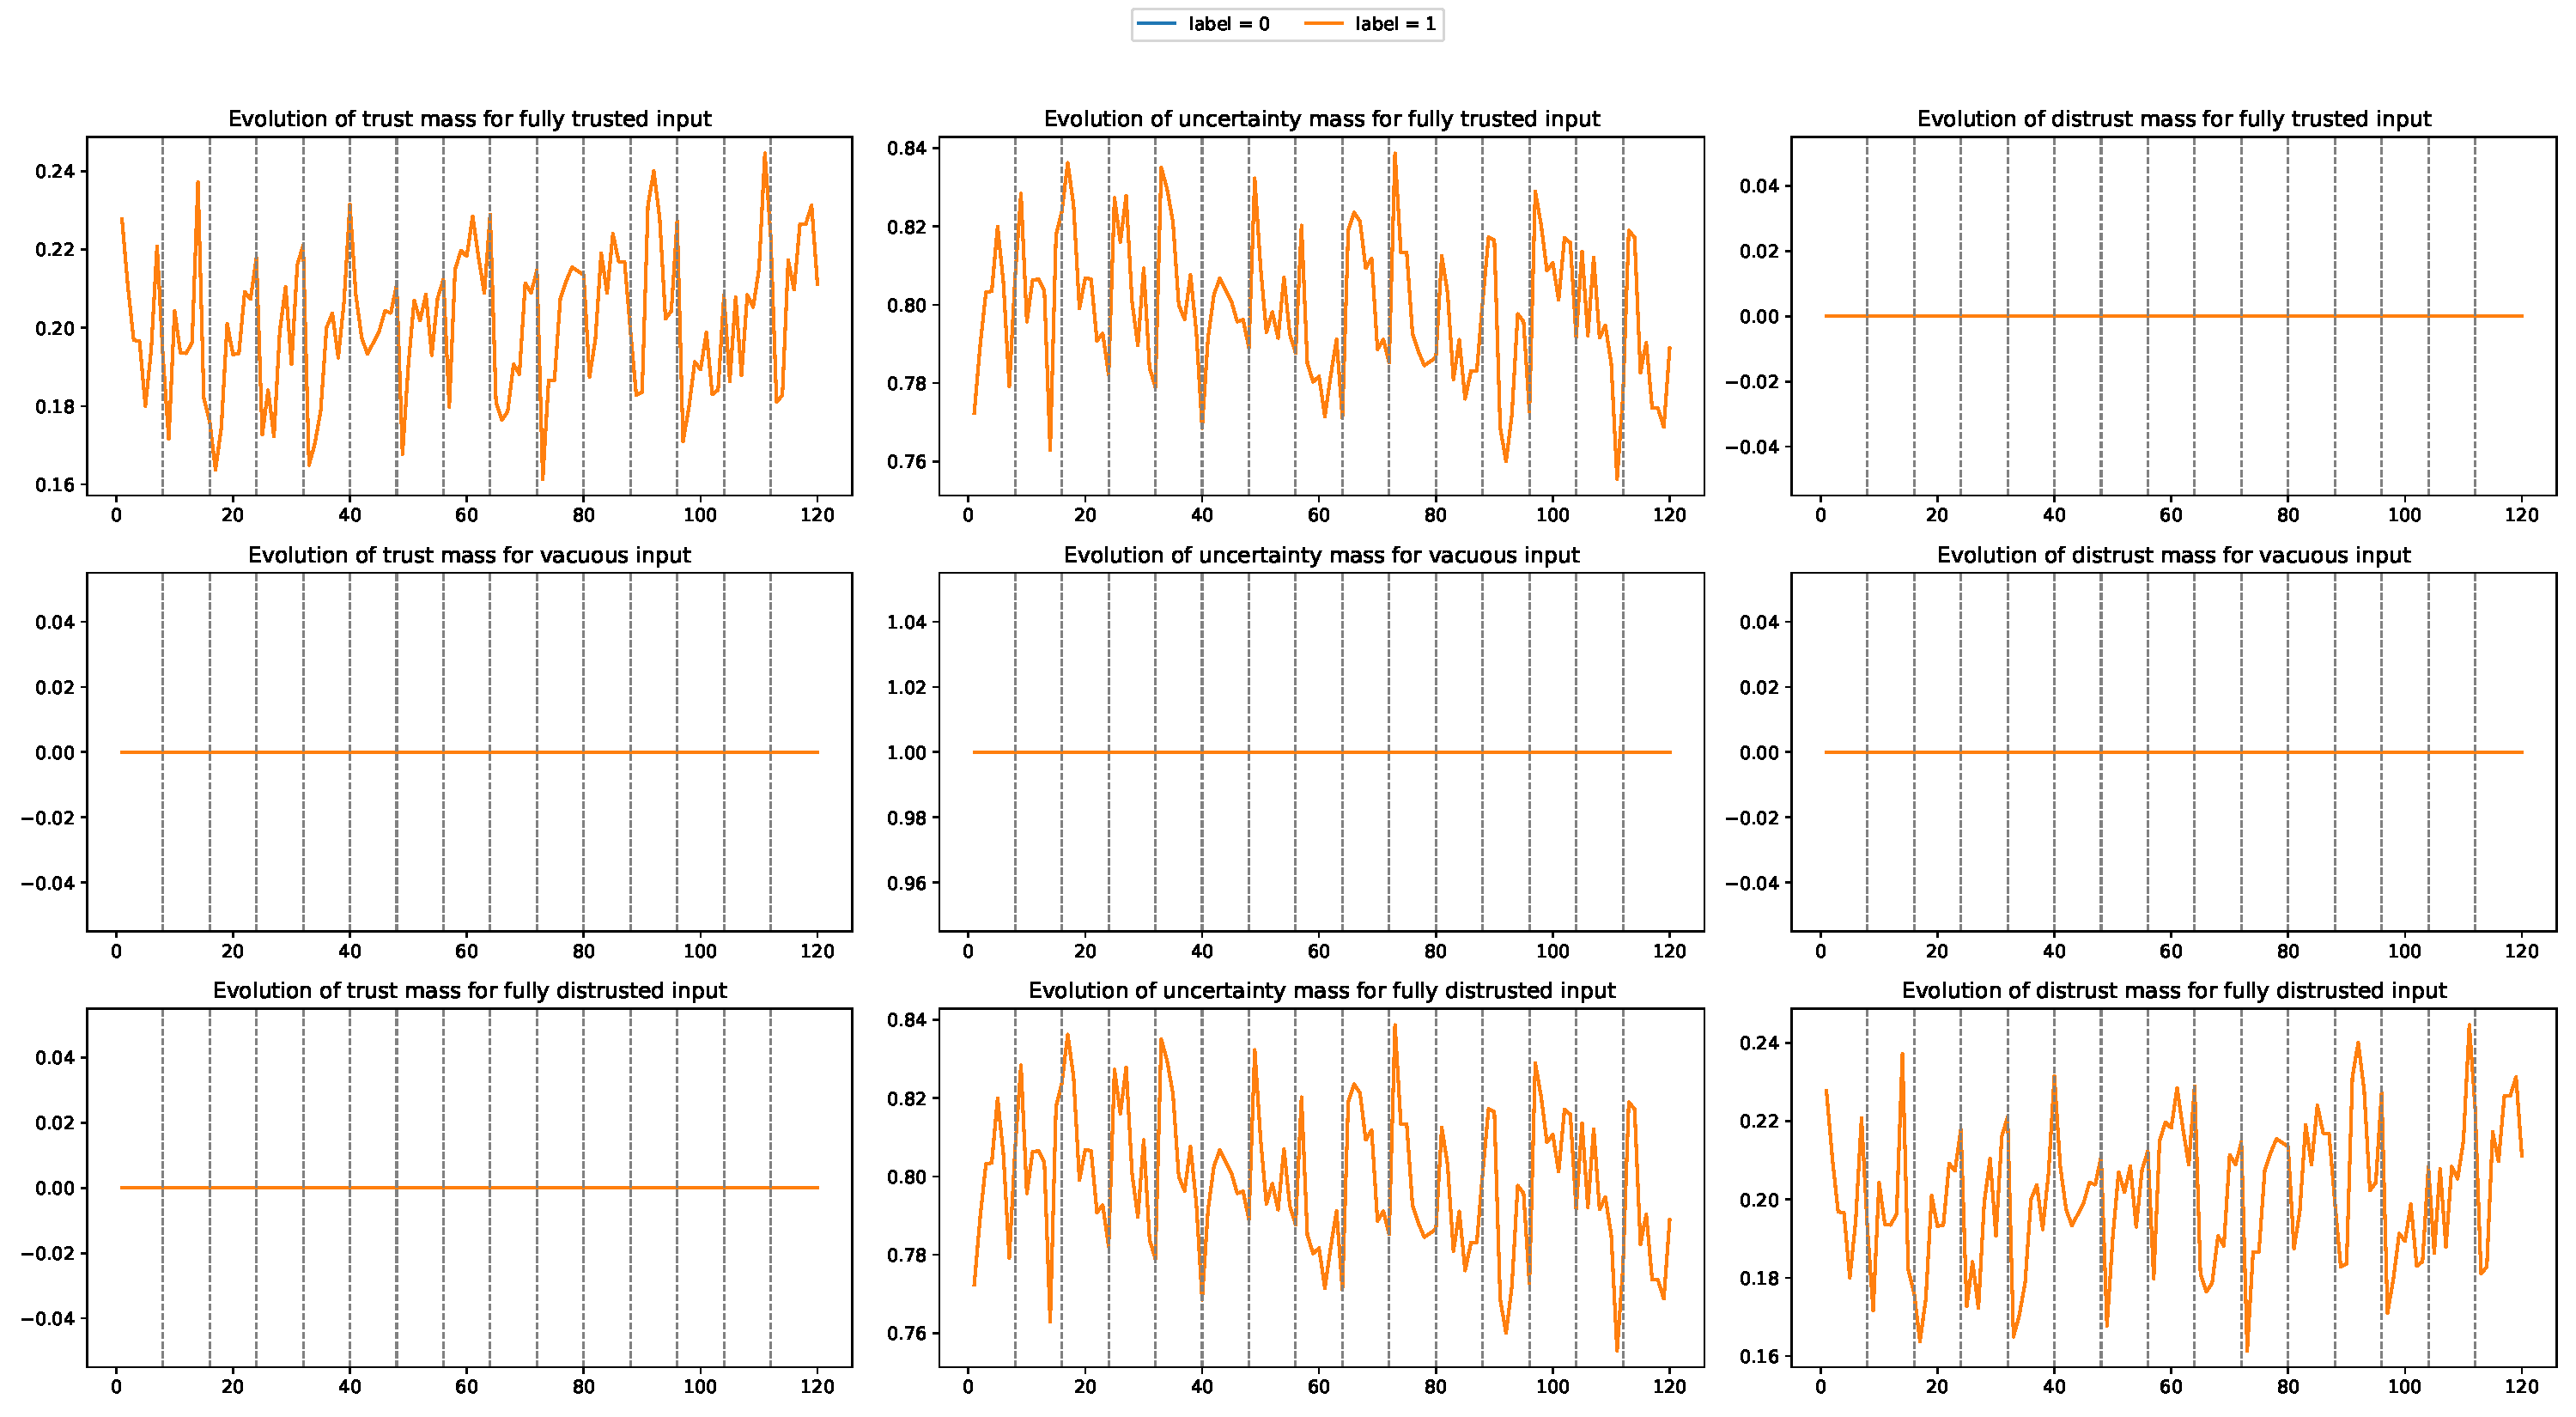
\includegraphics[width=\textwidth]{plots_v2/Cancer/eps=0.01/plot_ptas-v-v.pdf}
  \caption{Features vacuous and labels vacuous}
\end{figure}
\begin{figure}[H]
  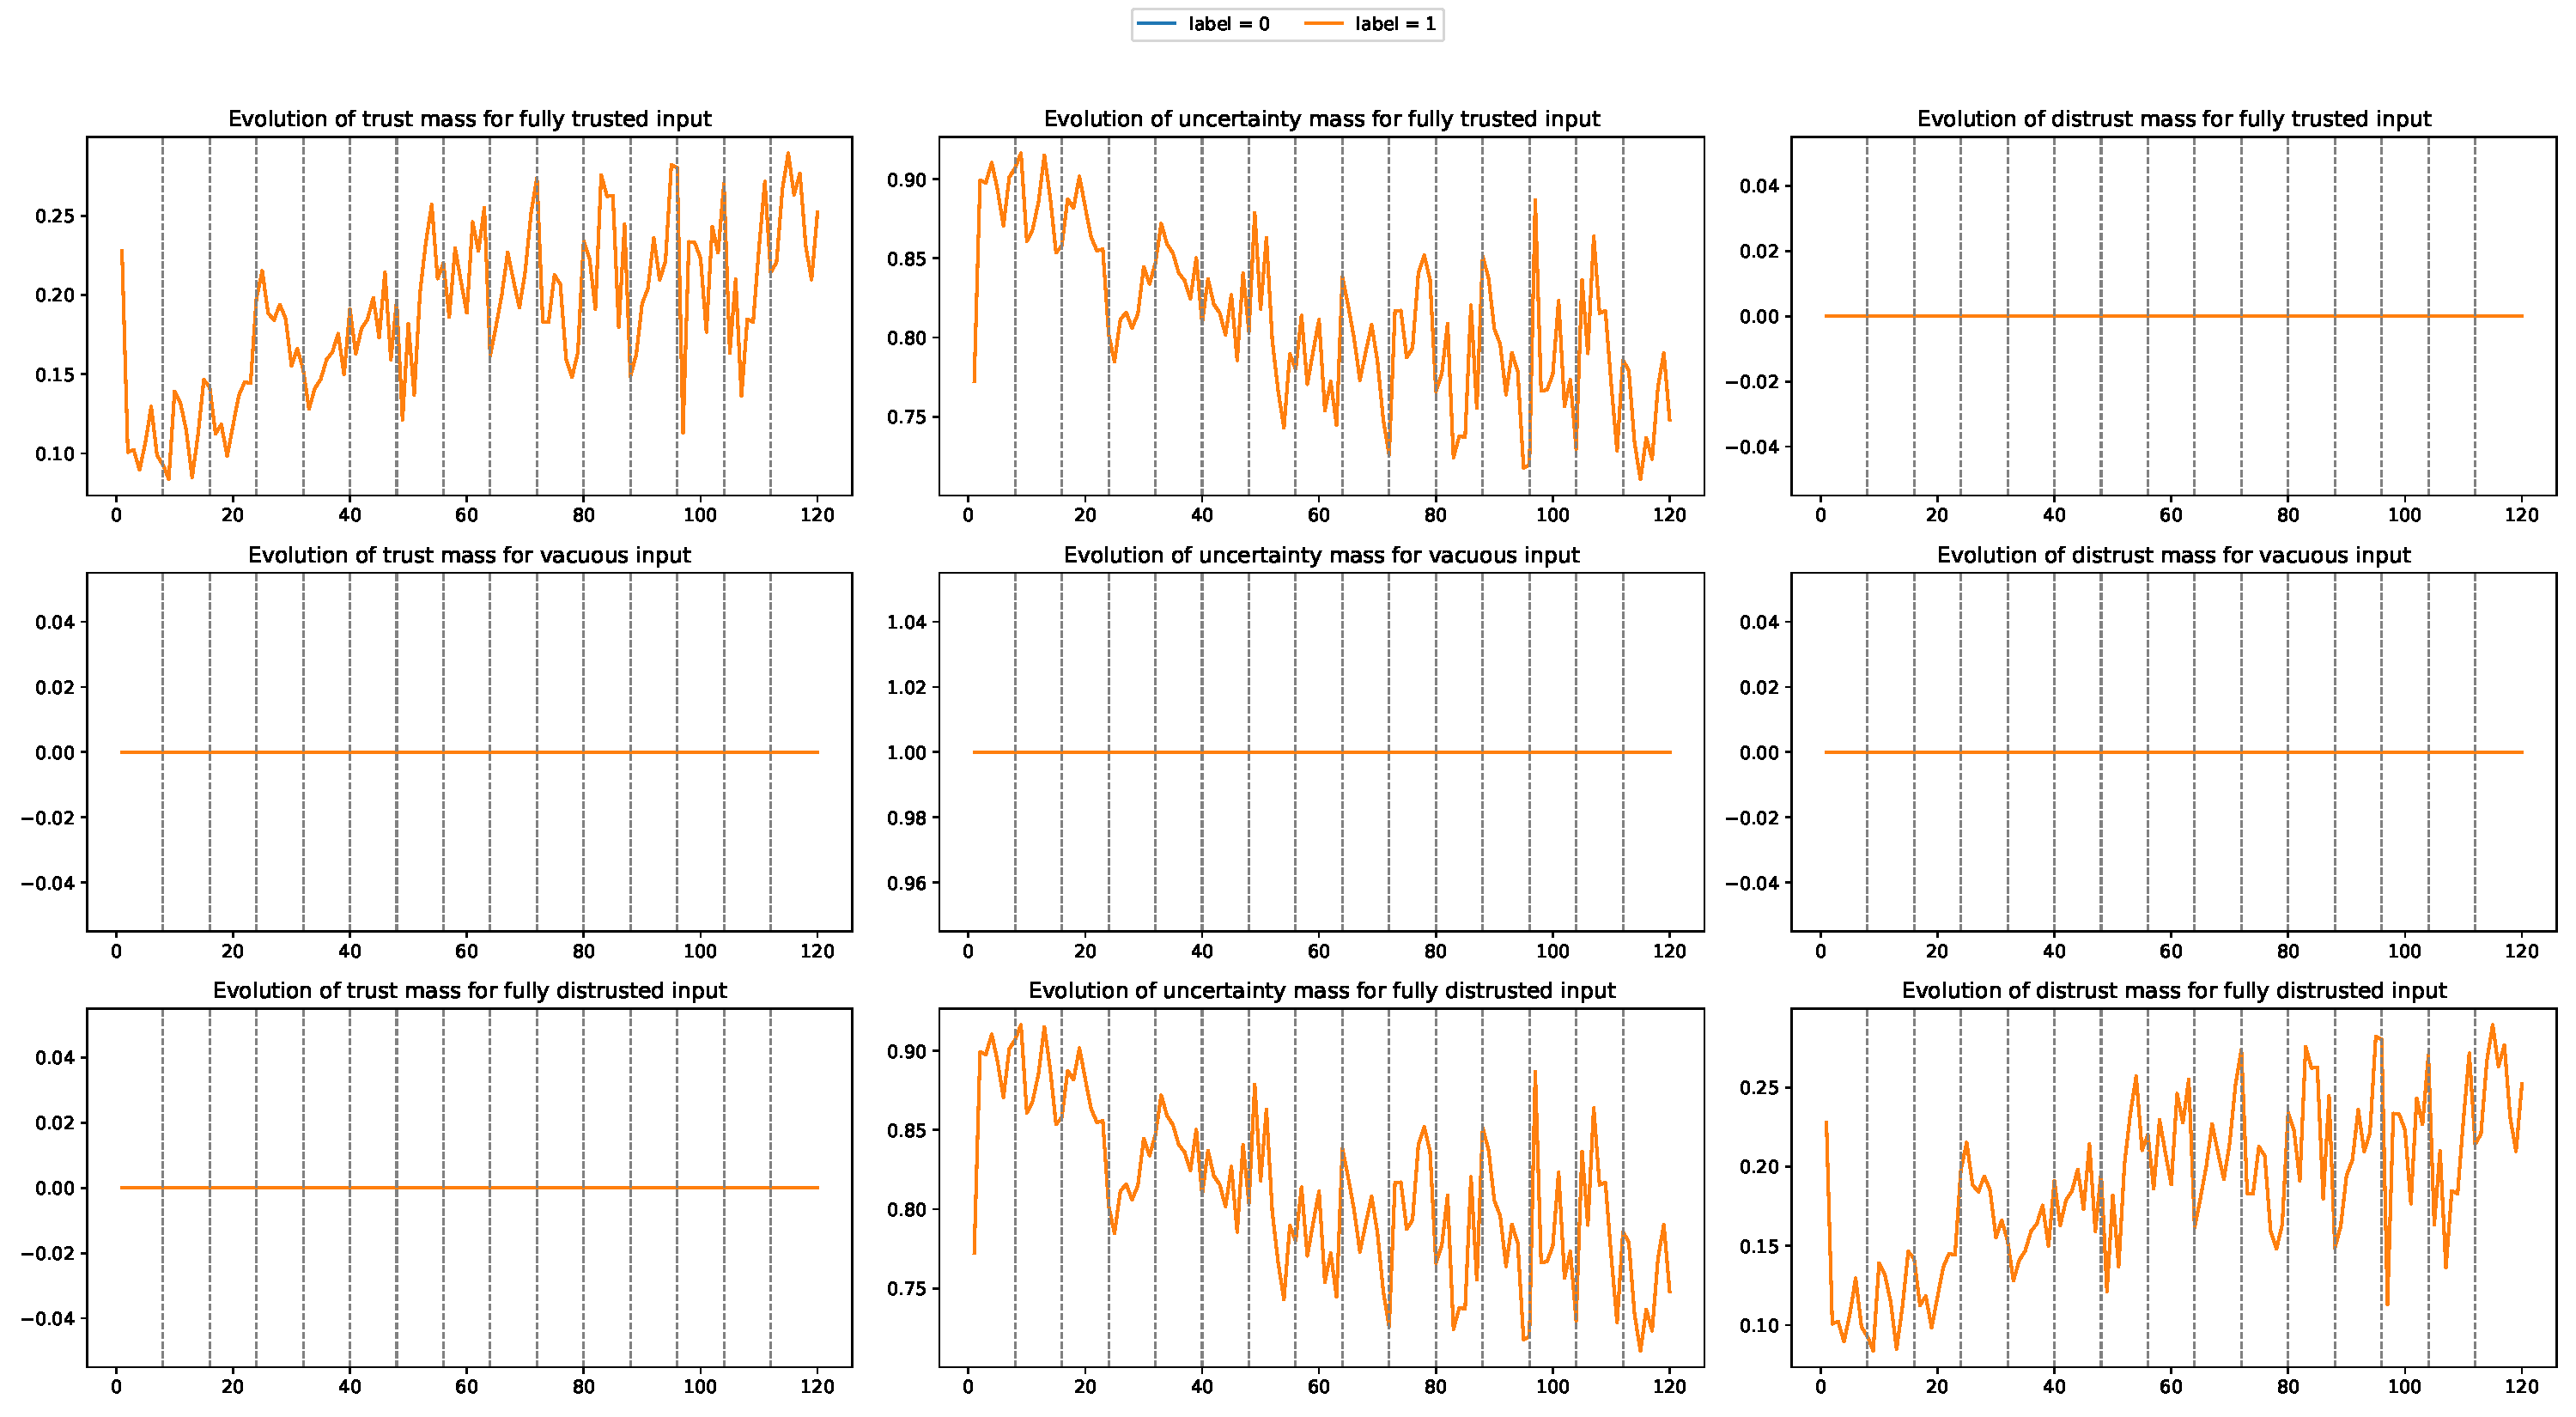
\includegraphics[width=\textwidth]{plots_v2/Cancer/eps=0.01/plot_ptas-v-t.pdf}
  \caption{Features vacuous and labels trusted}
\end{figure}
\begin{figure}[H]
  \includegraphics[width=\textwidth]{plots_v2/Cancer/eps=0.01/plot_ptas-t-d.pdf}
  \caption{Features trusted and labels distrusted}
\end{figure}
\begin{figure}[H]
  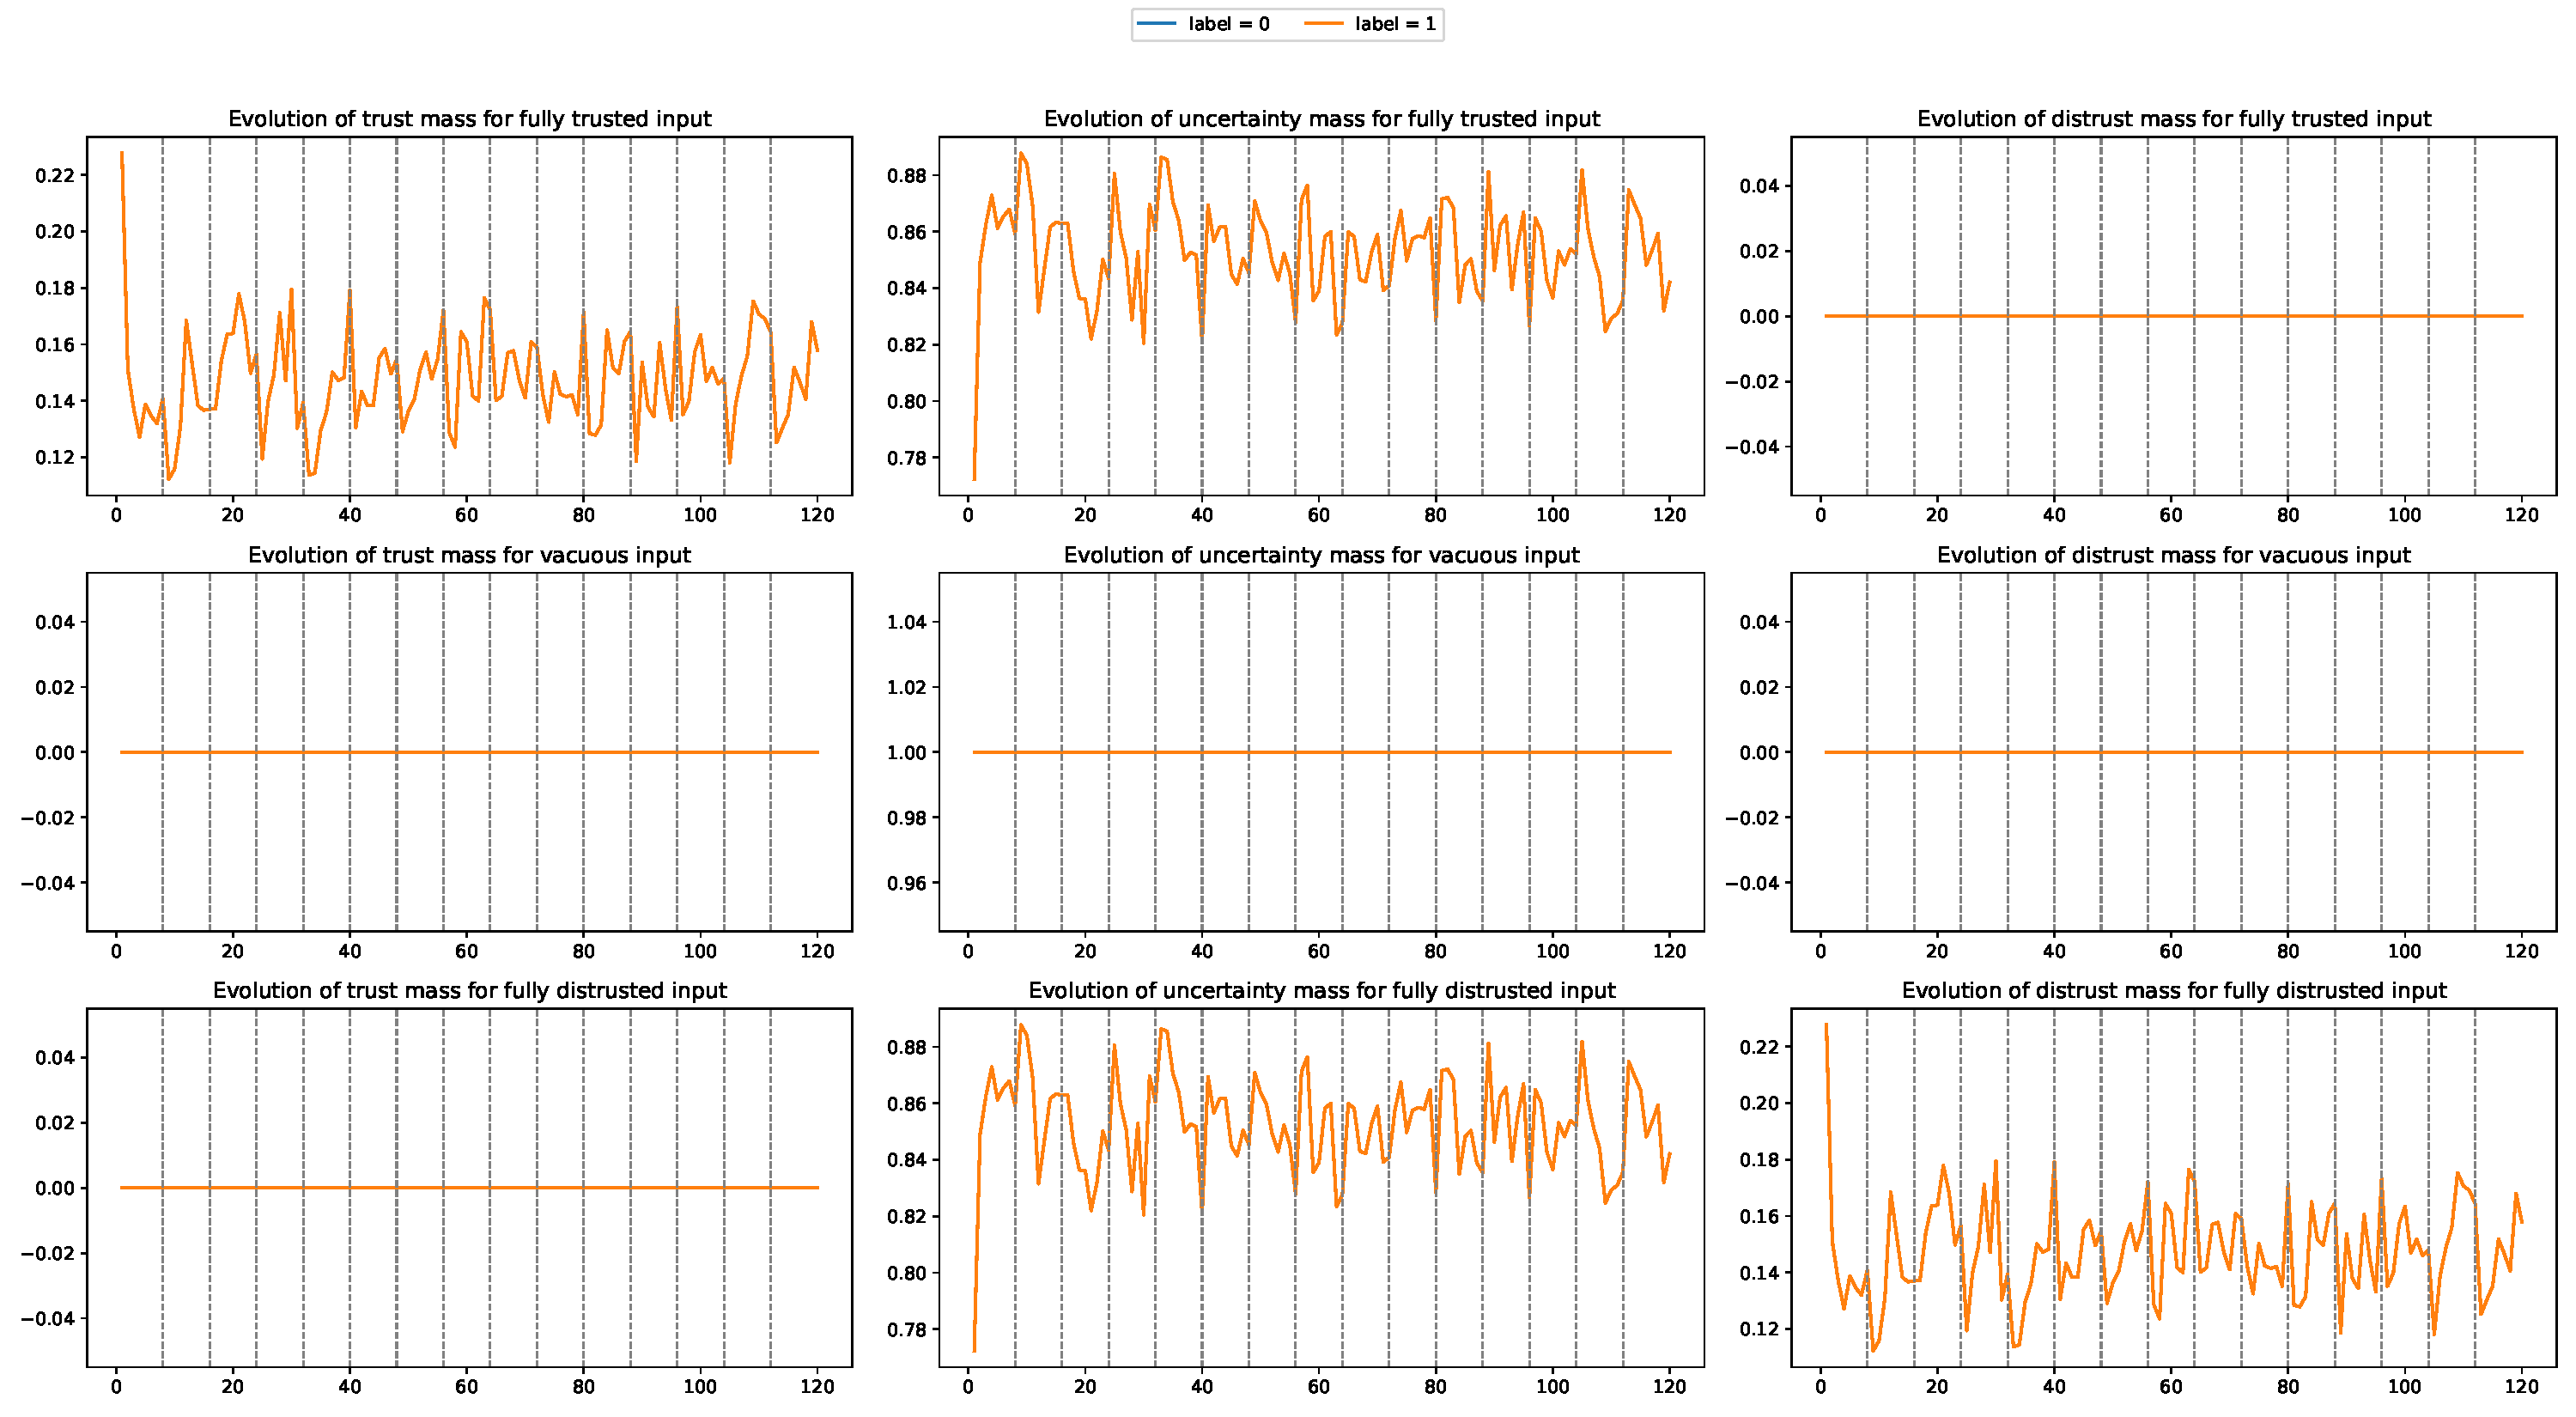
\includegraphics[width=\textwidth]{plots_v2/Cancer/eps=0.01/plot_ptas-t-v.pdf}
  \caption{Features trusted and labels vacuous}
\end{figure}
\begin{figure}[H]
  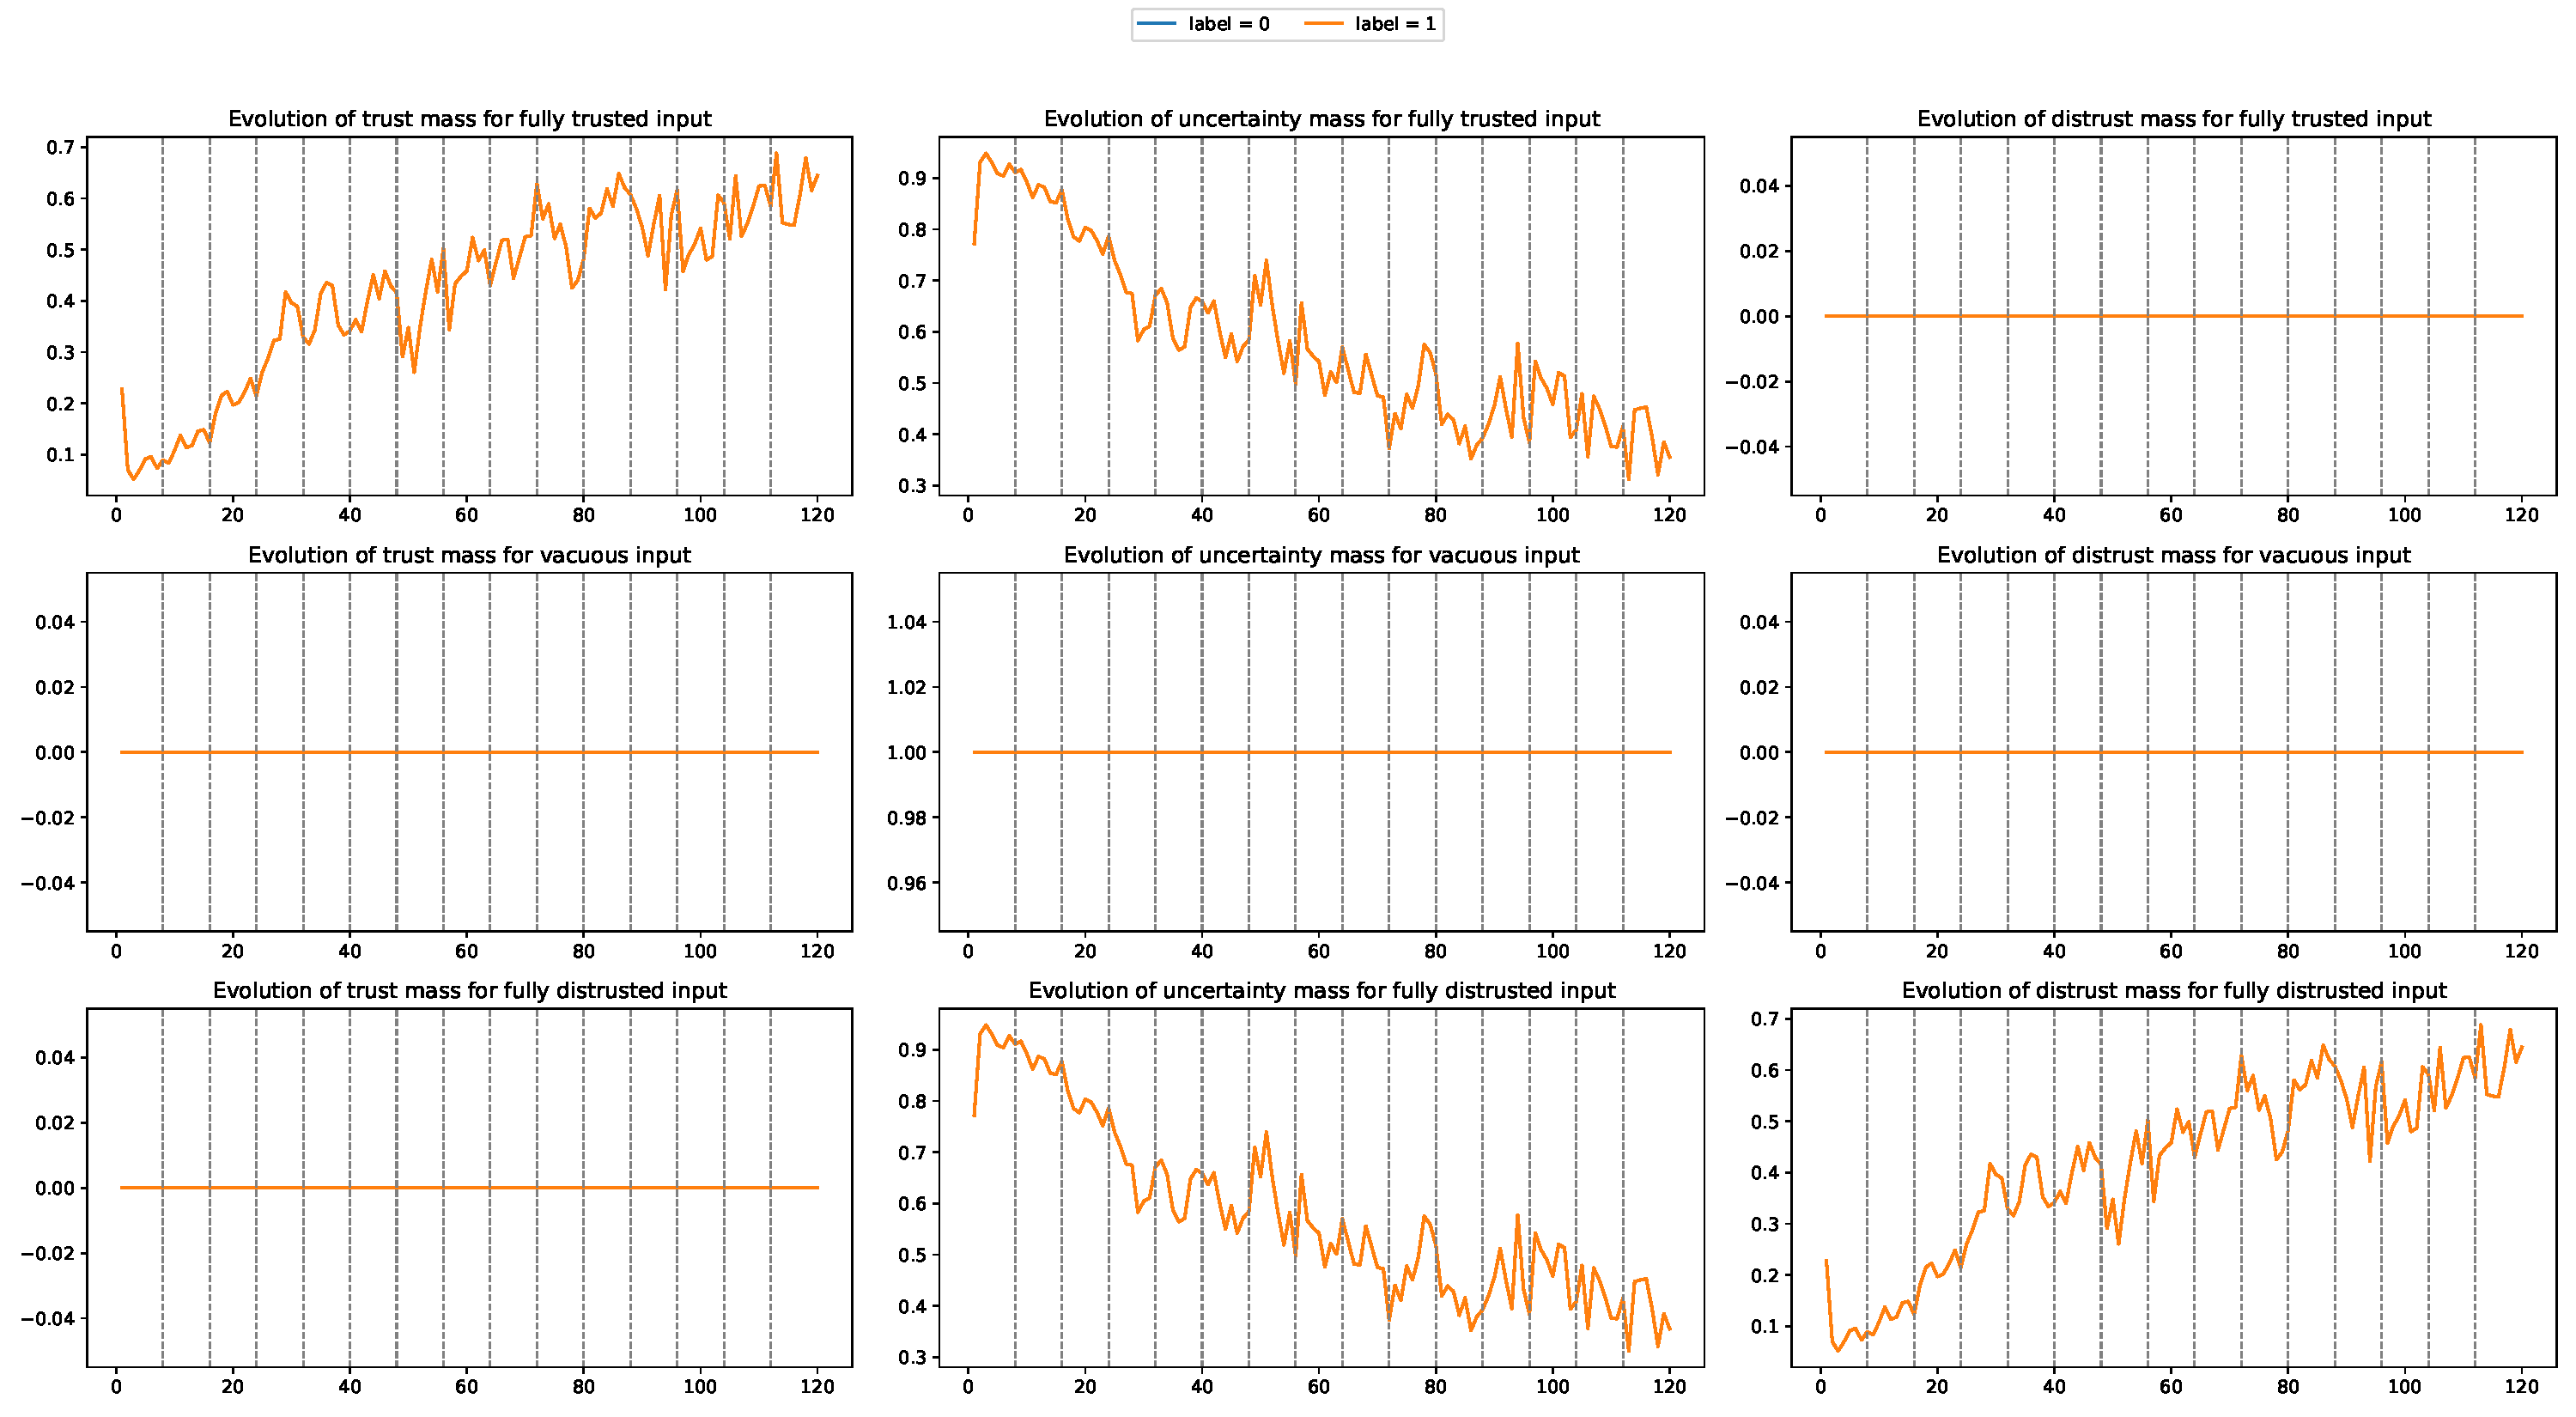
\includegraphics[width=\textwidth]{plots_v2/Cancer/eps=0.01/plot_ptas-t-t.pdf}
  \caption{Features trusted and labels trusted}
\end{figure}

\subsection{Cancer Model with \( \epsilon = 0.1 \)(\cref{exp:1})}\label{sec:rescancer0.1}
\begin{figure}[H]
  \includegraphics[width=\textwidth]{plots_v2/Cancer/eps=0.1/plot_ptas-d-d.pdf}
  \caption{Features distrusted and labels distrusted}
\end{figure}
\begin{figure}[H]
  \includegraphics[width=\textwidth]{plots_v2/Cancer/eps=0.1/plot_ptas-d-v.pdf}
  \caption{Features distrusted and labels vacuous}
\end{figure}
\begin{figure}[H]
  \includegraphics[width=\textwidth]{plots_v2/Cancer/eps=0.1/plot_ptas-d-t.pdf}
  \caption{Features distrusted and labels trusted}
\end{figure}
\begin{figure}[H]
  \includegraphics[width=\textwidth]{plots_v2/Cancer/eps=0.1/plot_ptas-v-d.pdf}
  \caption{Features vacuous and labels distrusted}
\end{figure}
\begin{figure}[H]
  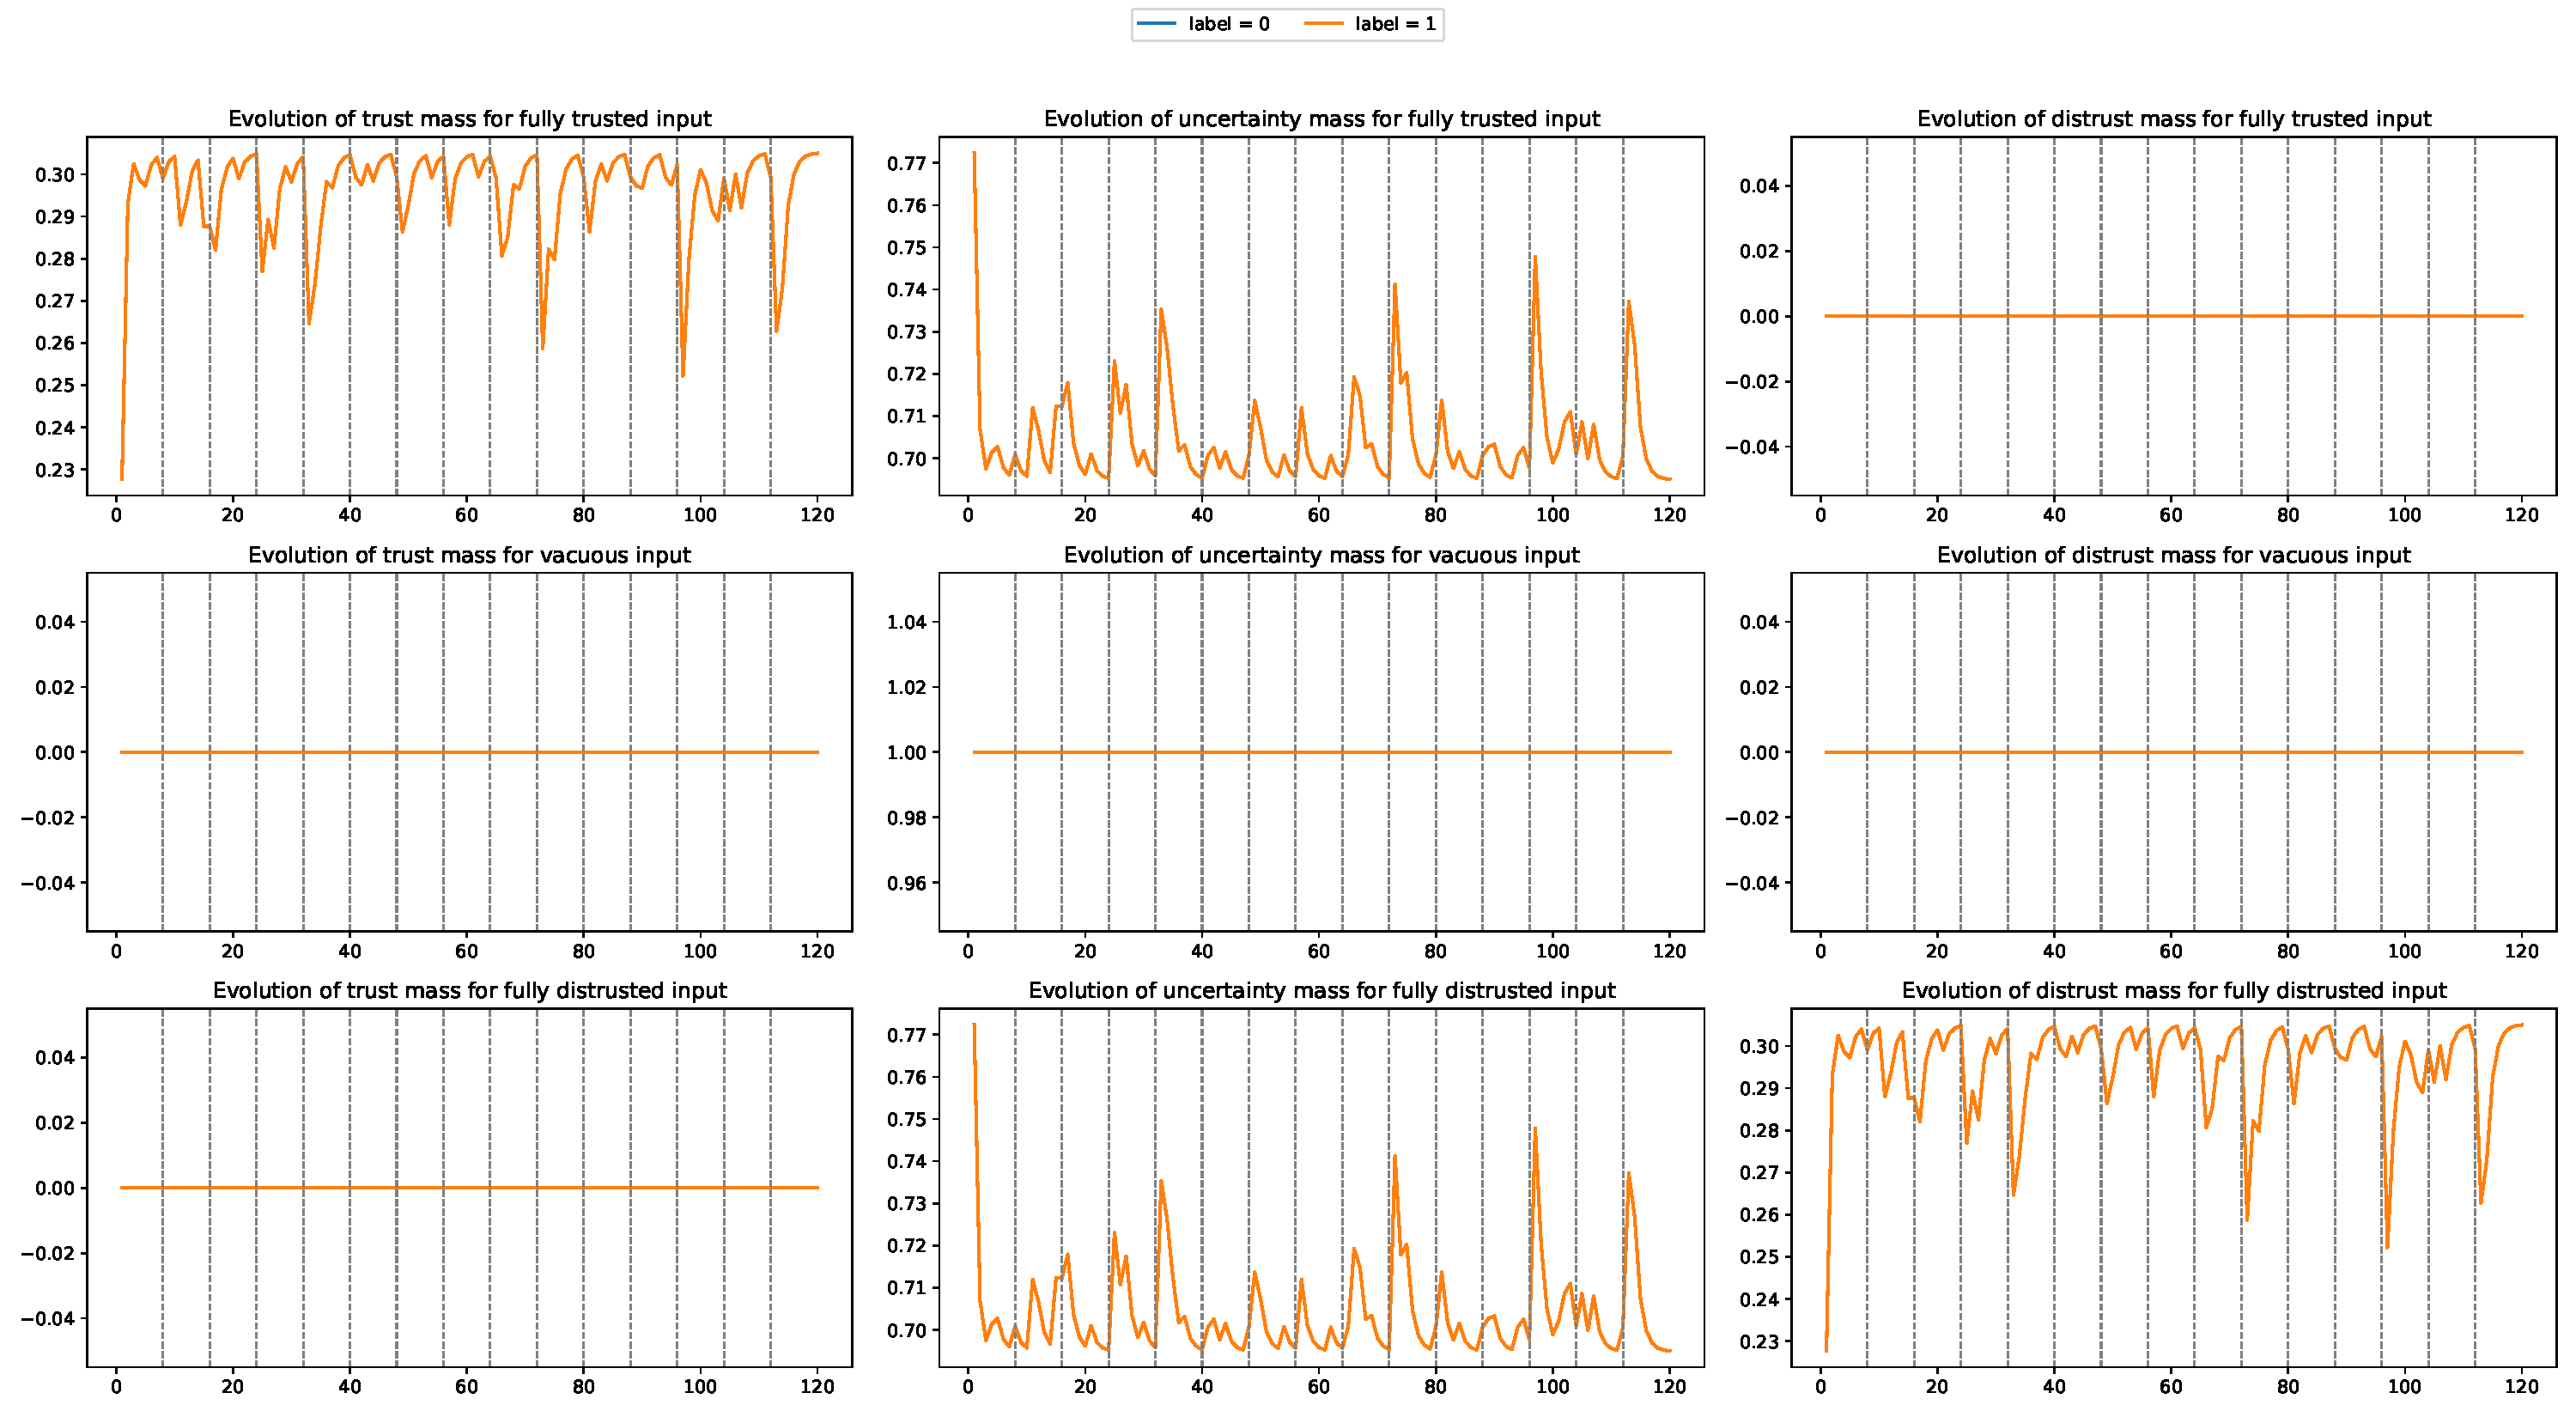
\includegraphics[width=\textwidth]{plots_v2/Cancer/eps=0.1/plot_ptas-v-v.pdf}
  \caption{Features vacuous and labels vacuous}
\end{figure}
\begin{figure}[H]
  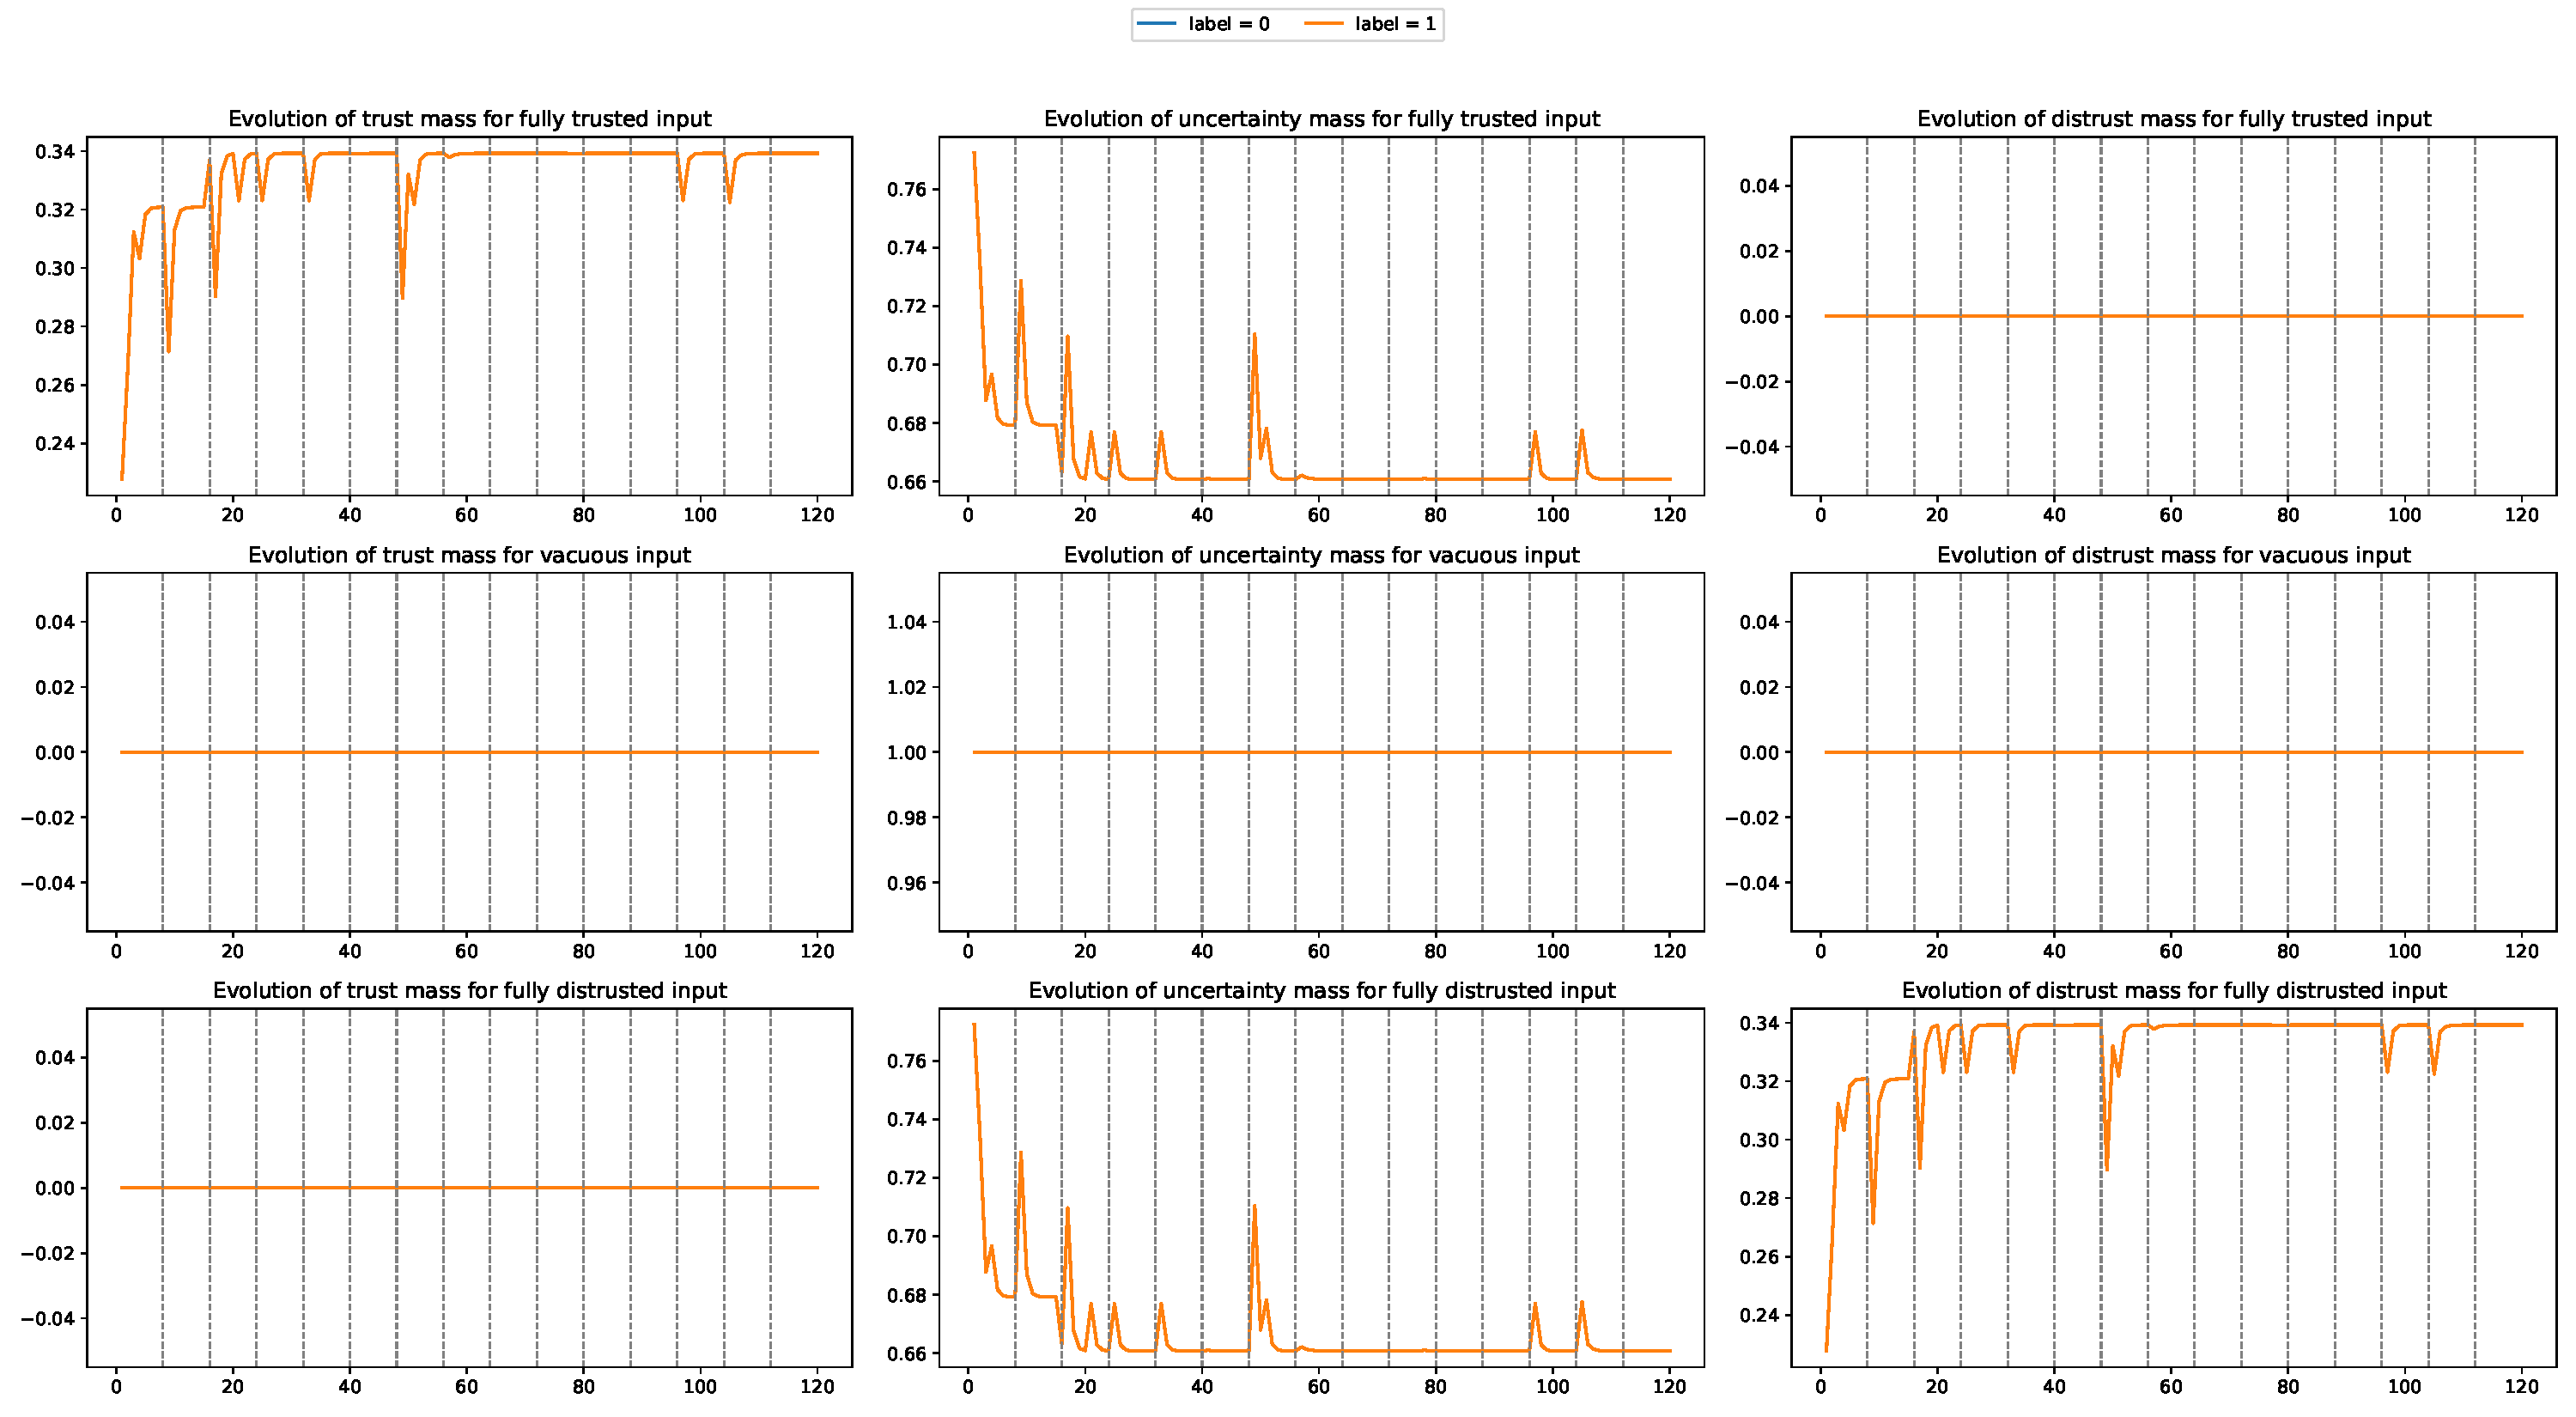
\includegraphics[width=\textwidth]{plots_v2/Cancer/eps=0.1/plot_ptas-v-t.pdf}
  \caption{Features vacuous and labels trusted}
\end{figure}
\begin{figure}[H]
  \includegraphics[width=\textwidth]{plots_v2/Cancer/eps=0.1/plot_ptas-t-d.pdf}
  \caption{Features trusted and labels distrusted}
\end{figure}
\begin{figure}[H]
  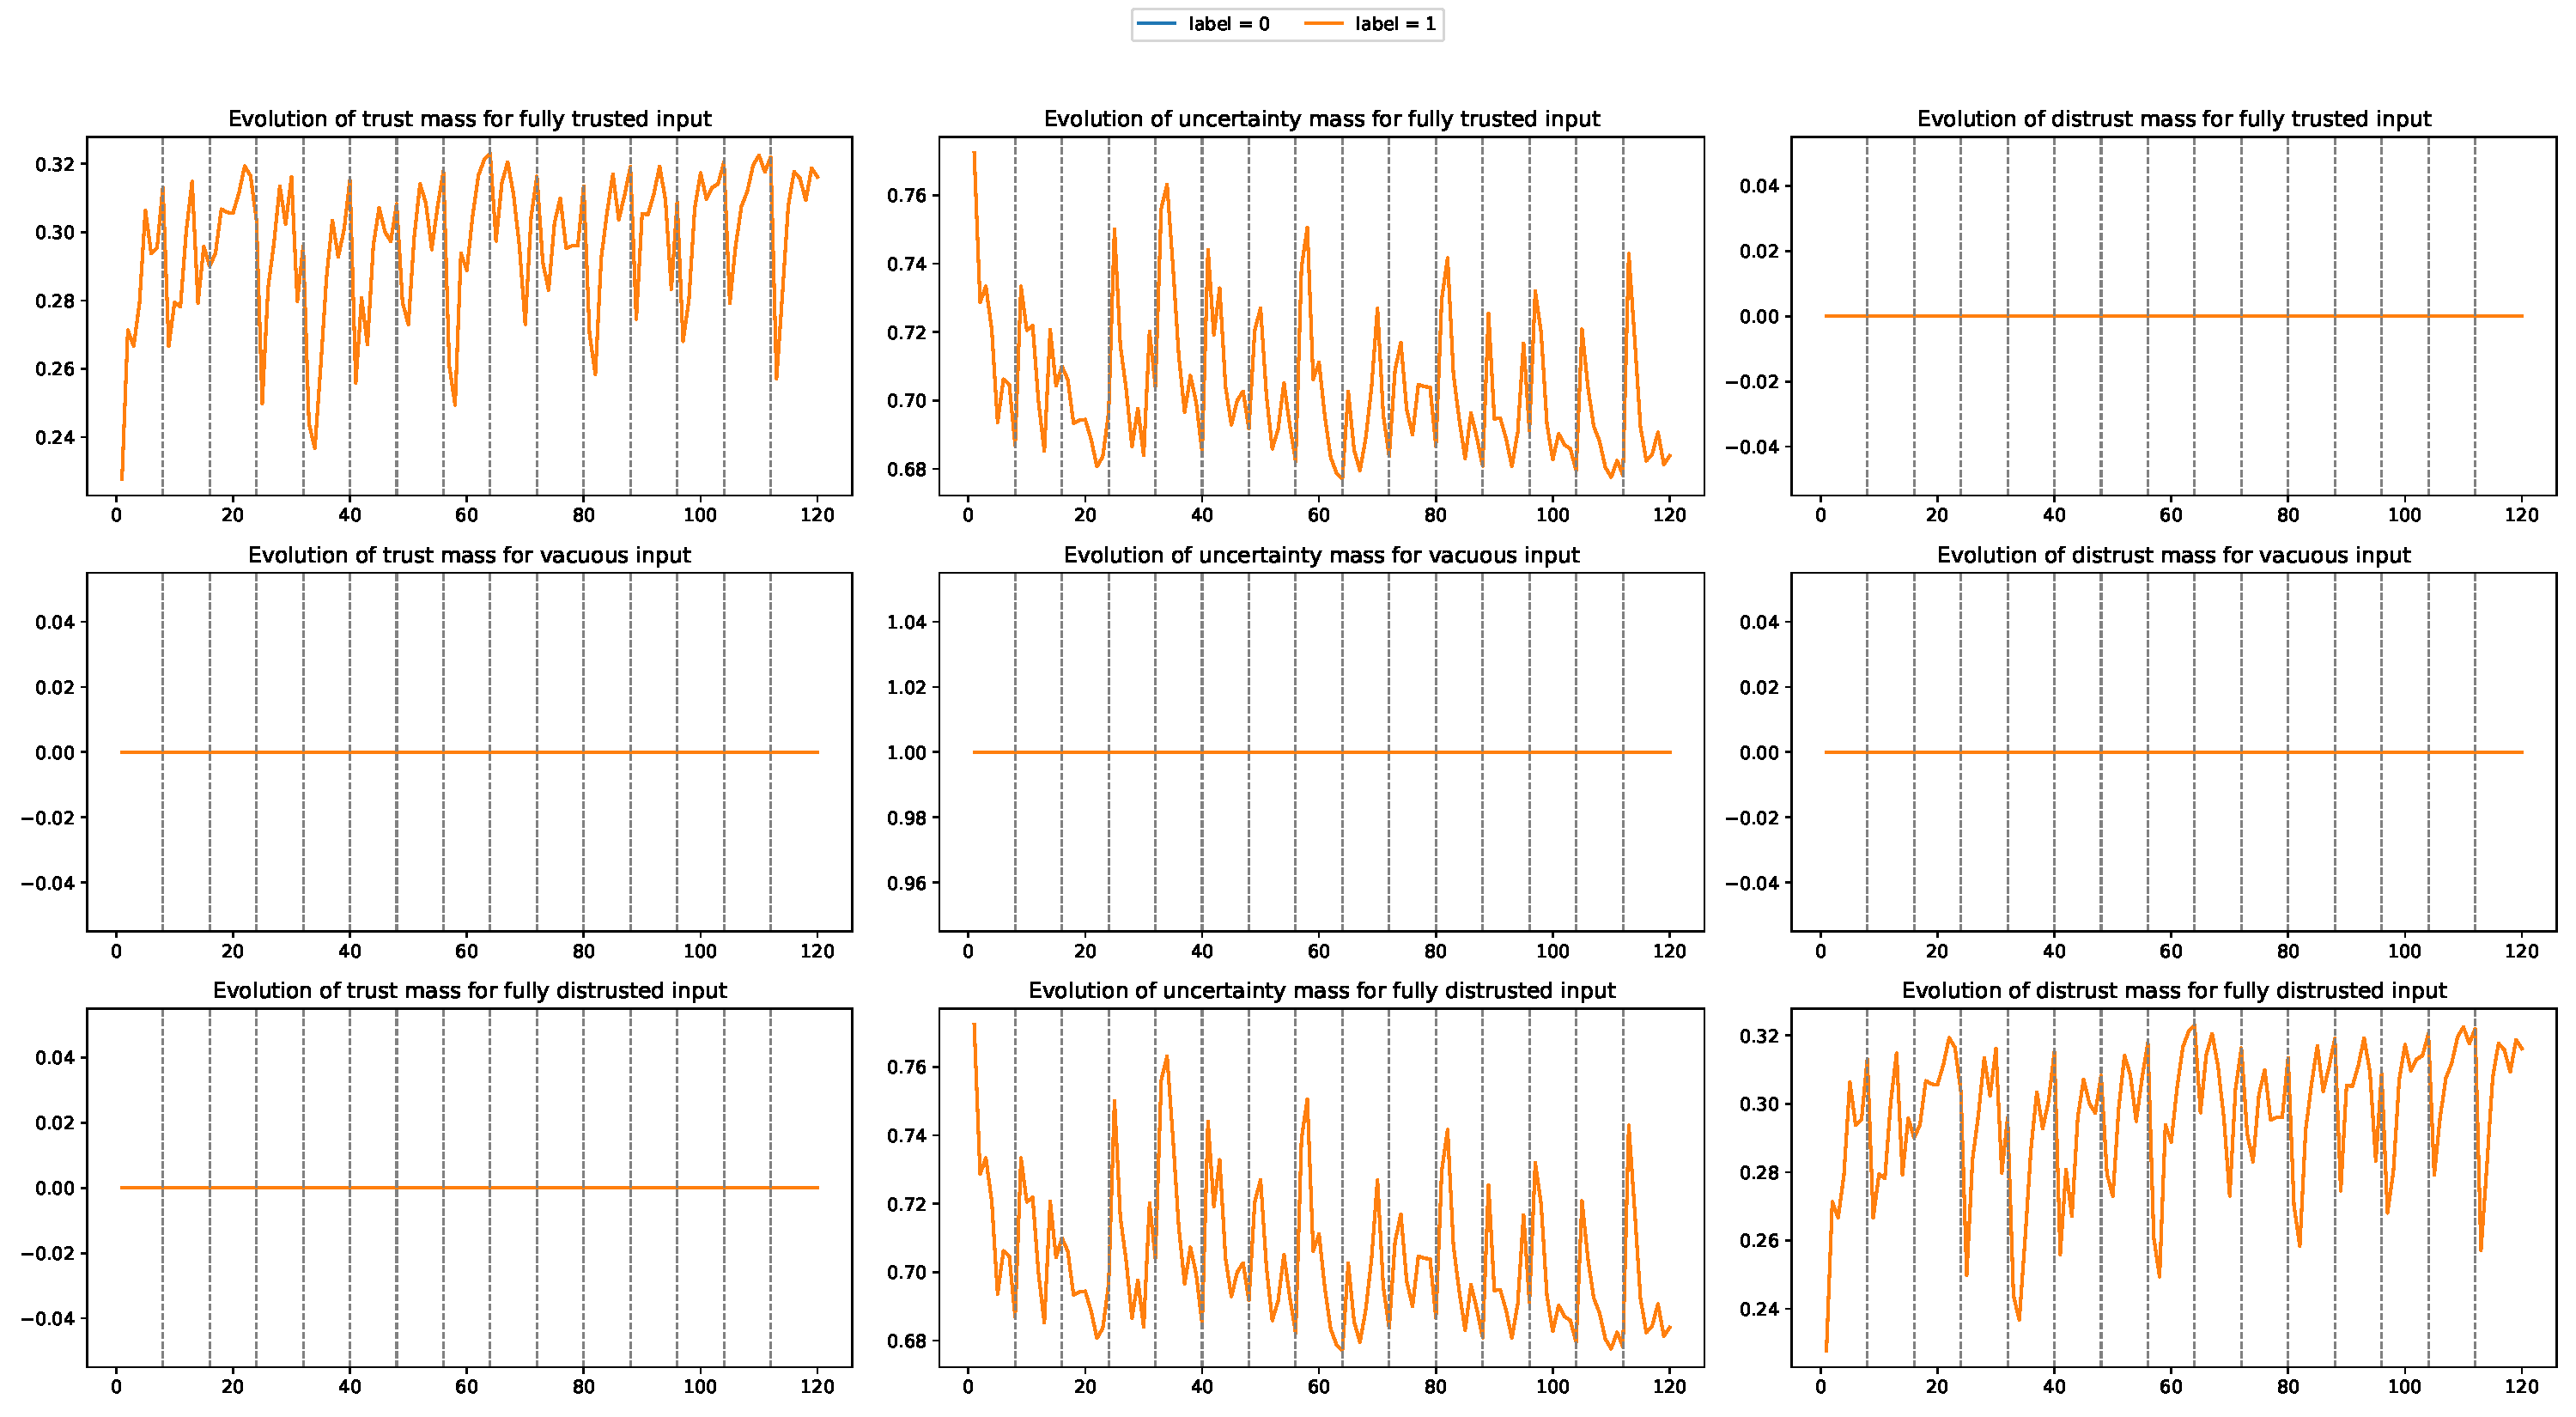
\includegraphics[width=\textwidth]{plots_v2/Cancer/eps=0.1/plot_ptas-t-v.pdf}
  \caption{Features trusted and labels vacuous}
\end{figure}
\begin{figure}[H]
  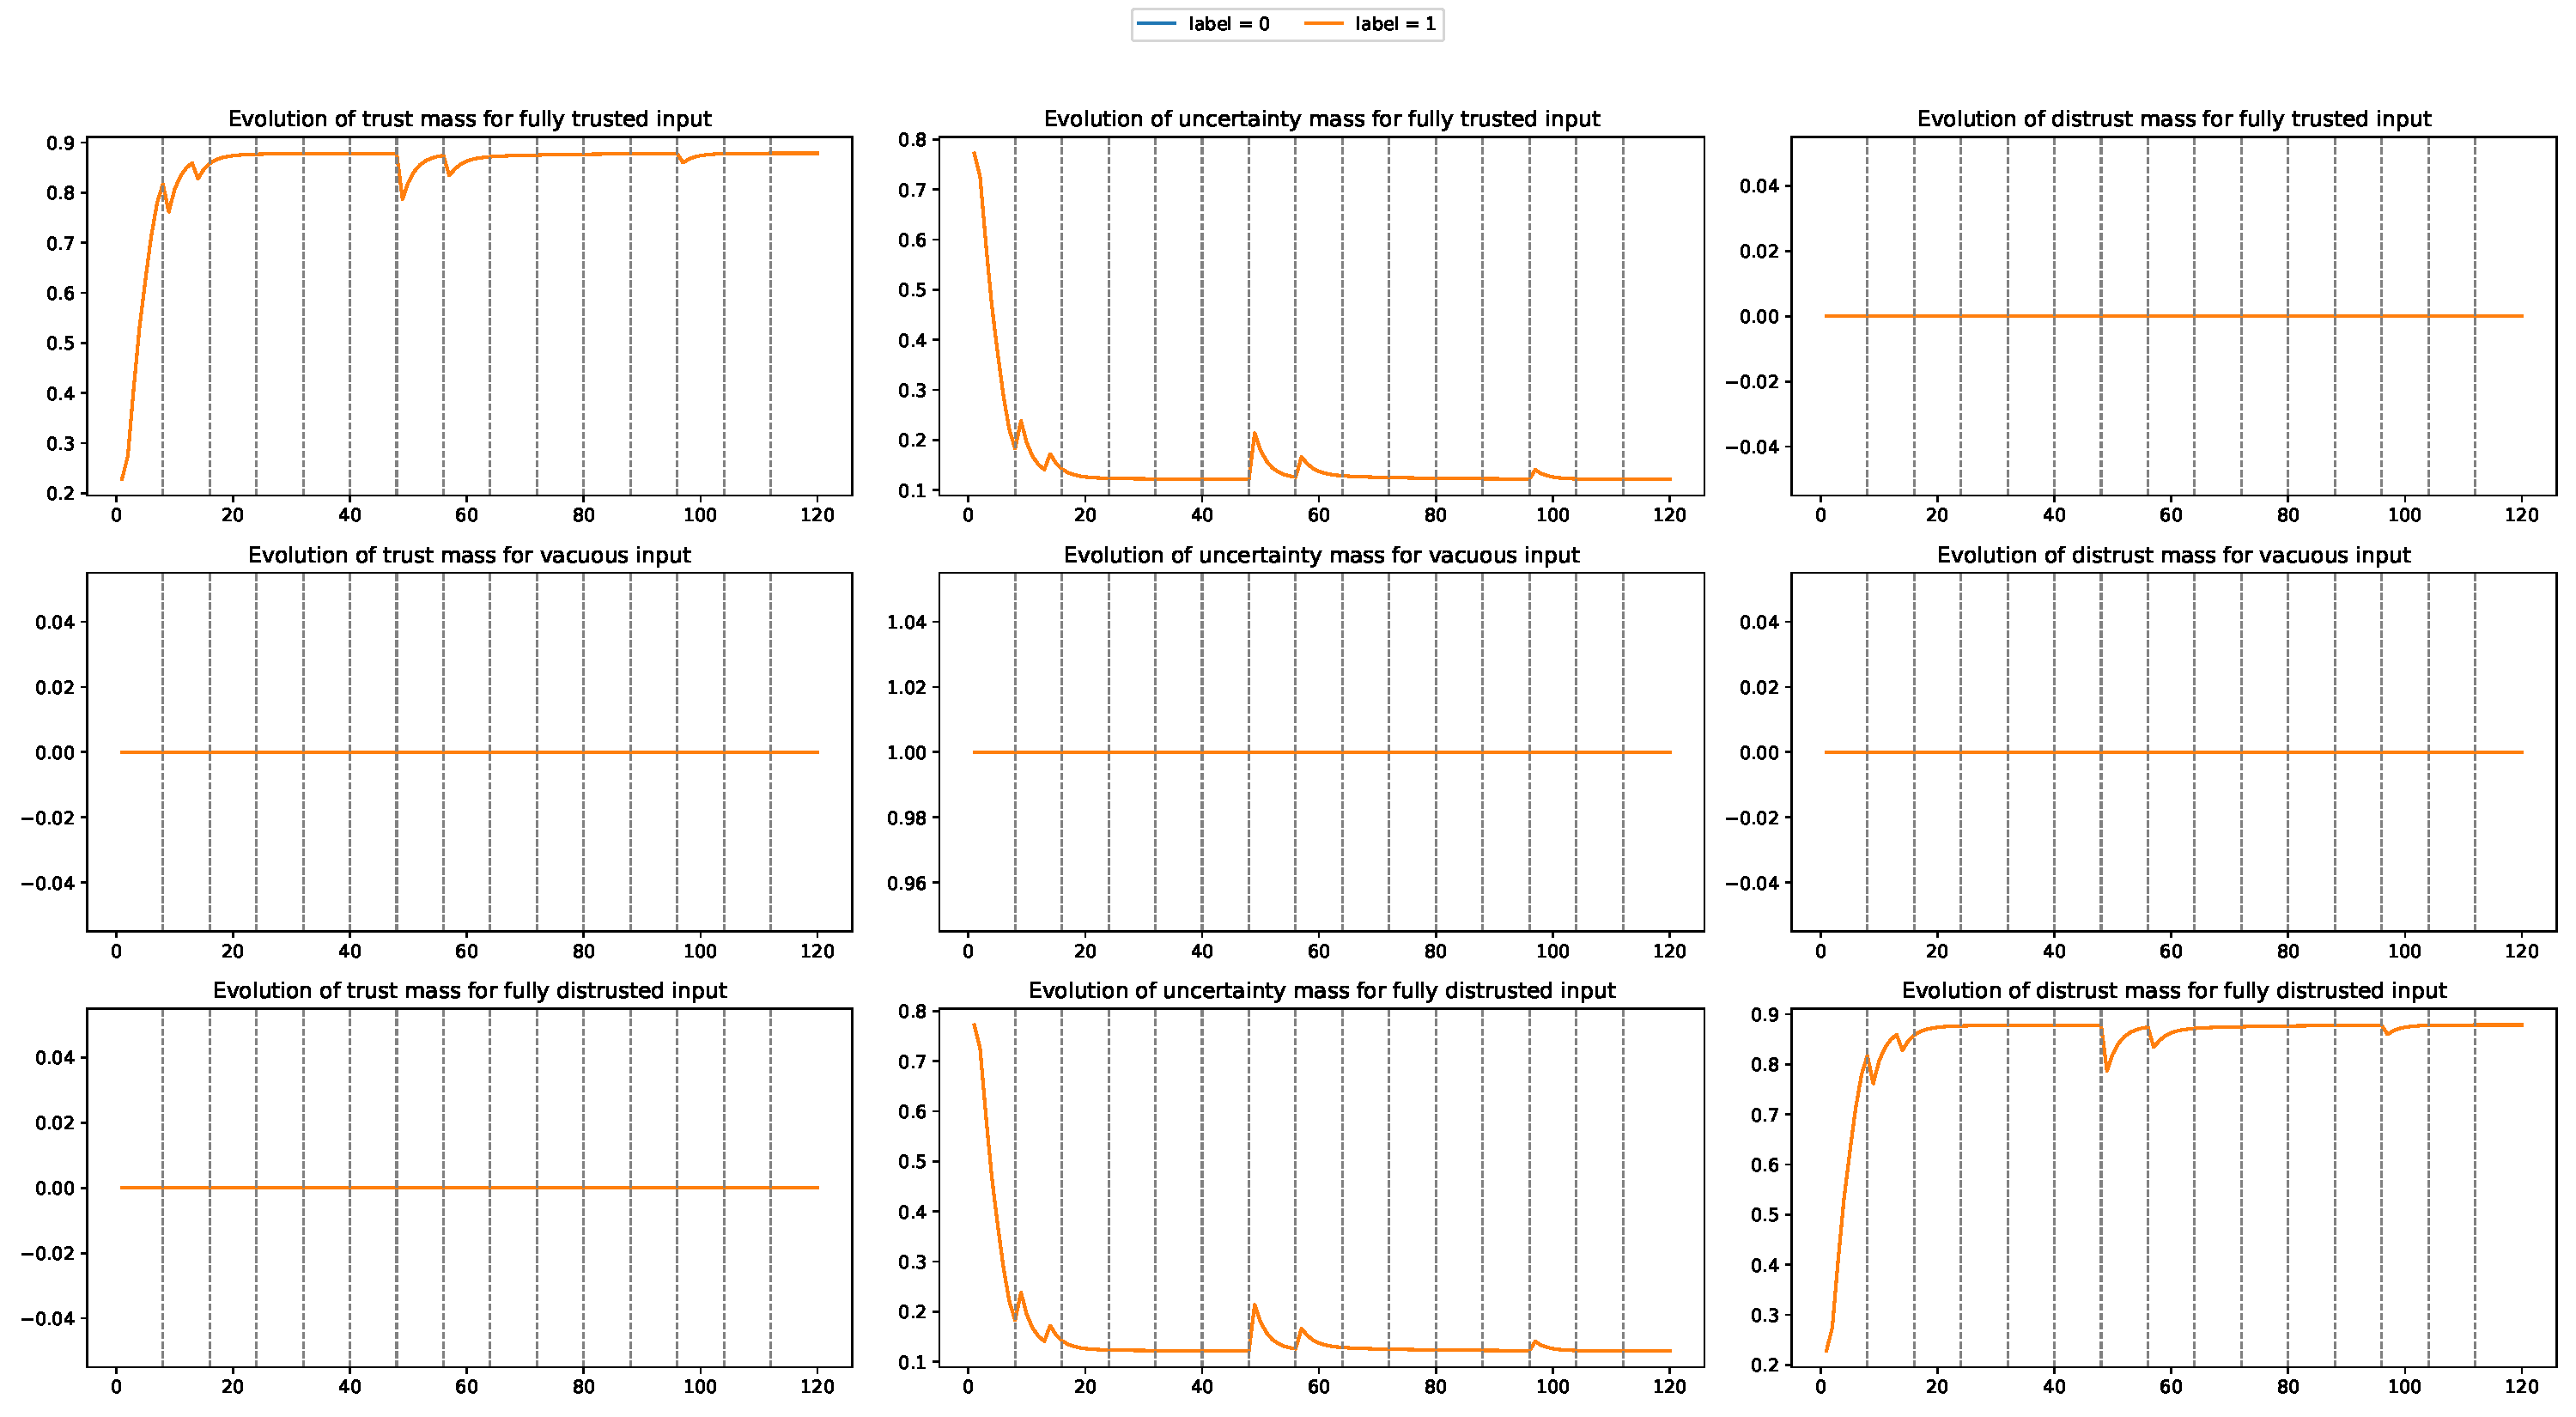
\includegraphics[width=\textwidth]{plots_v2/Cancer/eps=0.1/plot_ptas-t-t.pdf}
  \caption{Features trusted and labels trusted}
\end{figure}

\subsection{Accuracy Evolution for the Cancer Model (\cref{exp:1})}\label{sec:resmnistaccapp}
\begin{figure}[H]
\centering
\begin{subfigure}[b]{0.32\textwidth}
  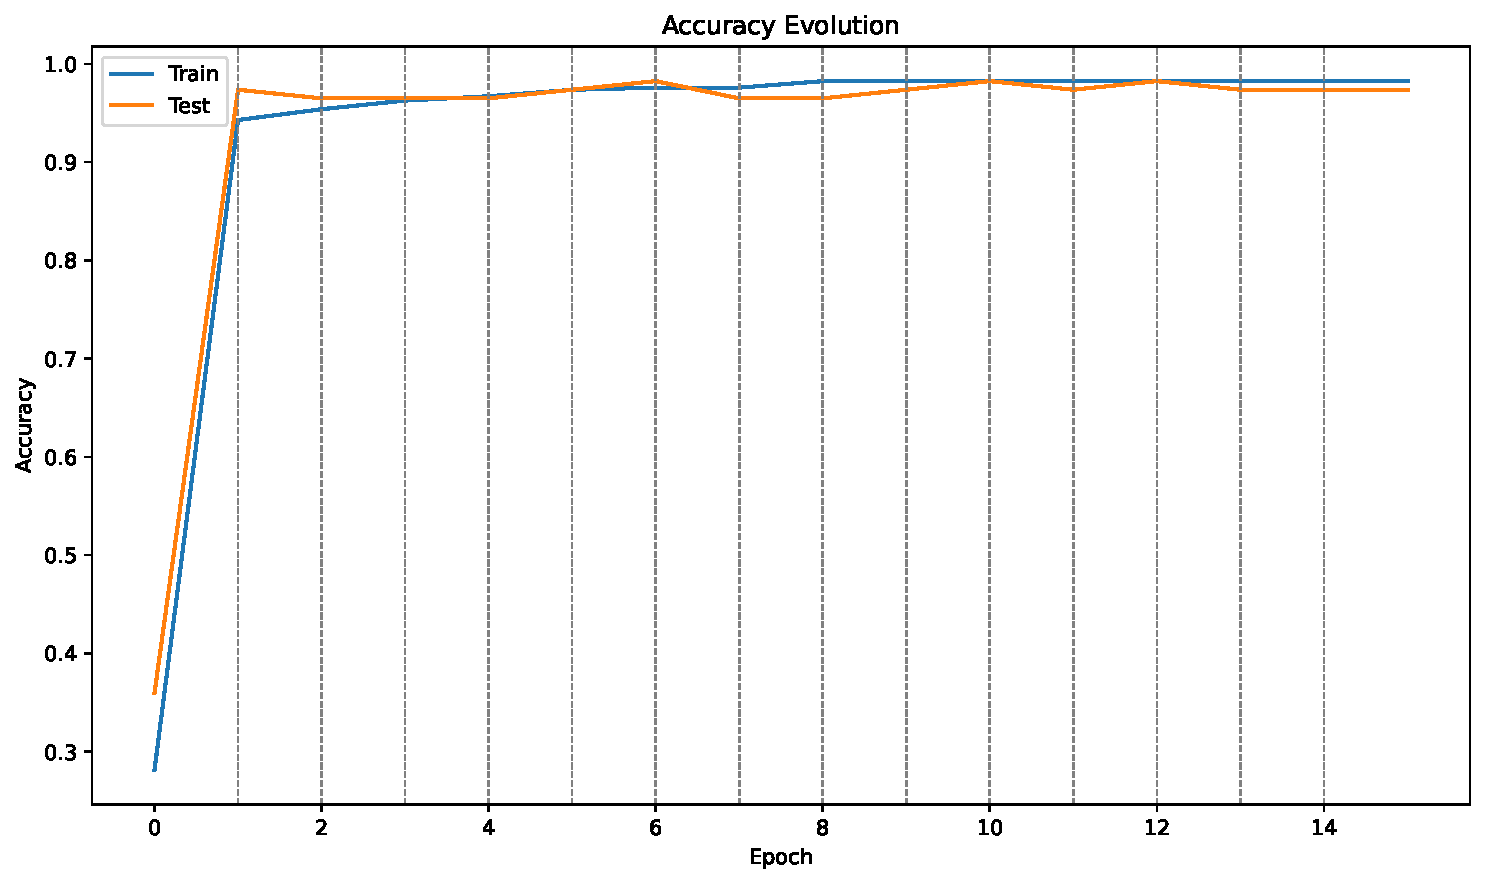
\includegraphics[width=\textwidth]{plots_v2/Cancer/eps=0.1/accuracy_evolution-t-t.pdf}
  \caption{Clean Features and Labels}
\end{subfigure}
\begin{subfigure}[b]{0.32\textwidth}
  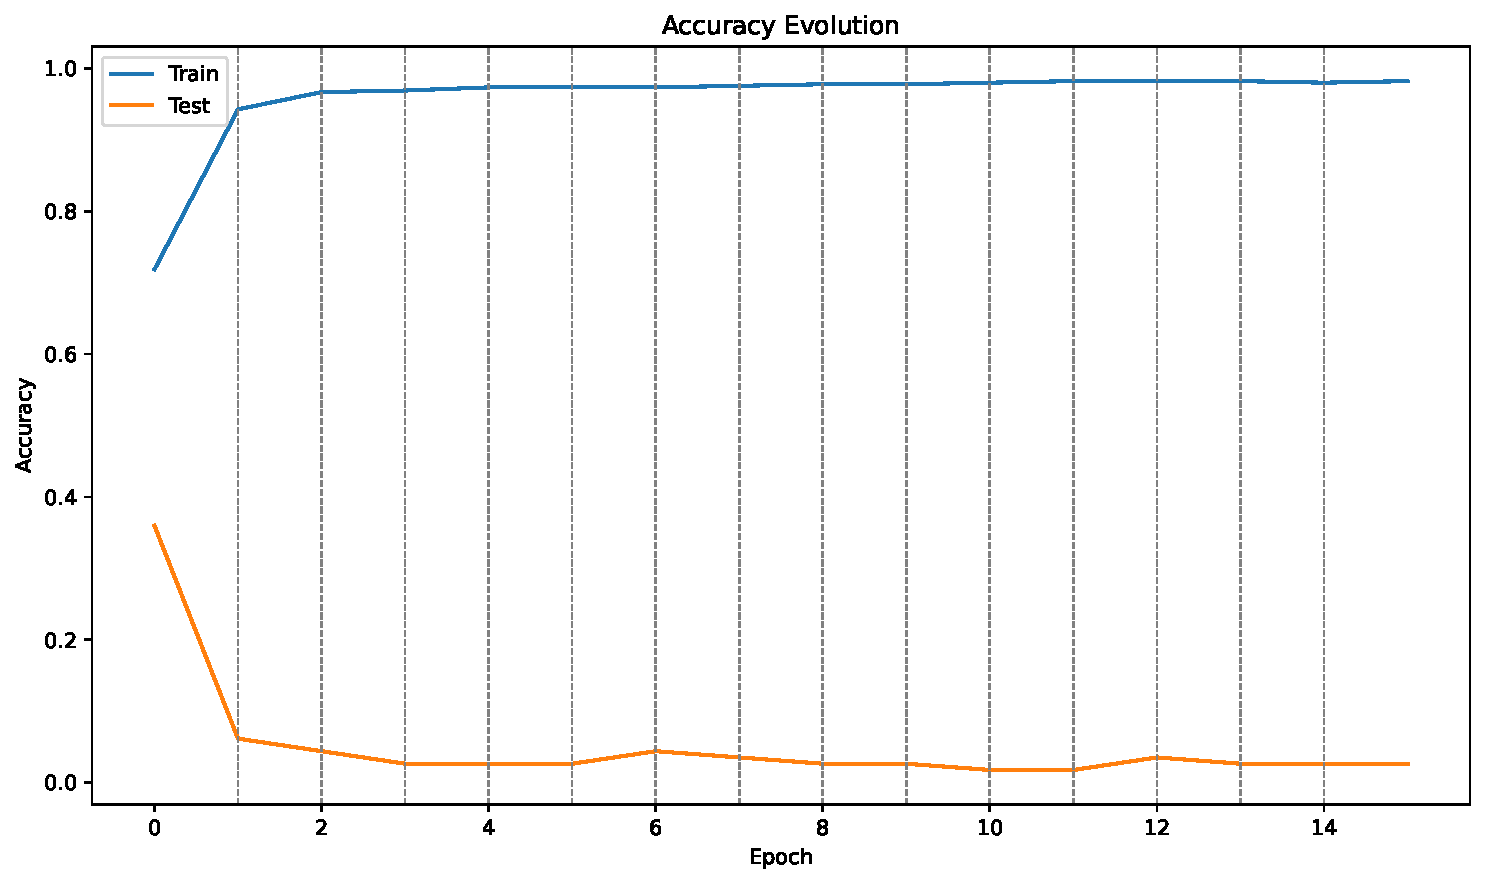
\includegraphics[width=\textwidth]{plots_v2/Cancer/eps=0.1/accuracy_evolution-t-d.pdf}
  \caption{Clean Features and Corrupted Labels}
\end{subfigure}
\begin{subfigure}[b]{0.32\textwidth}
  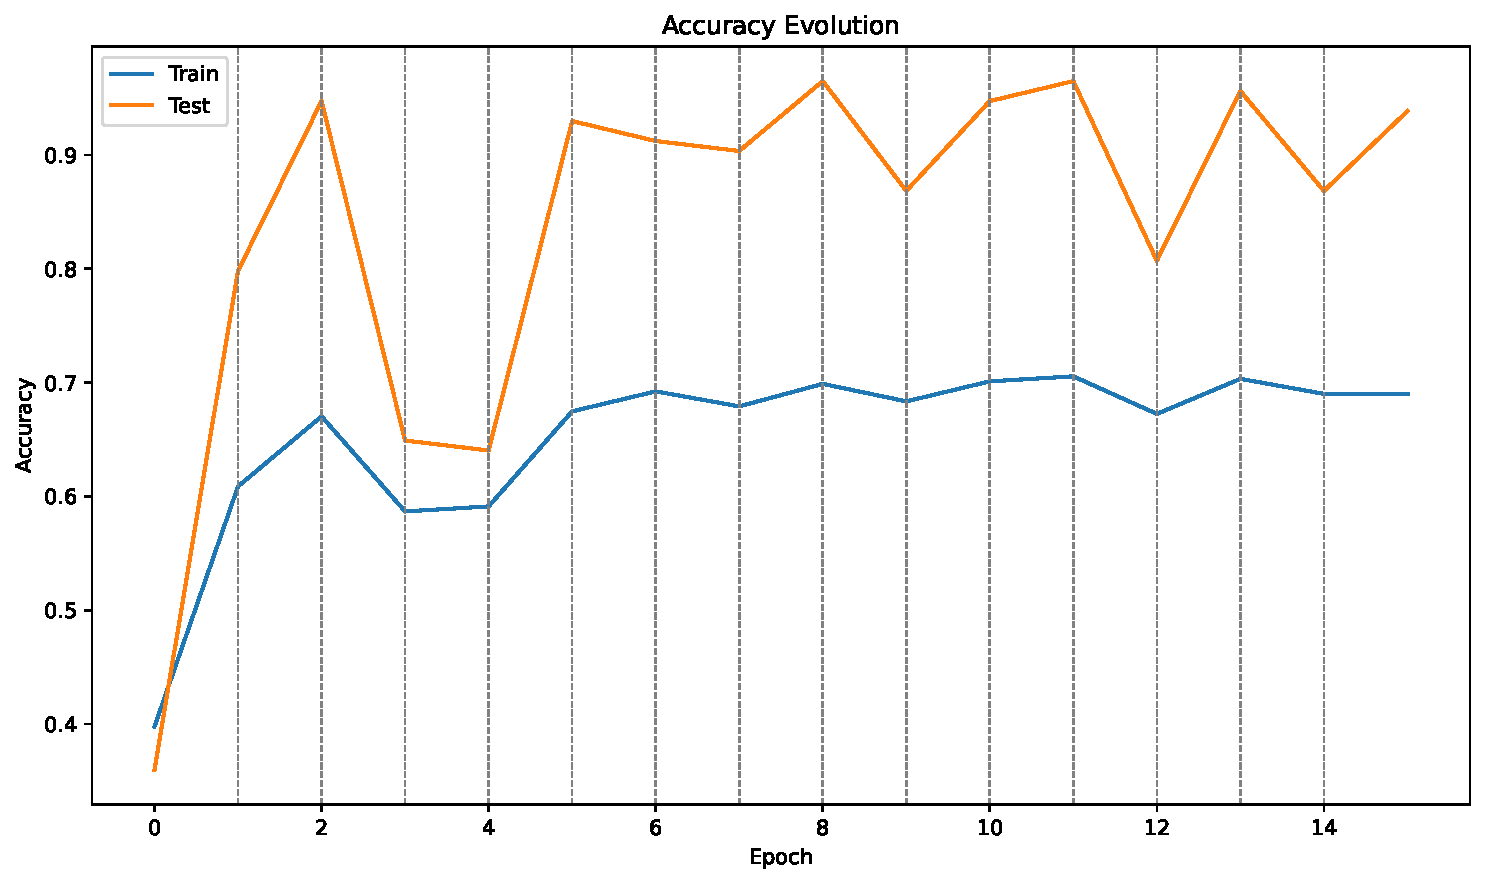
\includegraphics[width=\textwidth]{plots_v2/Cancer/eps=0.1/accuracy_evolution-t-v.pdf}
  \caption{Clean Features and Noisy Labels}
\end{subfigure}
\begin{subfigure}[b]{0.32\textwidth}
  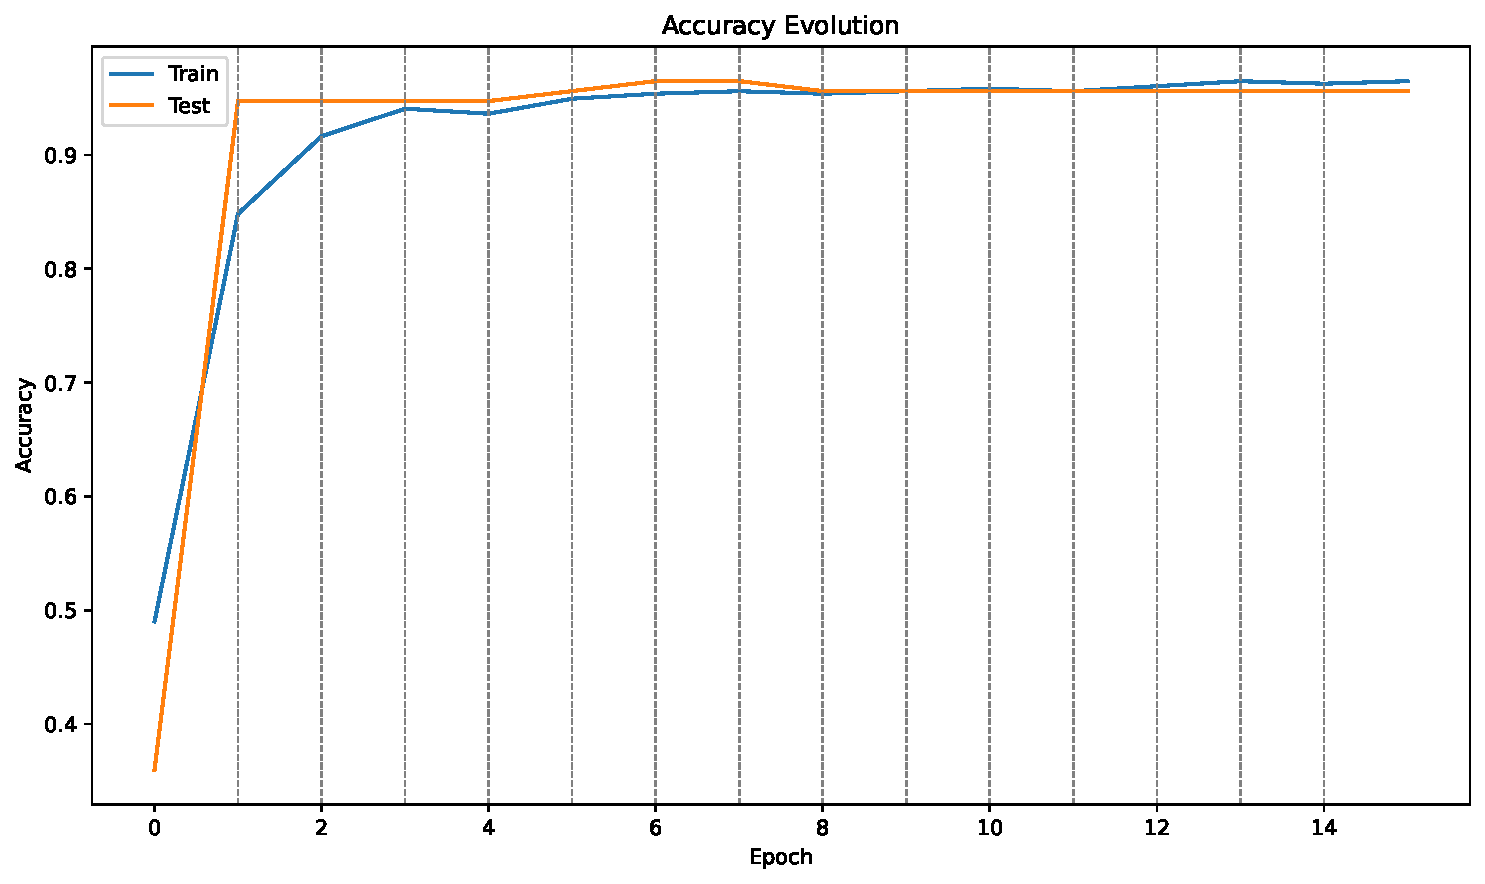
\includegraphics[width=\textwidth]{plots_v2/Cancer/eps=0.1/accuracy_evolution-v-t.pdf}
  \caption{Noisy Features and Clean Labels}
\end{subfigure}
\begin{subfigure}[b]{0.32\textwidth}
  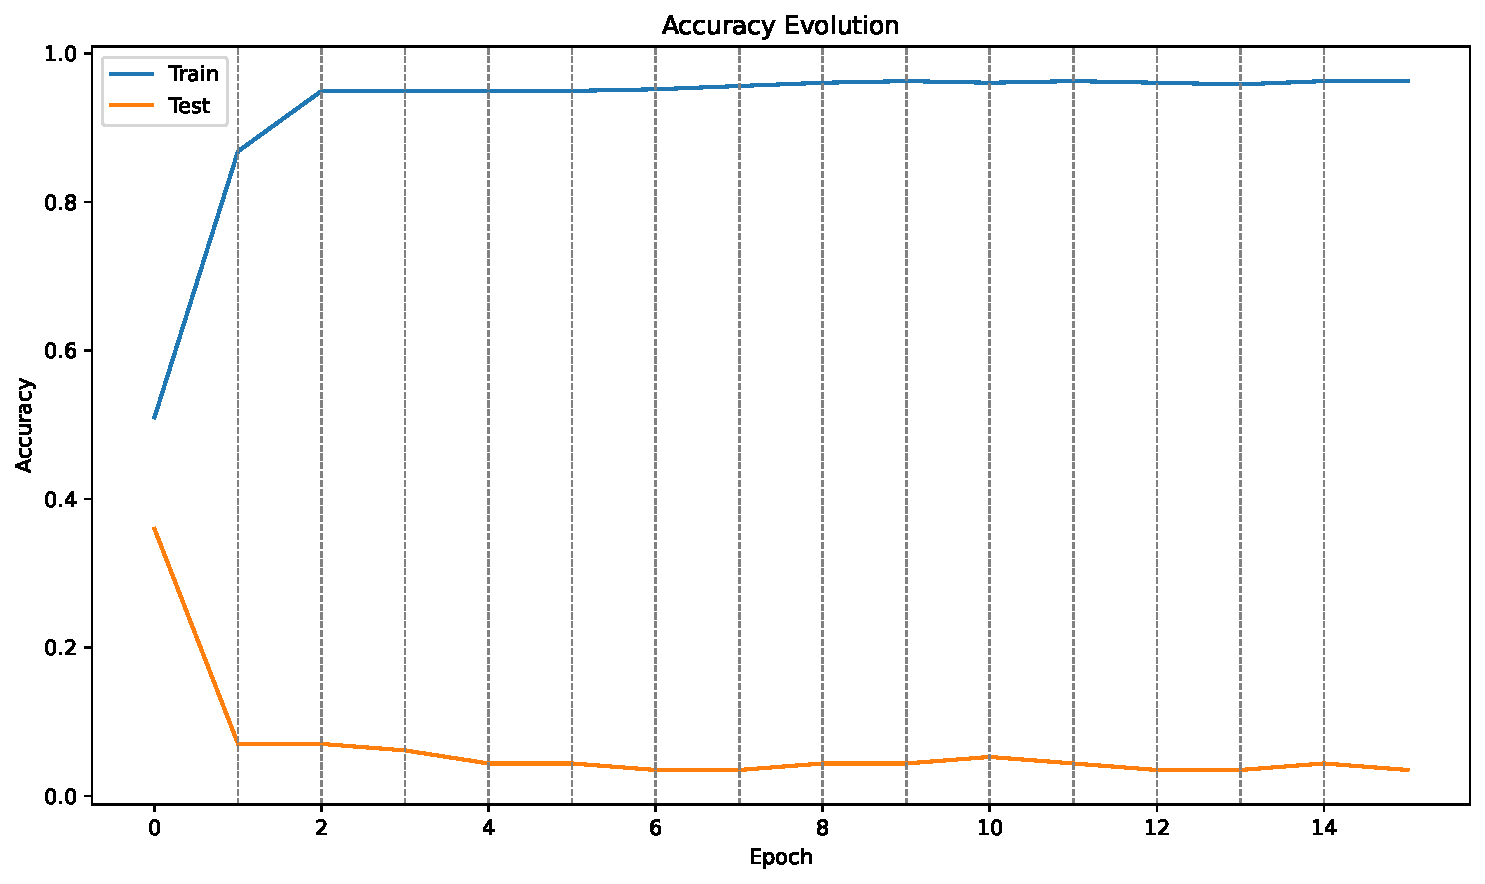
\includegraphics[width=\textwidth]{plots_v2/Cancer/eps=0.1/accuracy_evolution-v-d.pdf}
  \caption{Noisy Features and Corrupted Labels}
\end{subfigure}
\begin{subfigure}[b]{0.32\textwidth}
  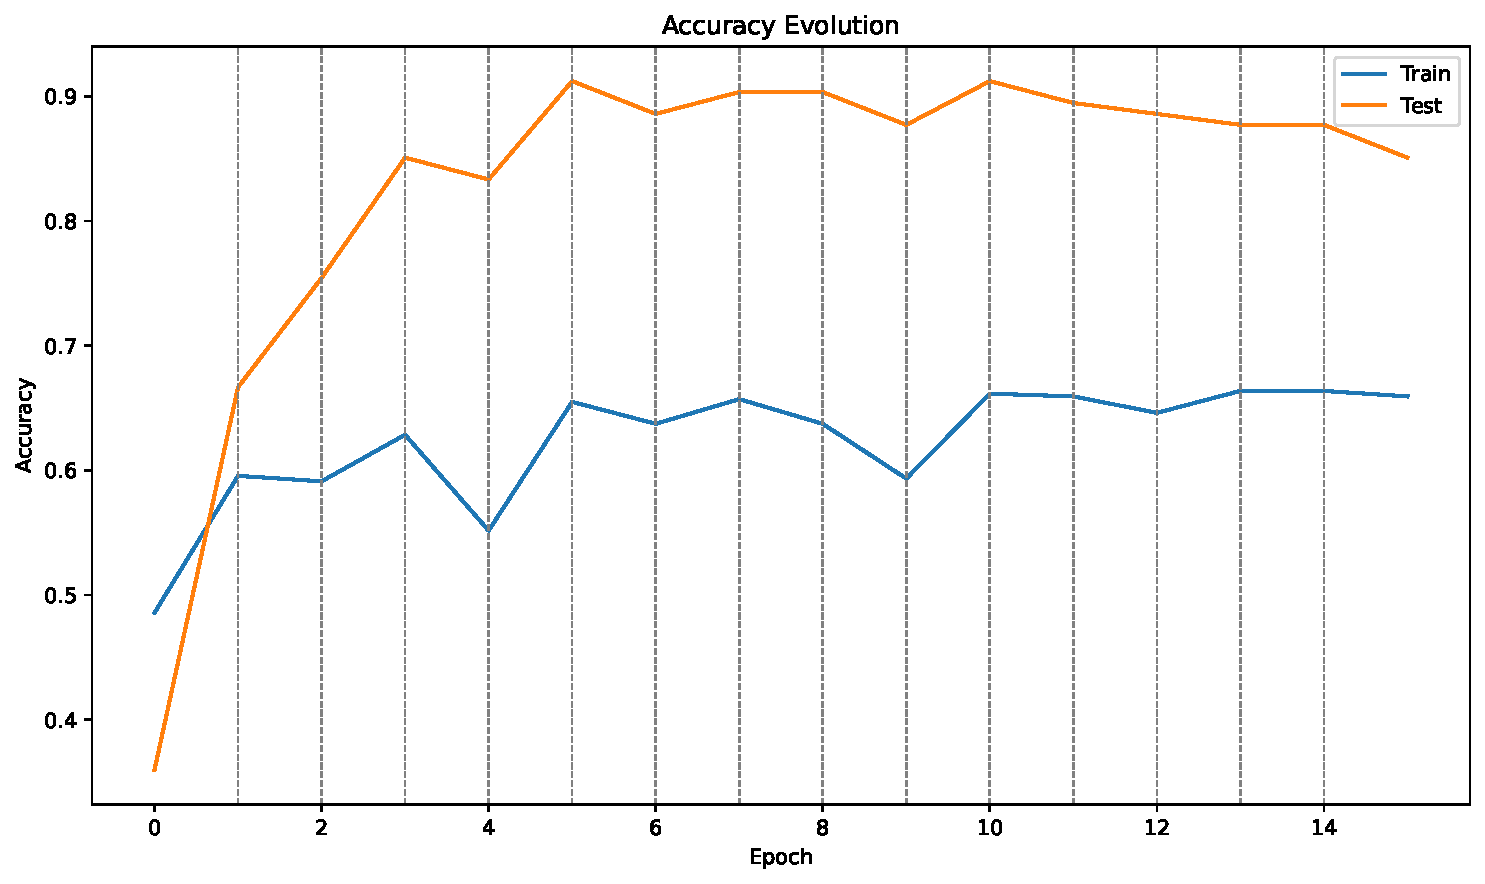
\includegraphics[width=\textwidth]{plots_v2/Cancer/eps=0.1/accuracy_evolution-v-v.pdf}
  \caption{Noisy Features and Noisy Labels}
\end{subfigure}
\begin{subfigure}[b]{0.32\textwidth}
  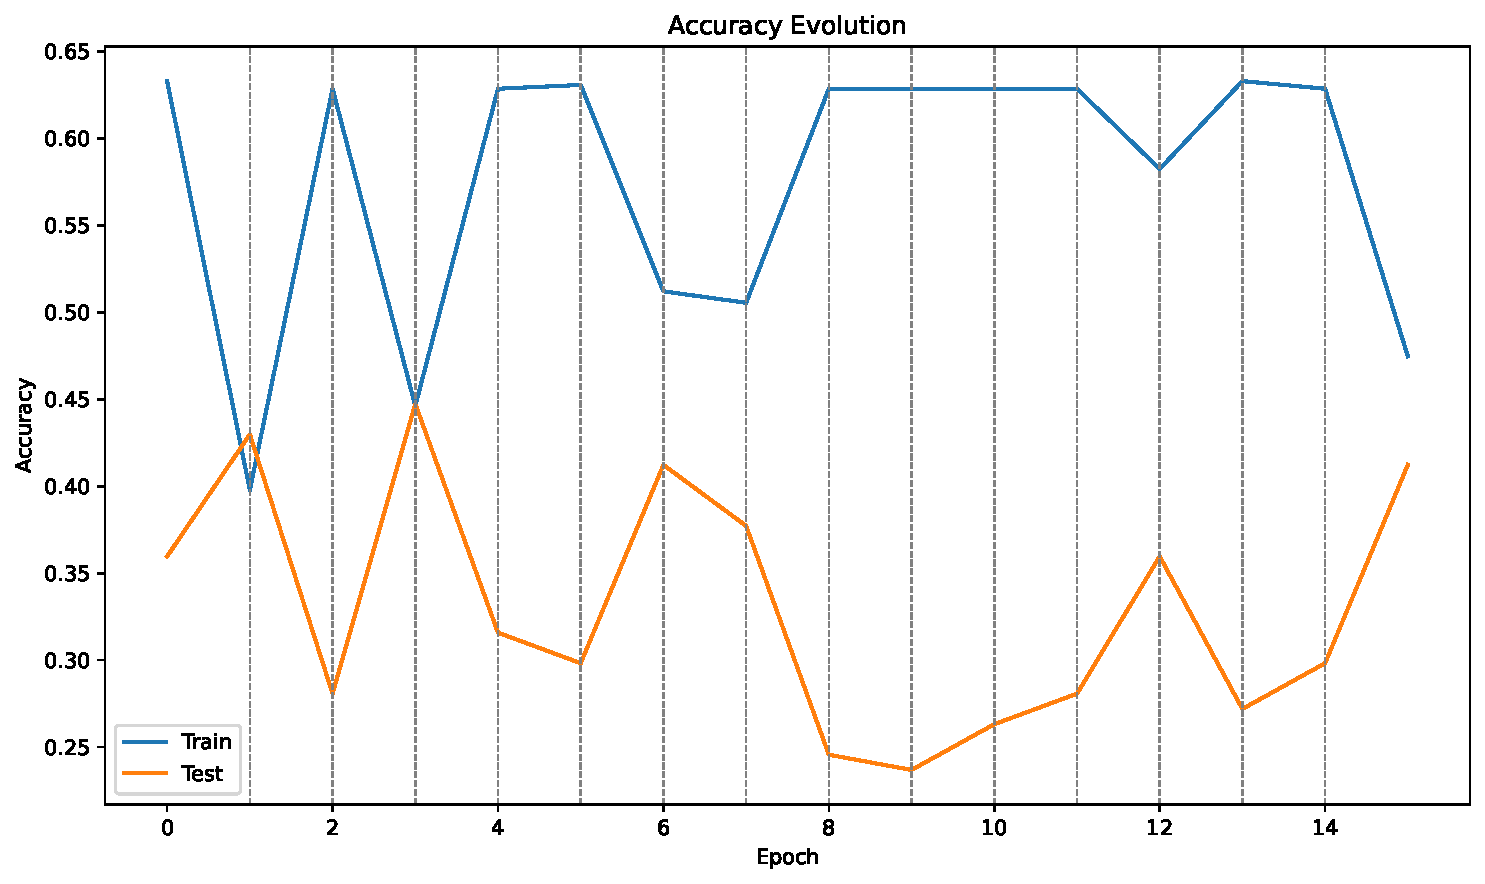
\includegraphics[width=\textwidth]{plots_v2/Cancer/eps=0.1/accuracy_evolution-d-t.pdf}
  \caption{Corrupted Features and Clean Labels}
\end{subfigure}
\begin{subfigure}[b]{0.32\textwidth}
  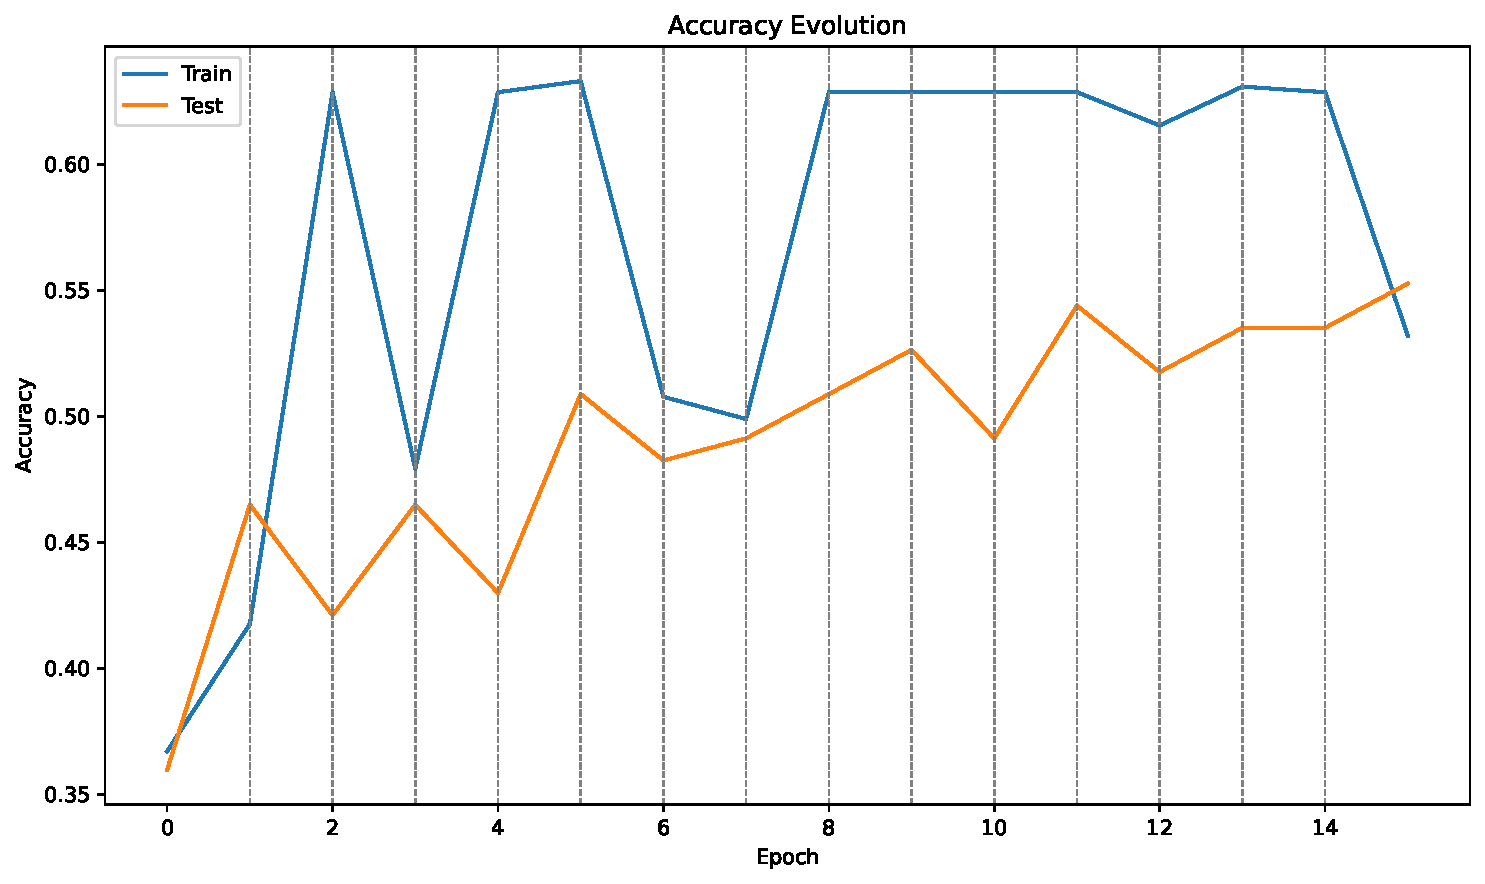
\includegraphics[width=\textwidth]{plots_v2/Cancer/eps=0.1/accuracy_evolution-d-d.pdf}
  \caption{Corrupted Features and Corrupted Labels}
\end{subfigure}
\begin{subfigure}[b]{0.32\textwidth}
  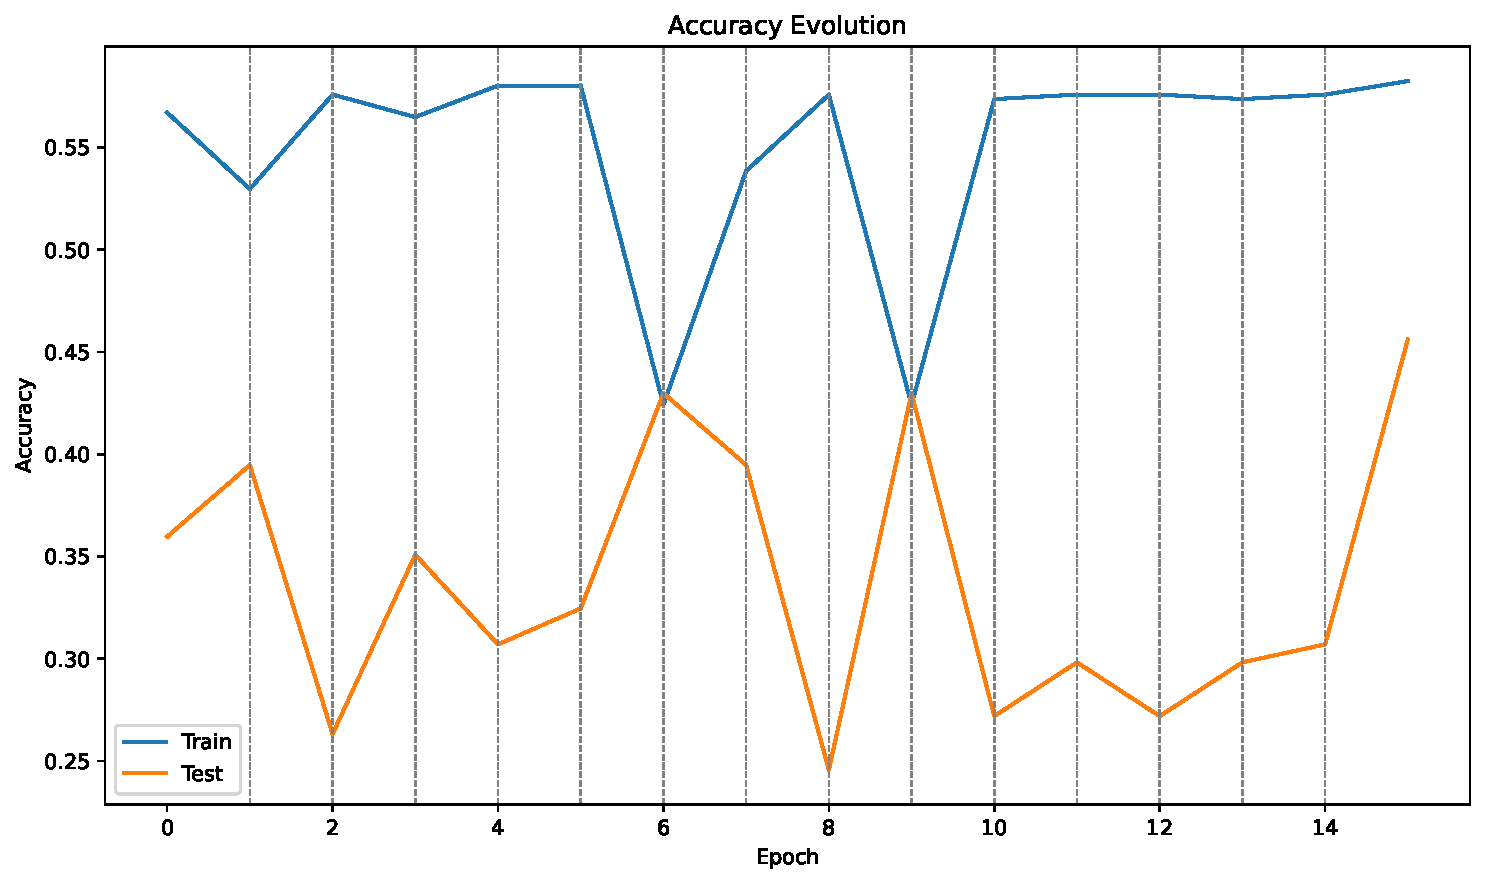
\includegraphics[width=\textwidth]{plots_v2/Cancer/eps=0.1/accuracy_evolution-d-v.pdf}
  \caption{Corrupted Features and Noisy Labels}
\end{subfigure}
\caption{Accuracy evolution of the Cancer model under different combinations of clean, corrupted, and noisy features and labels.}
\label{fig:Acccancer}
\end{figure}
% \begin{figure}[H]
%     \centering
%     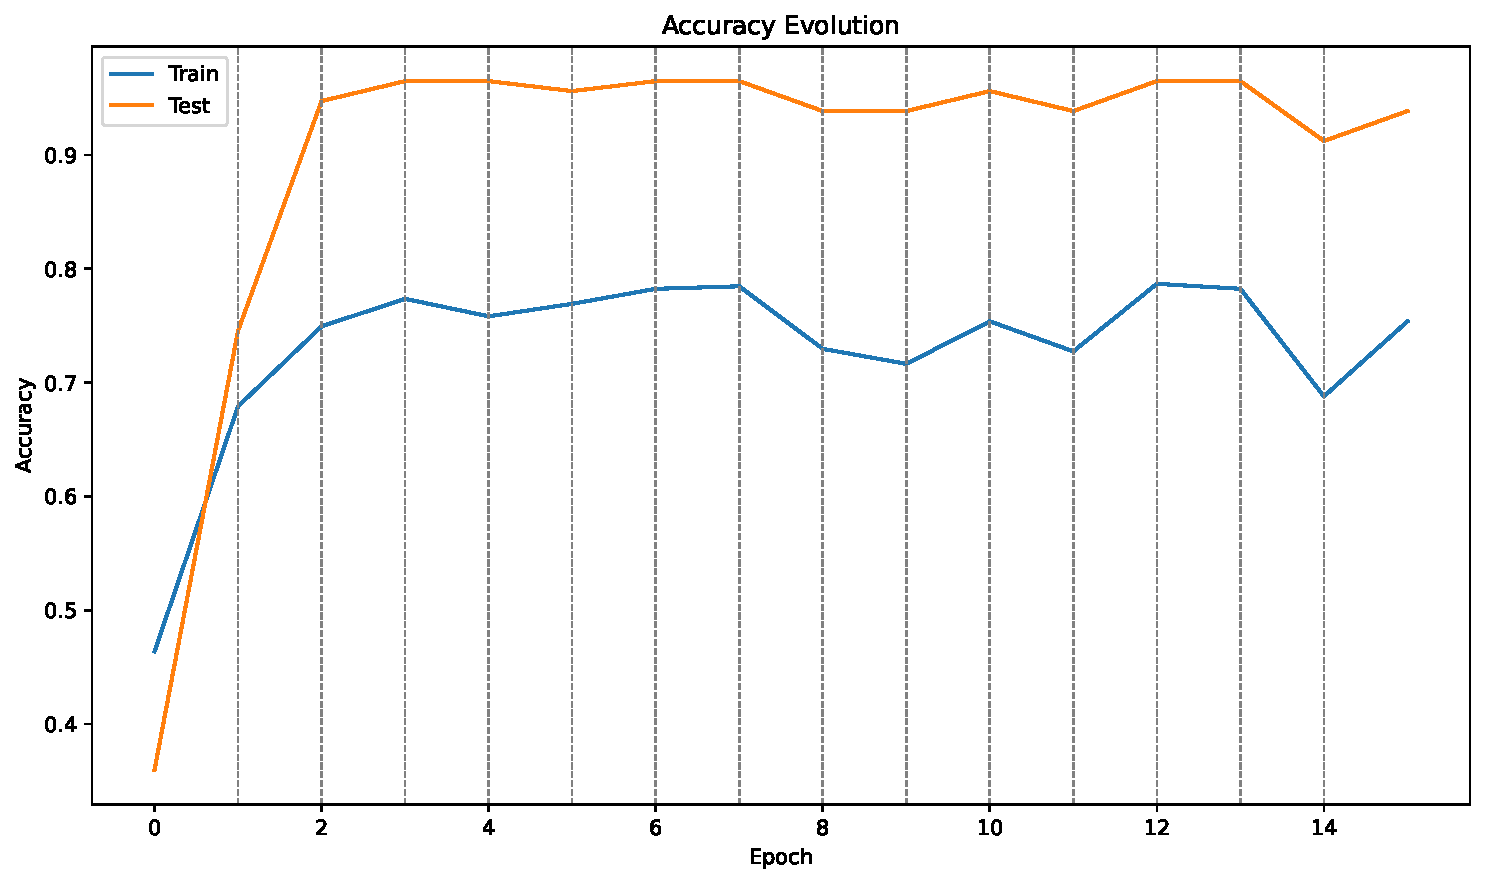
\includegraphics[width=0.8\linewidth]{good_plots/accuracy/Cancer/0.15-0.25/Cancer-noise-noise.pdf}
%     \caption{Accuracy evolution of the Cancer model when reducing the noise for noised features and labels.}
%     \label{fig:AcccancerInt}
% \end{figure}

\subsection{MNIST with Vacuous Trust Assessment (\cref{exp:2})}\label{sec:resmnist}
\begin{figure}[H]
  \centering
  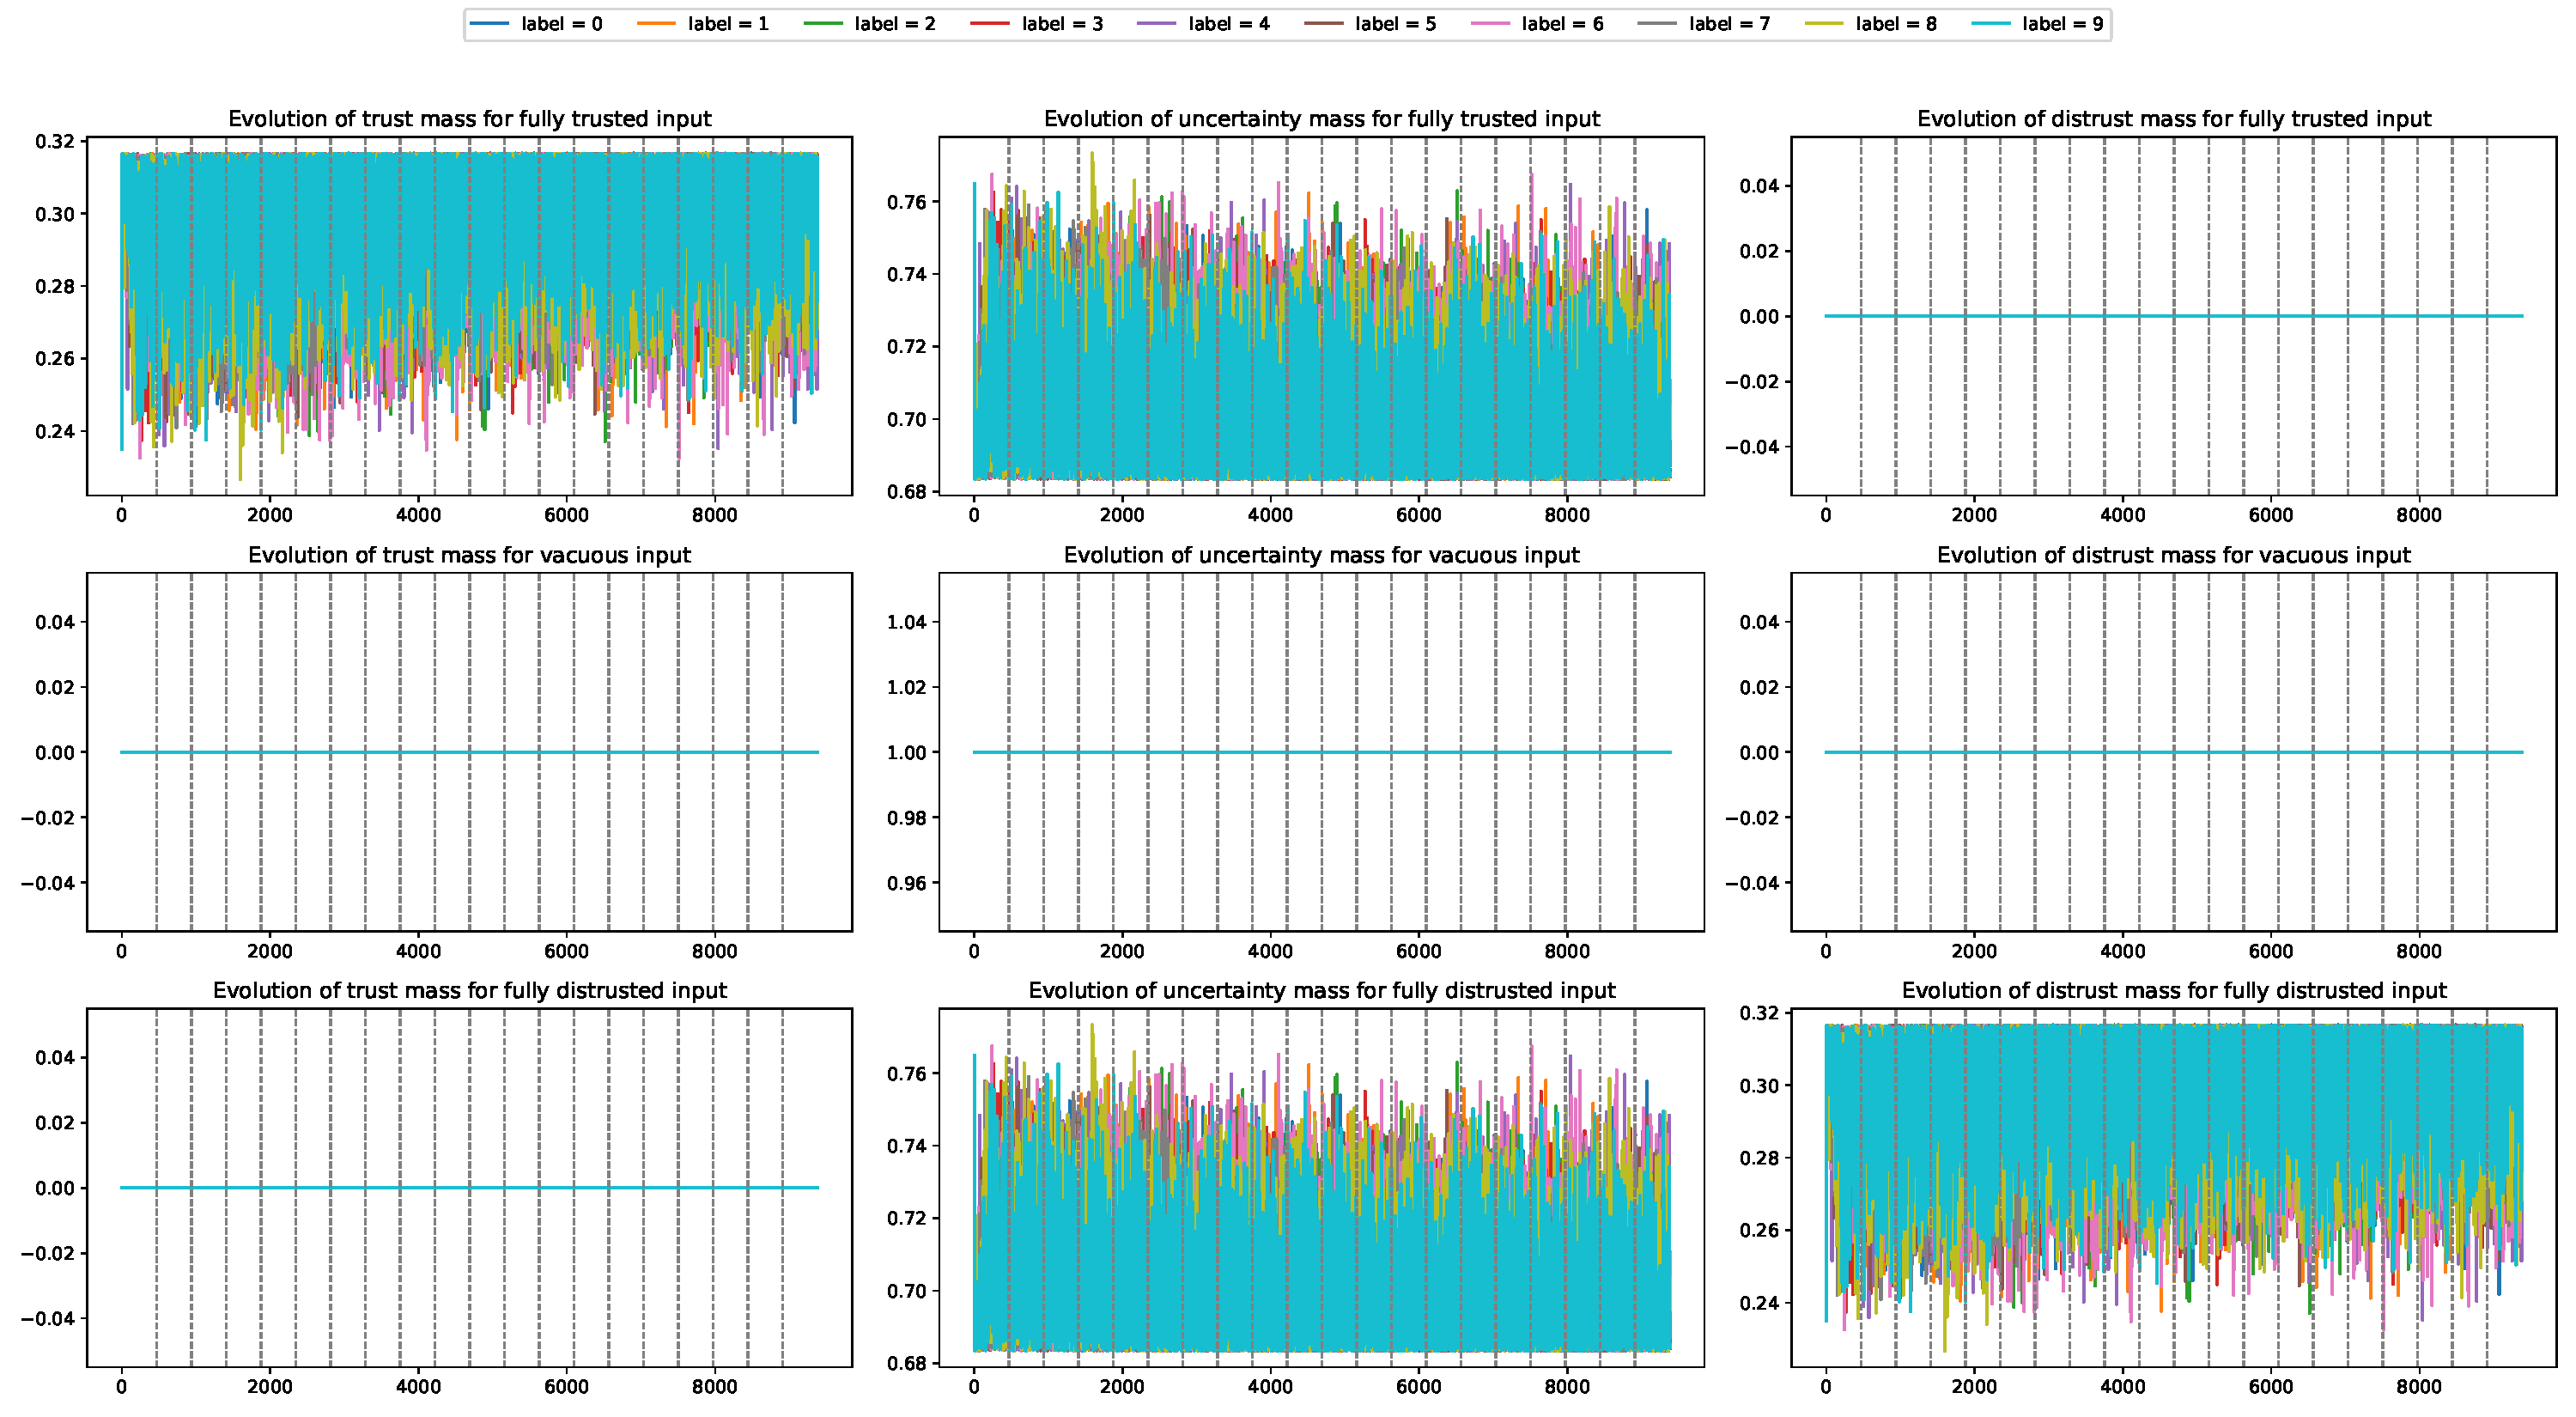
\includegraphics[width=\textwidth]{plots_v2/MNIST/architecture/plot_ptas-16-v-v.pdf}
  \caption{16 Hidden neurons}
\end{figure}
\begin{figure}[H]
  \centering
  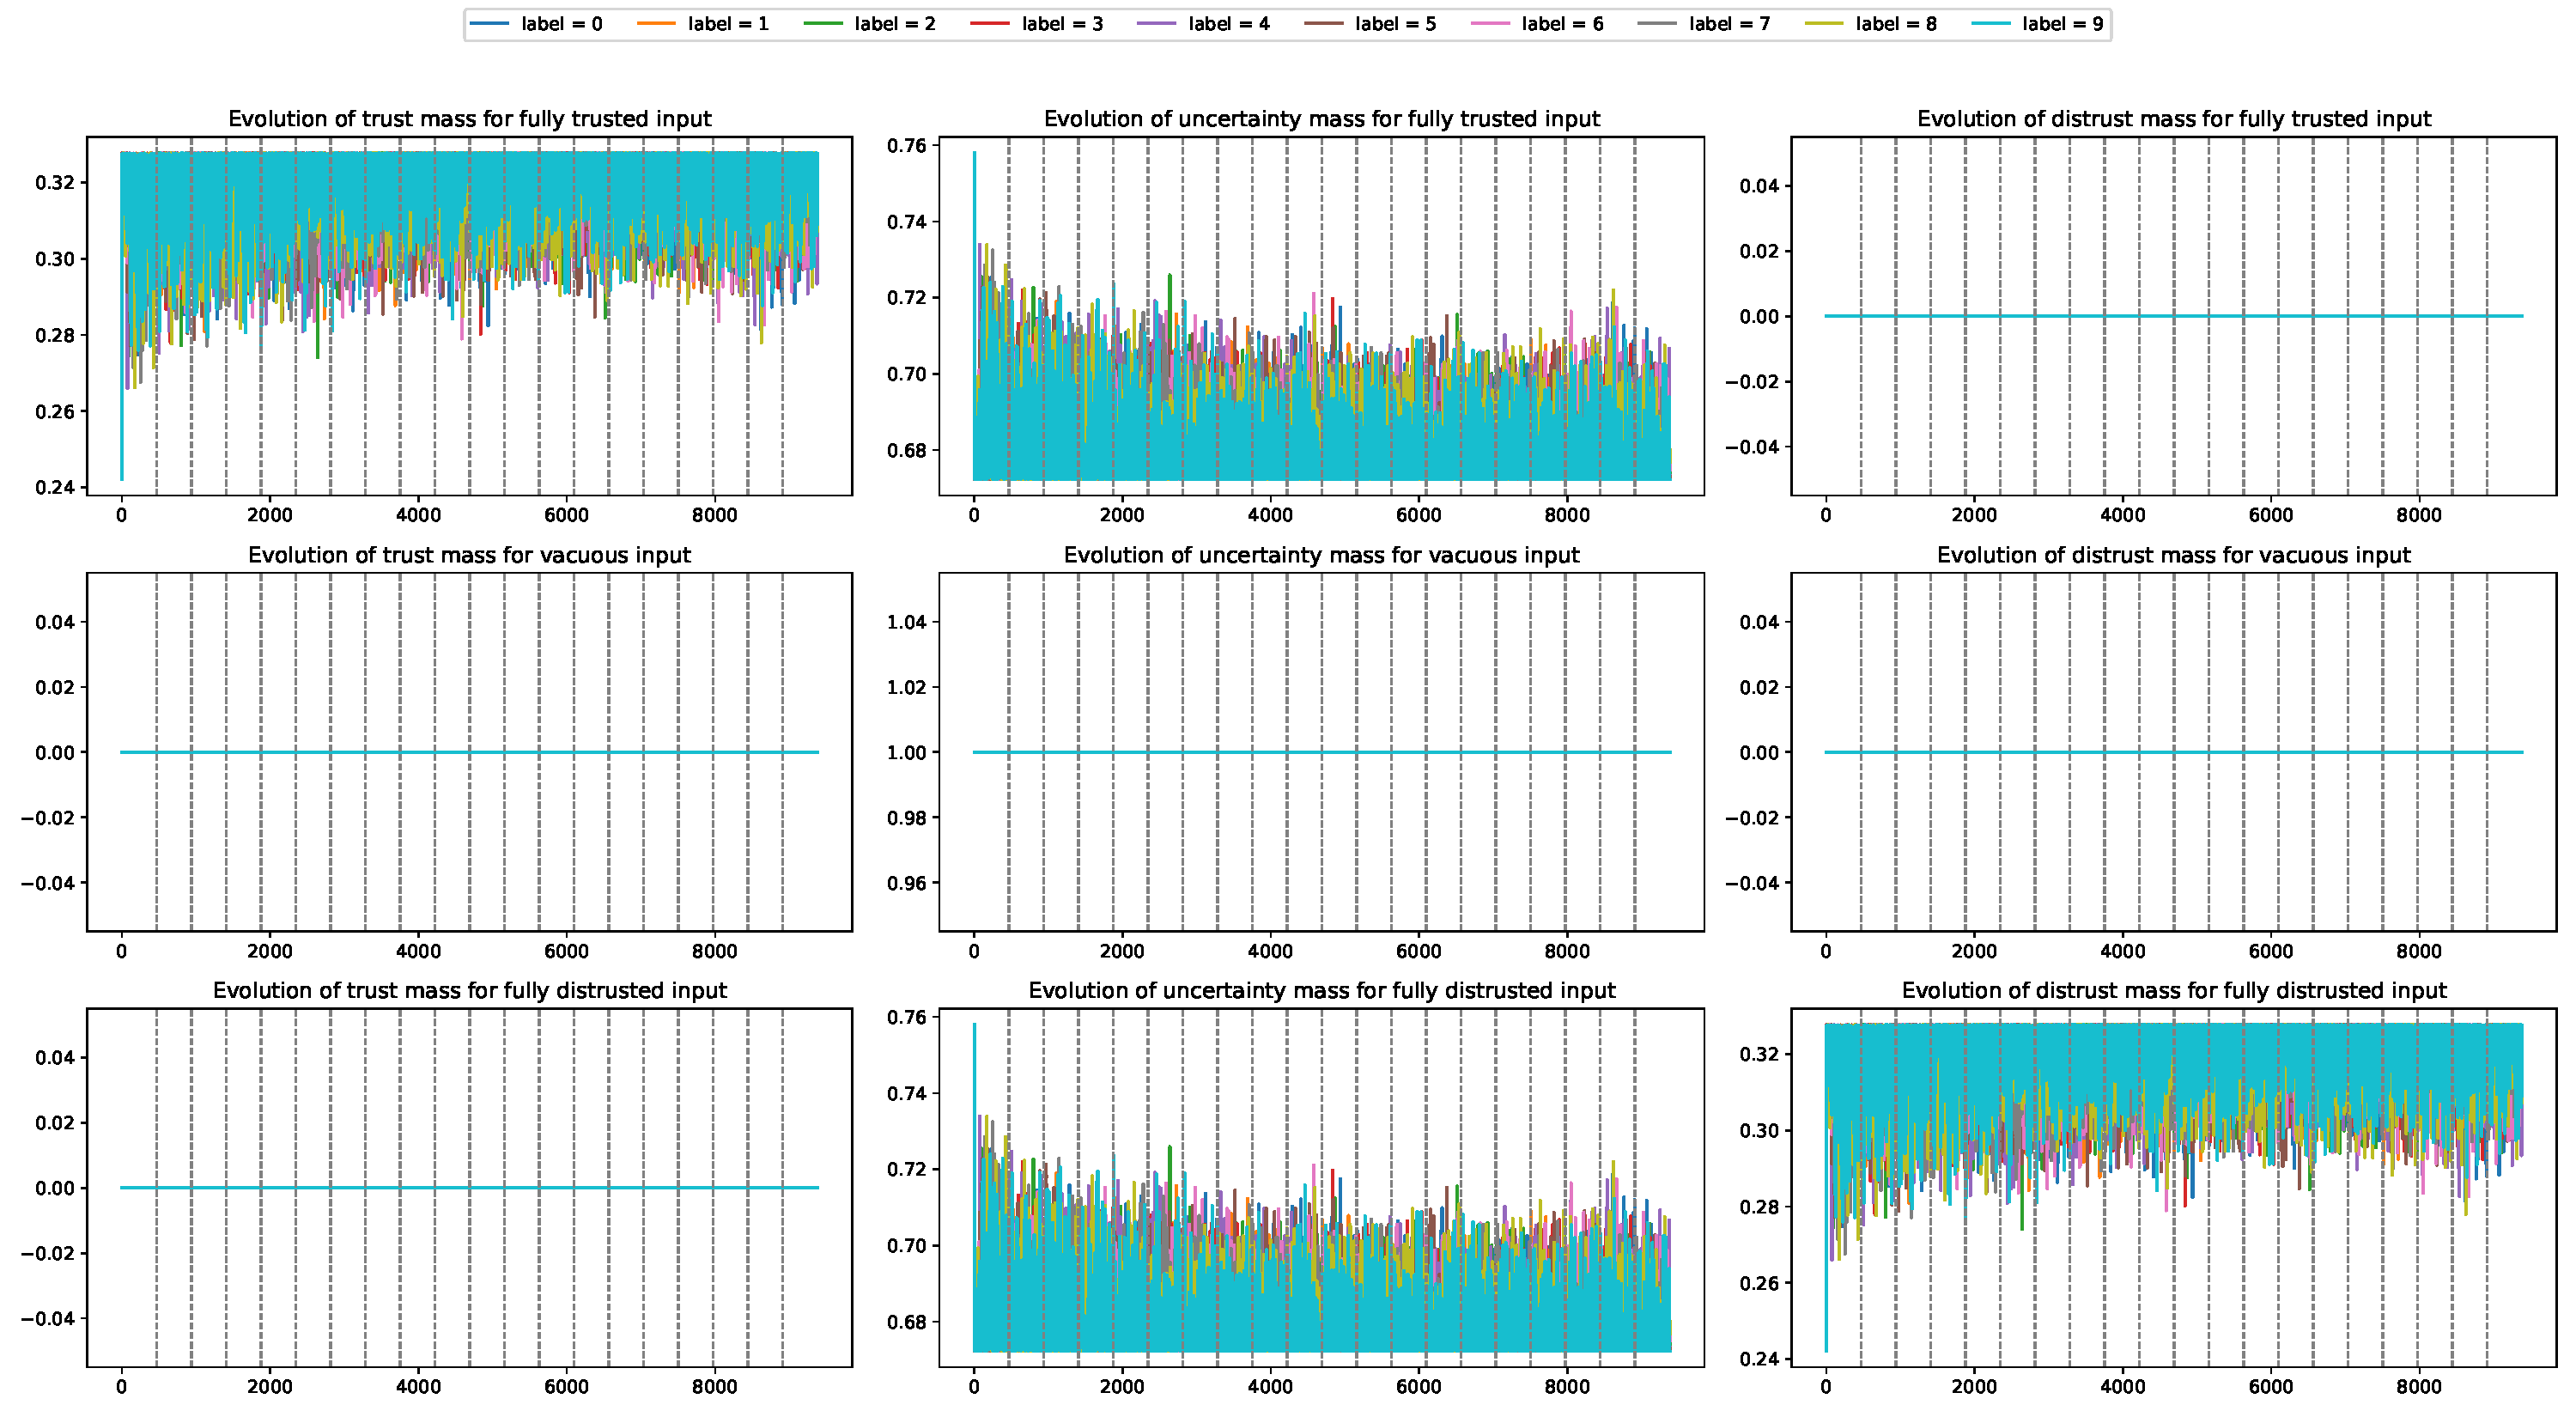
\includegraphics[width=\textwidth]{plots_v2/MNIST/architecture/plot_ptas-32-v-v.pdf}
  \caption{32 Hidden neurons}
\end{figure}
\begin{figure}[H]
  \centering
  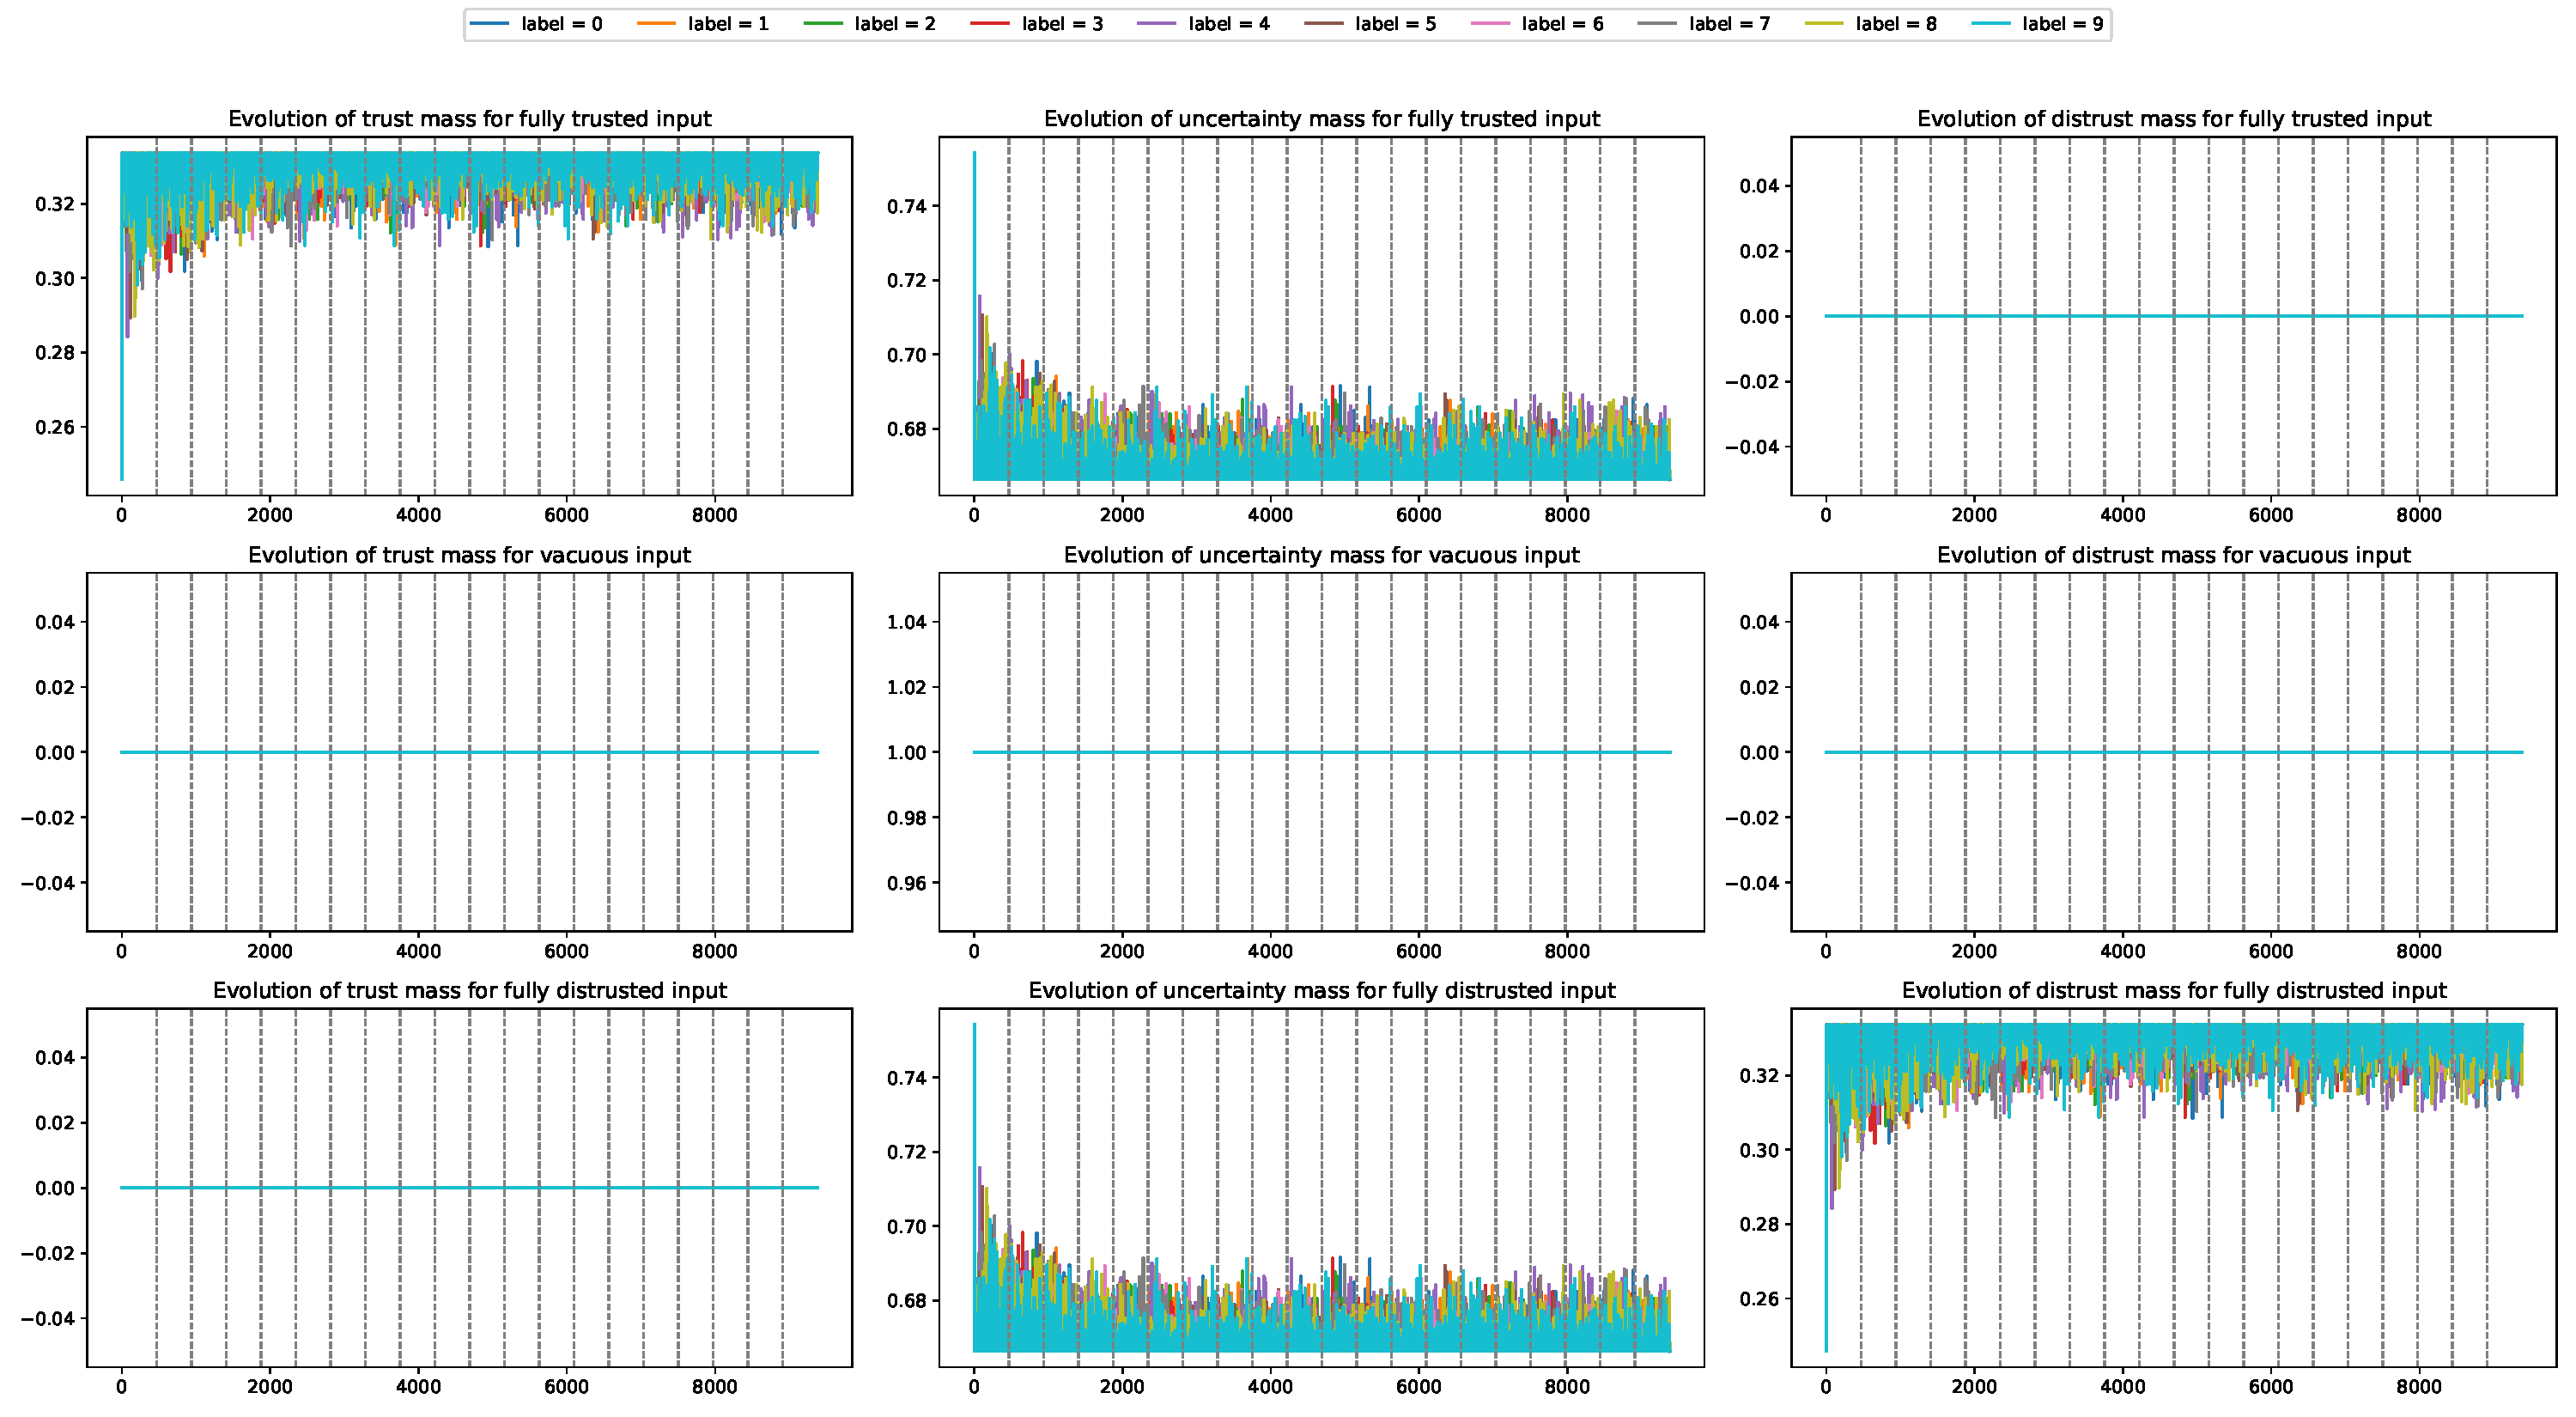
\includegraphics[width=\textwidth]{plots_v2/MNIST/architecture/plot_ptas-64-v-v.pdf}
  \caption{64 Hidden neurons}
\end{figure}
\begin{figure}[H]
  \centering
  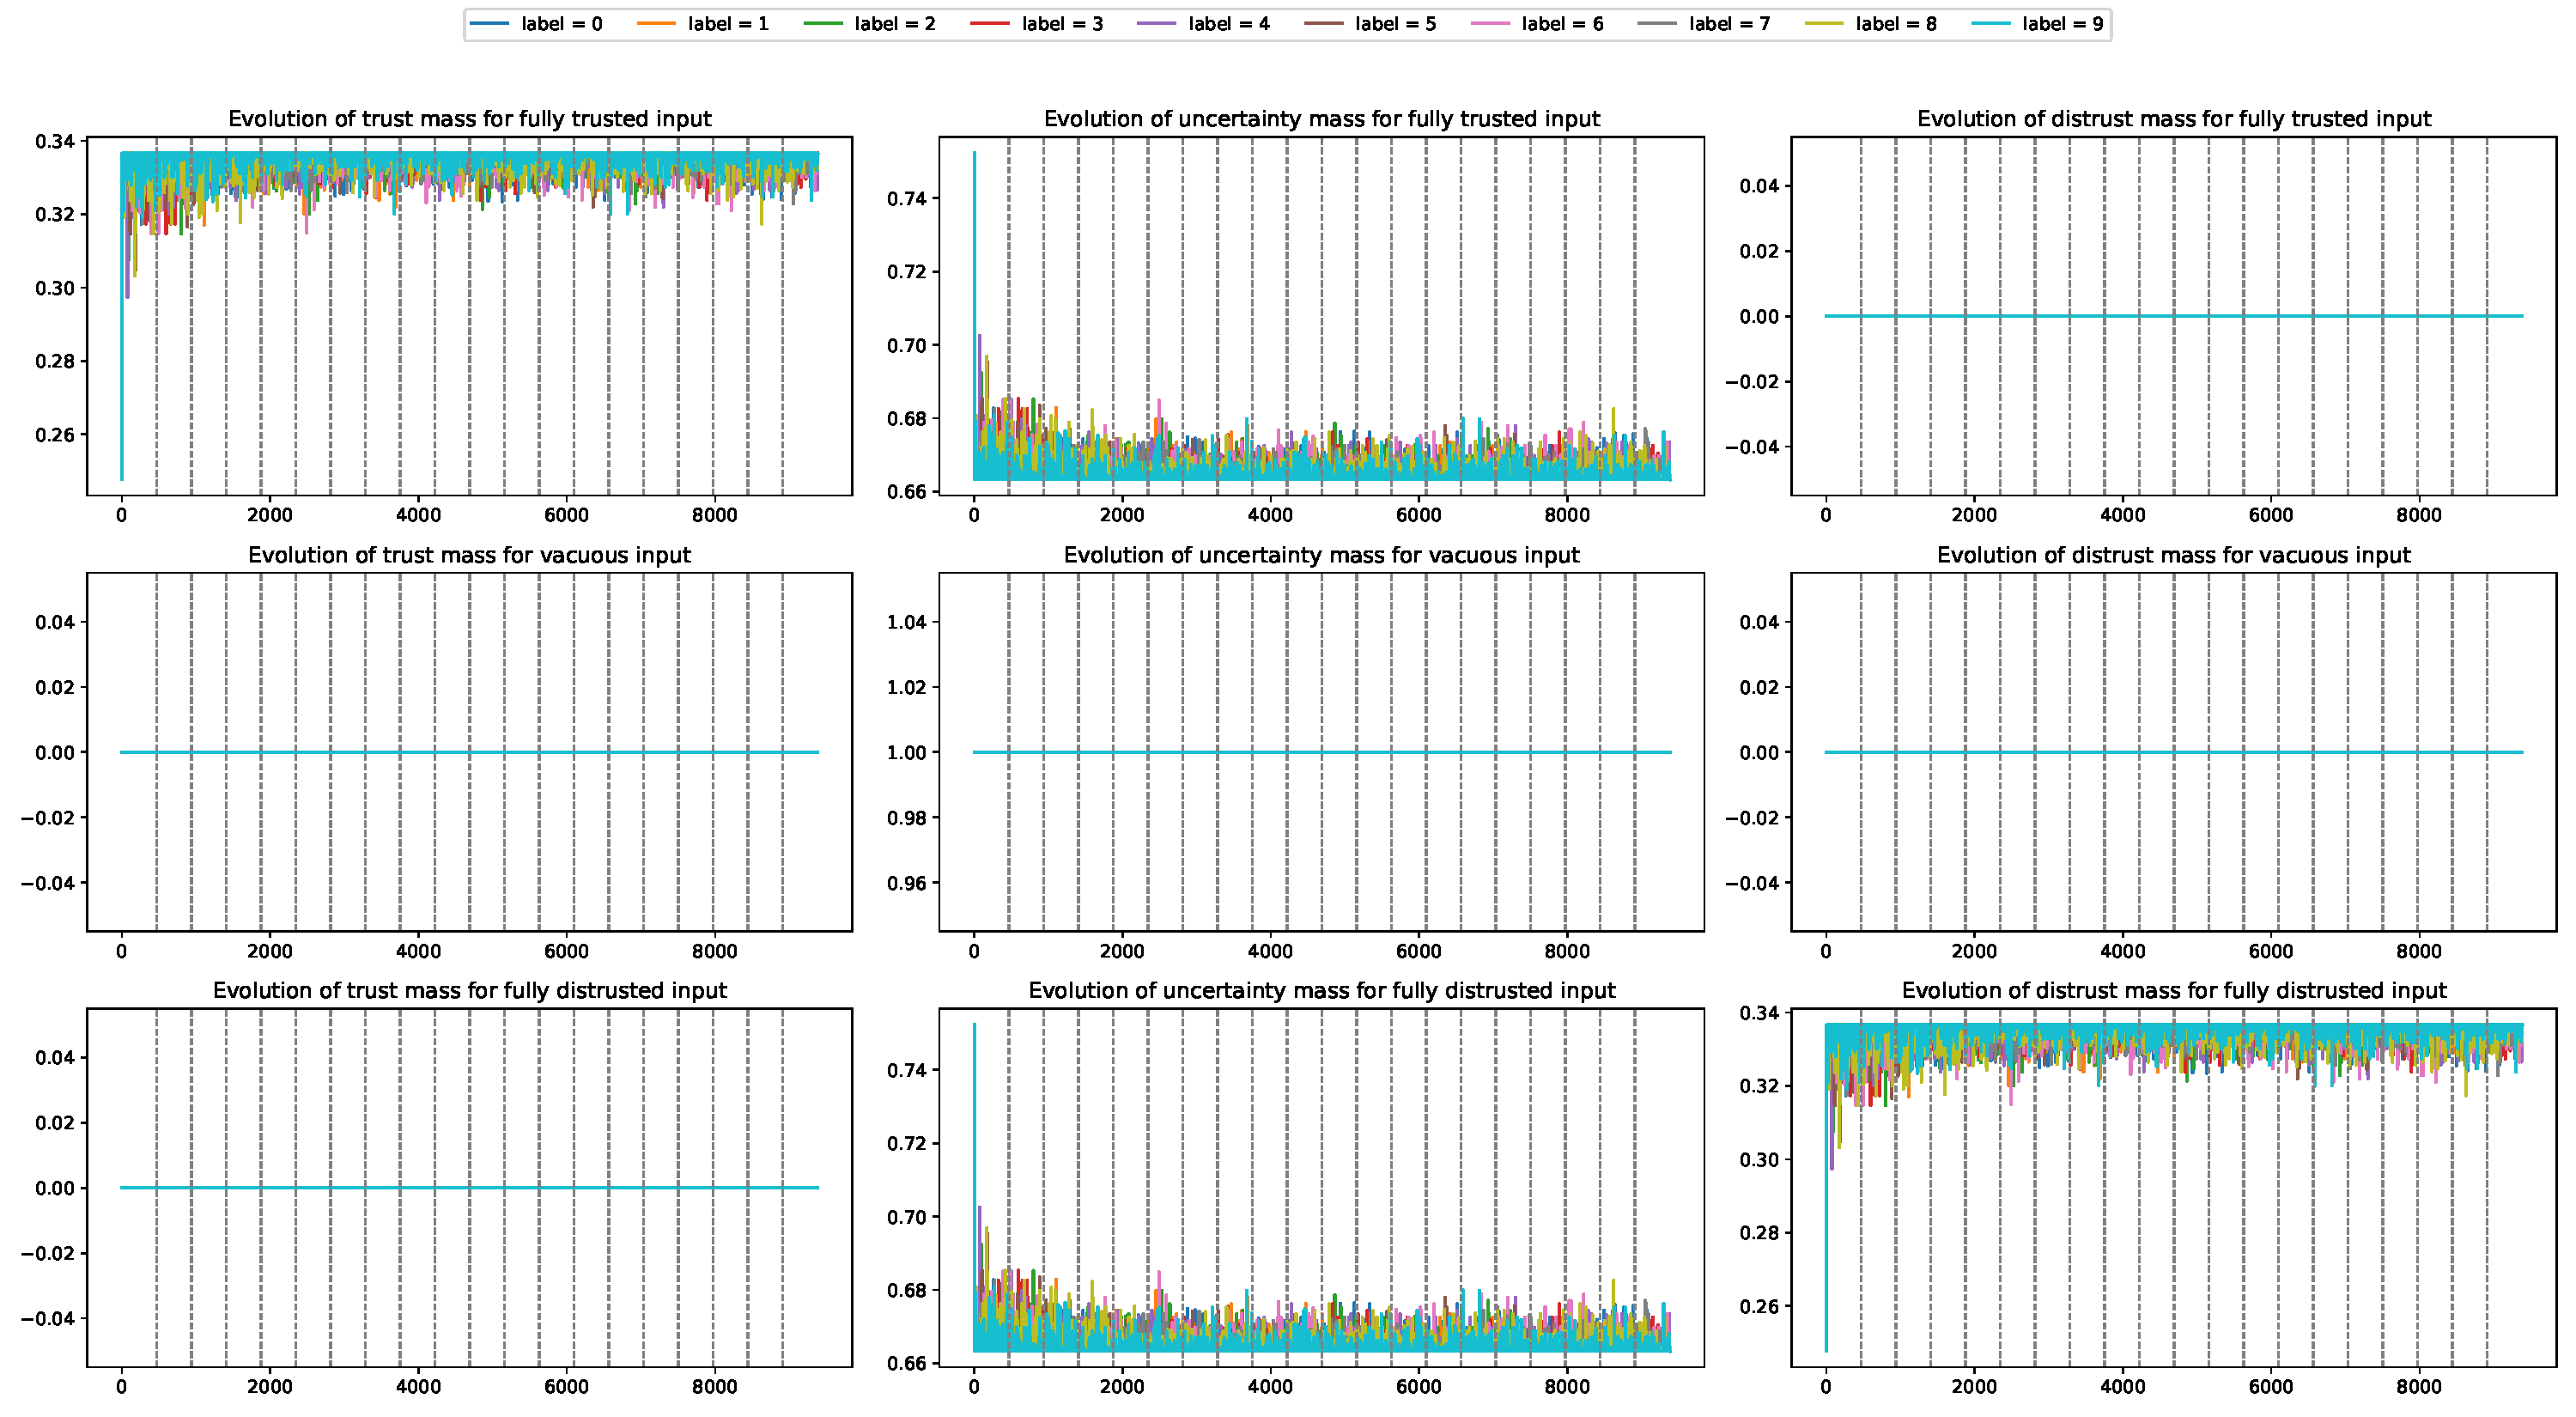
\includegraphics[width=\textwidth]{plots_v2/MNIST/architecture/plot_ptas-128-v-v.pdf}
  \caption{128 Hidden neurons}
\end{figure}
\begin{figure}[H]
  \centering
  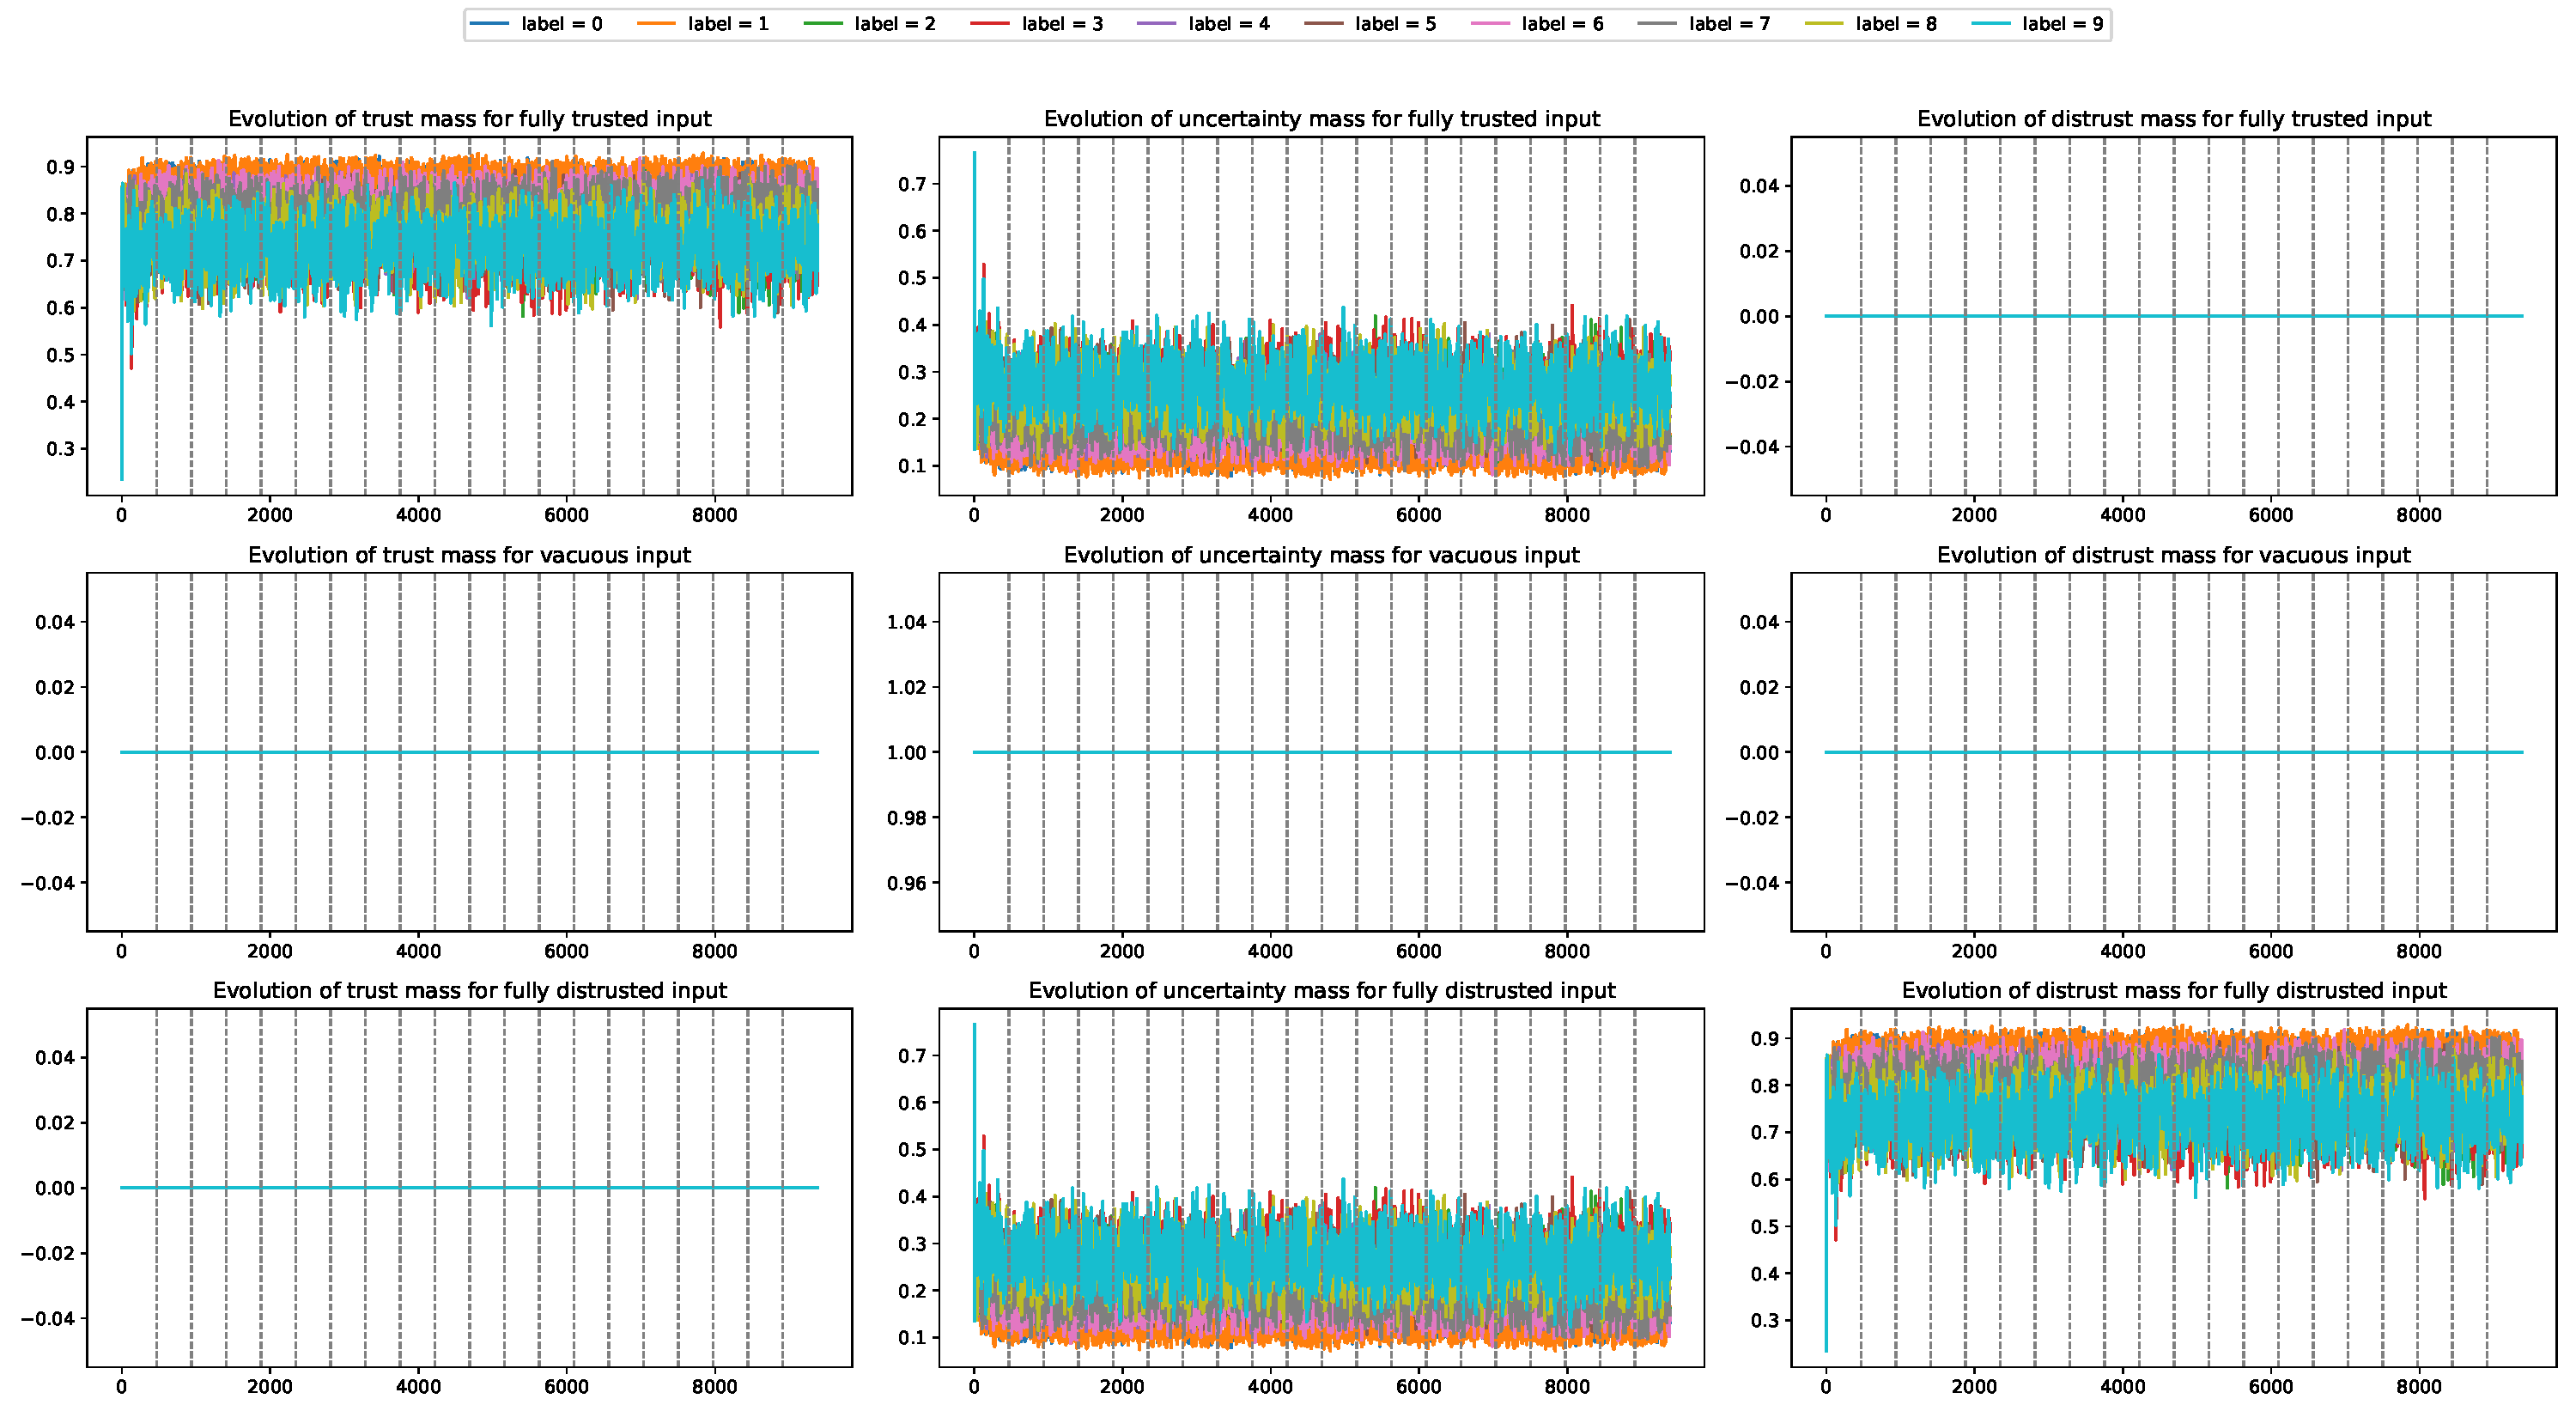
\includegraphics[width=\textwidth]{plots_v2/MNIST/architecture/plot_ptas-16-t-t.pdf}
  \caption{16 Hidden neurons with Fully Trusted Assessment}
\end{figure}

\subsection{MNIST poisoned 128 hidden neurons (\cref{exp:3})}\label{sec:resmnistpois}
\begin{figure}[H]
  \centering
  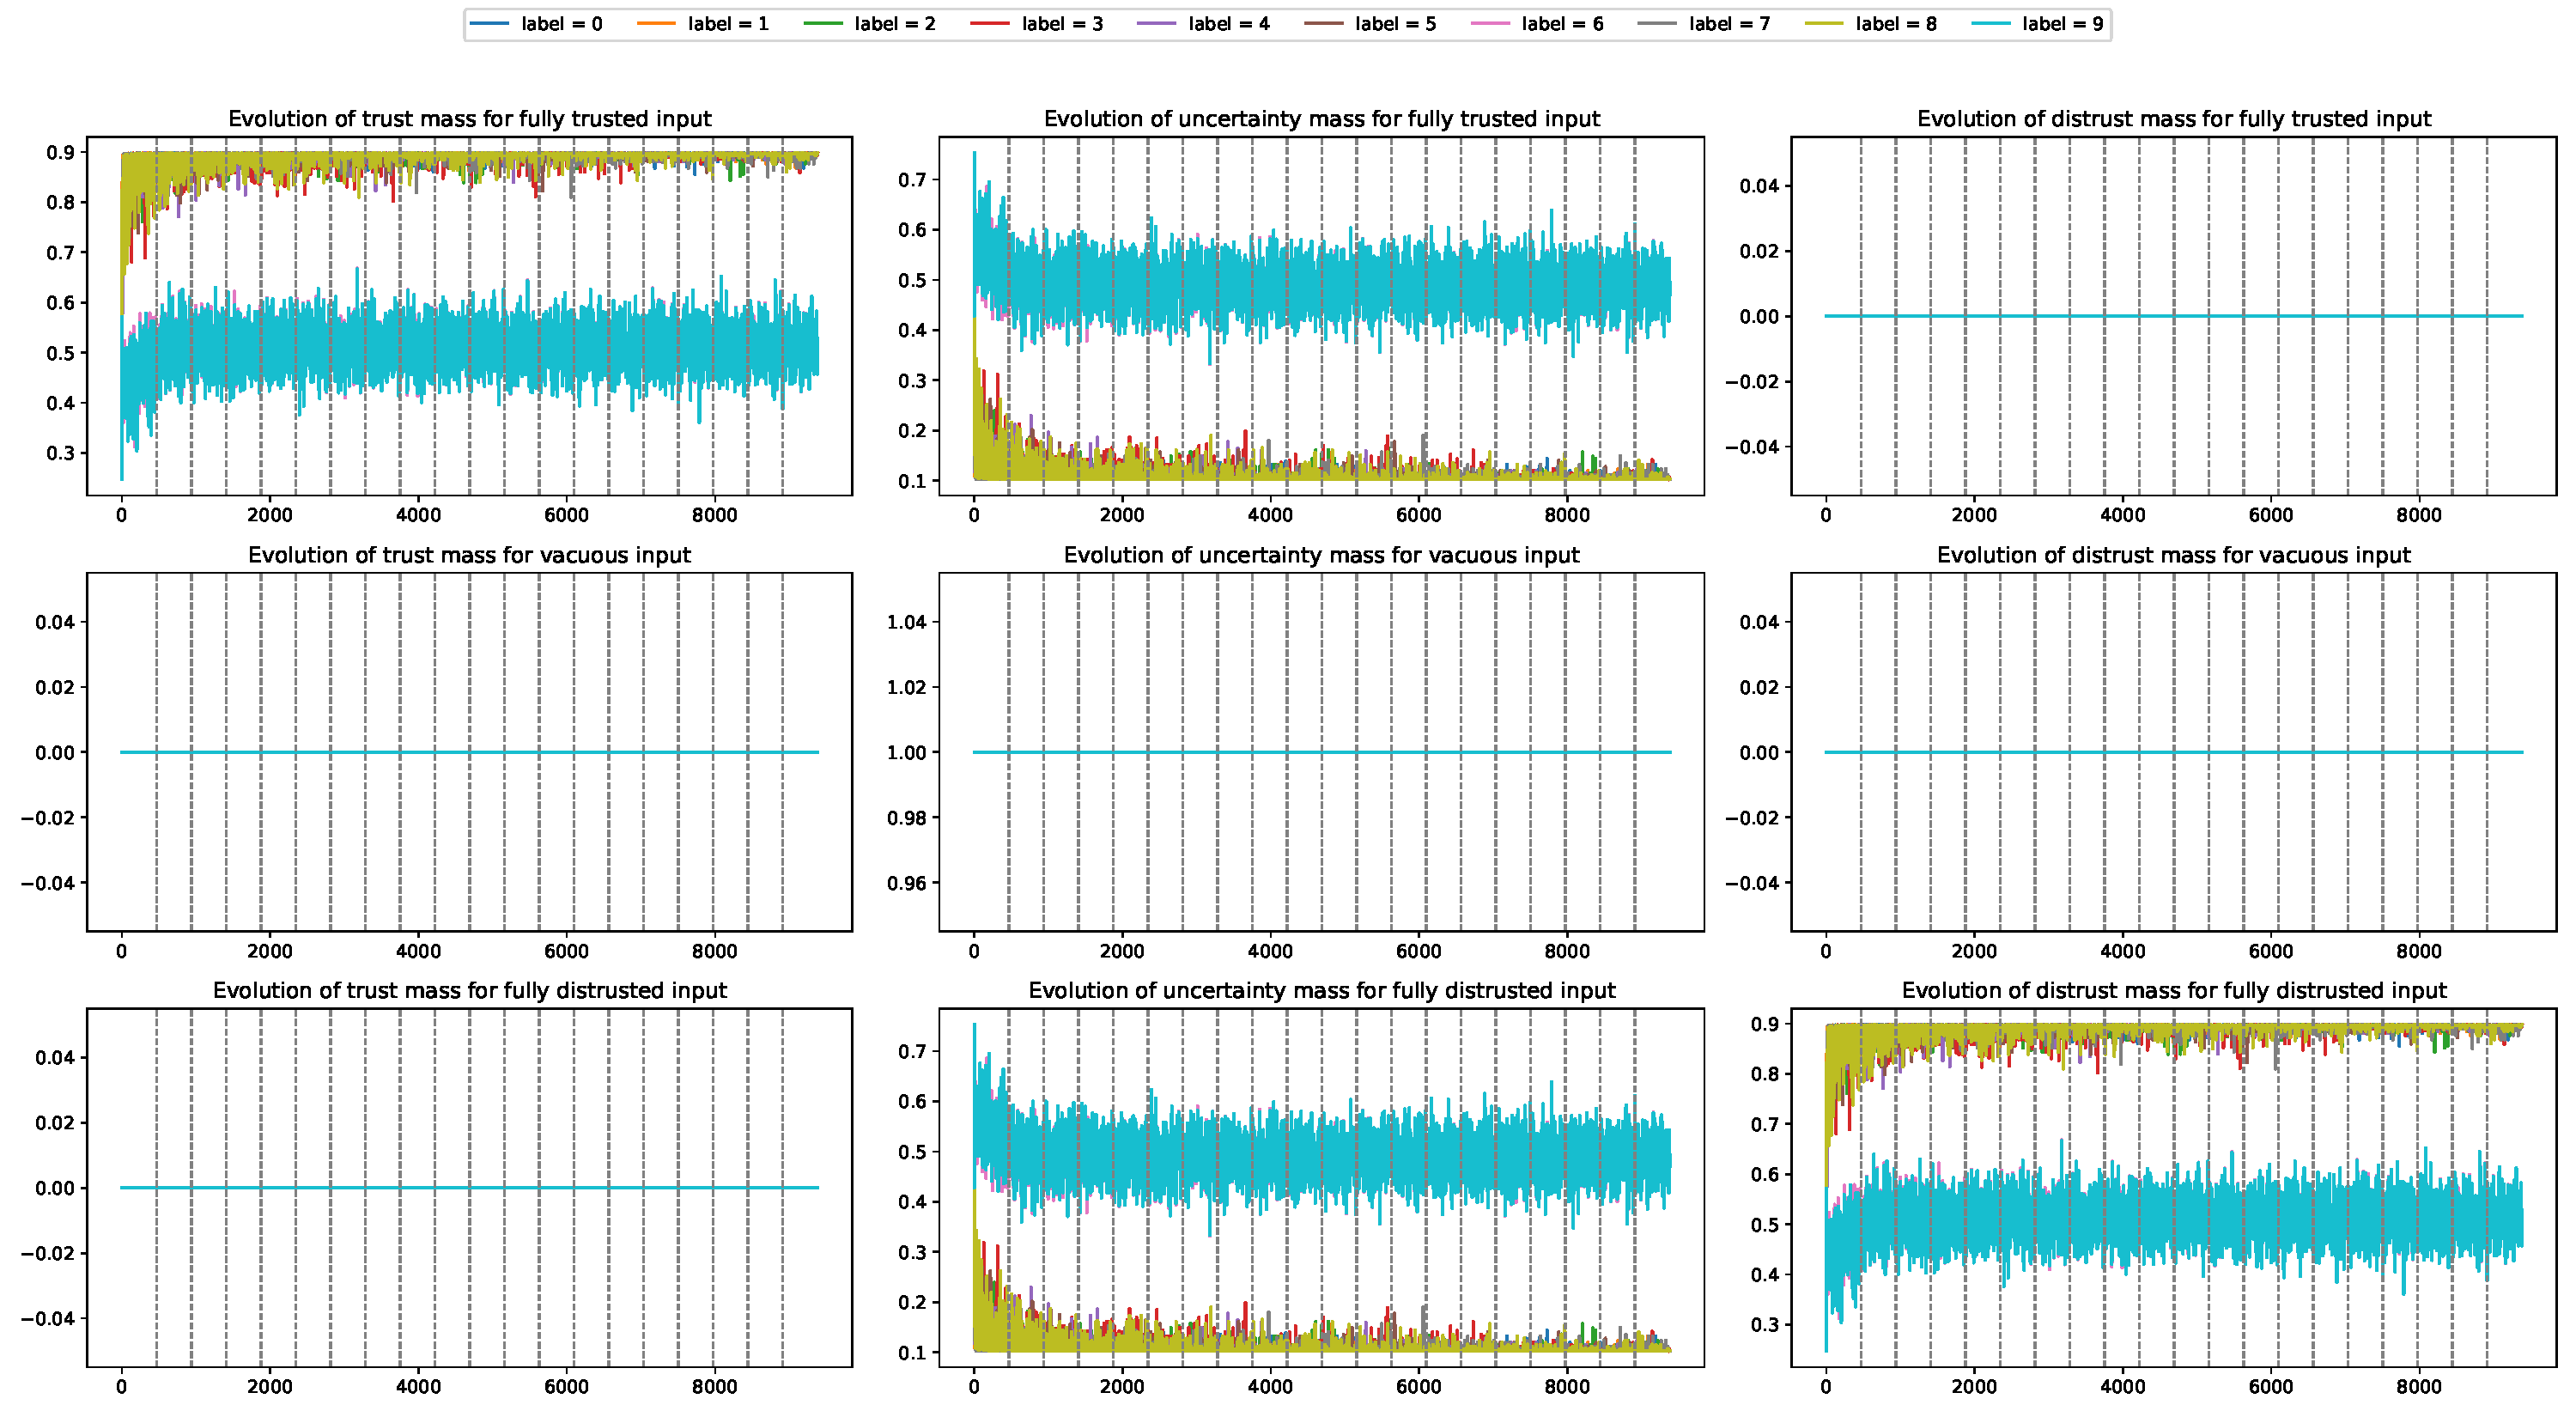
\includegraphics[width=\textwidth]{plots_v2/MNIST/poisoned/plot_ptas-128-t-t-ps1.pdf}
  \caption{1 pixel}
\end{figure}
\begin{figure}[H]
  \centering
  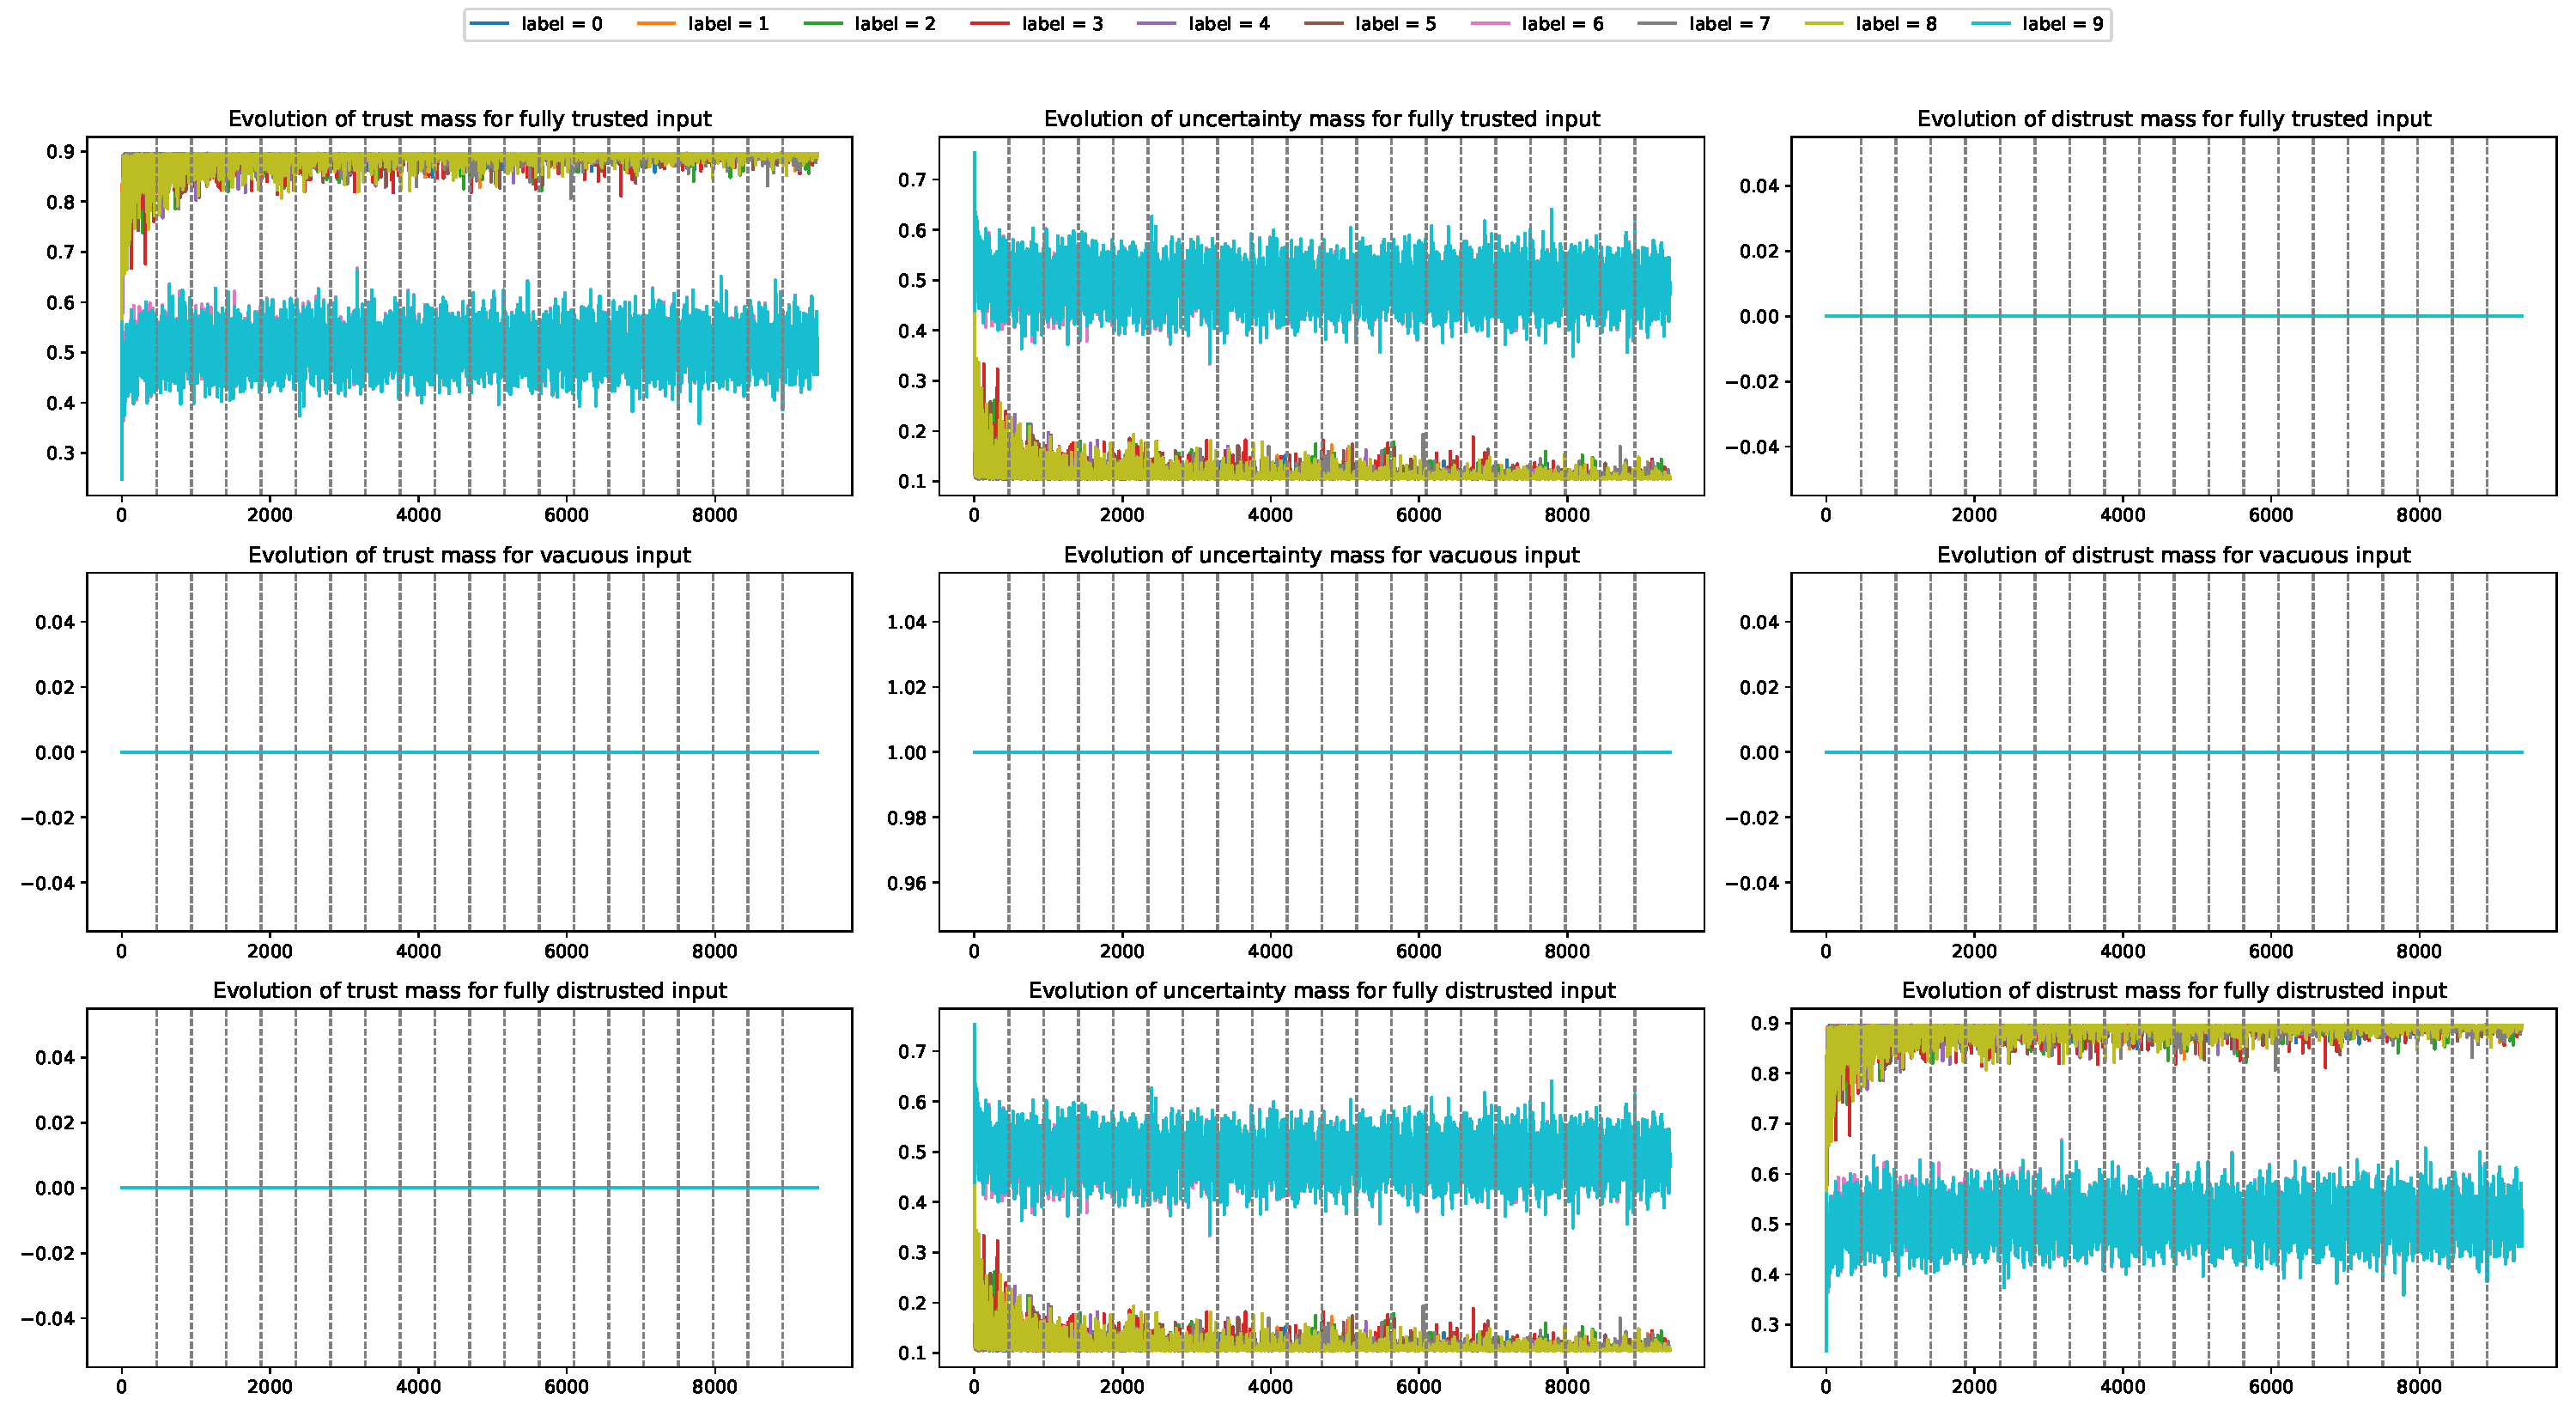
\includegraphics[width=\textwidth]{plots_v2/MNIST/poisoned/plot_ptas-128-t-t-ps4.pdf}
  \caption{4×4 pixels}
\end{figure}
\begin{figure}[H]
  \centering
  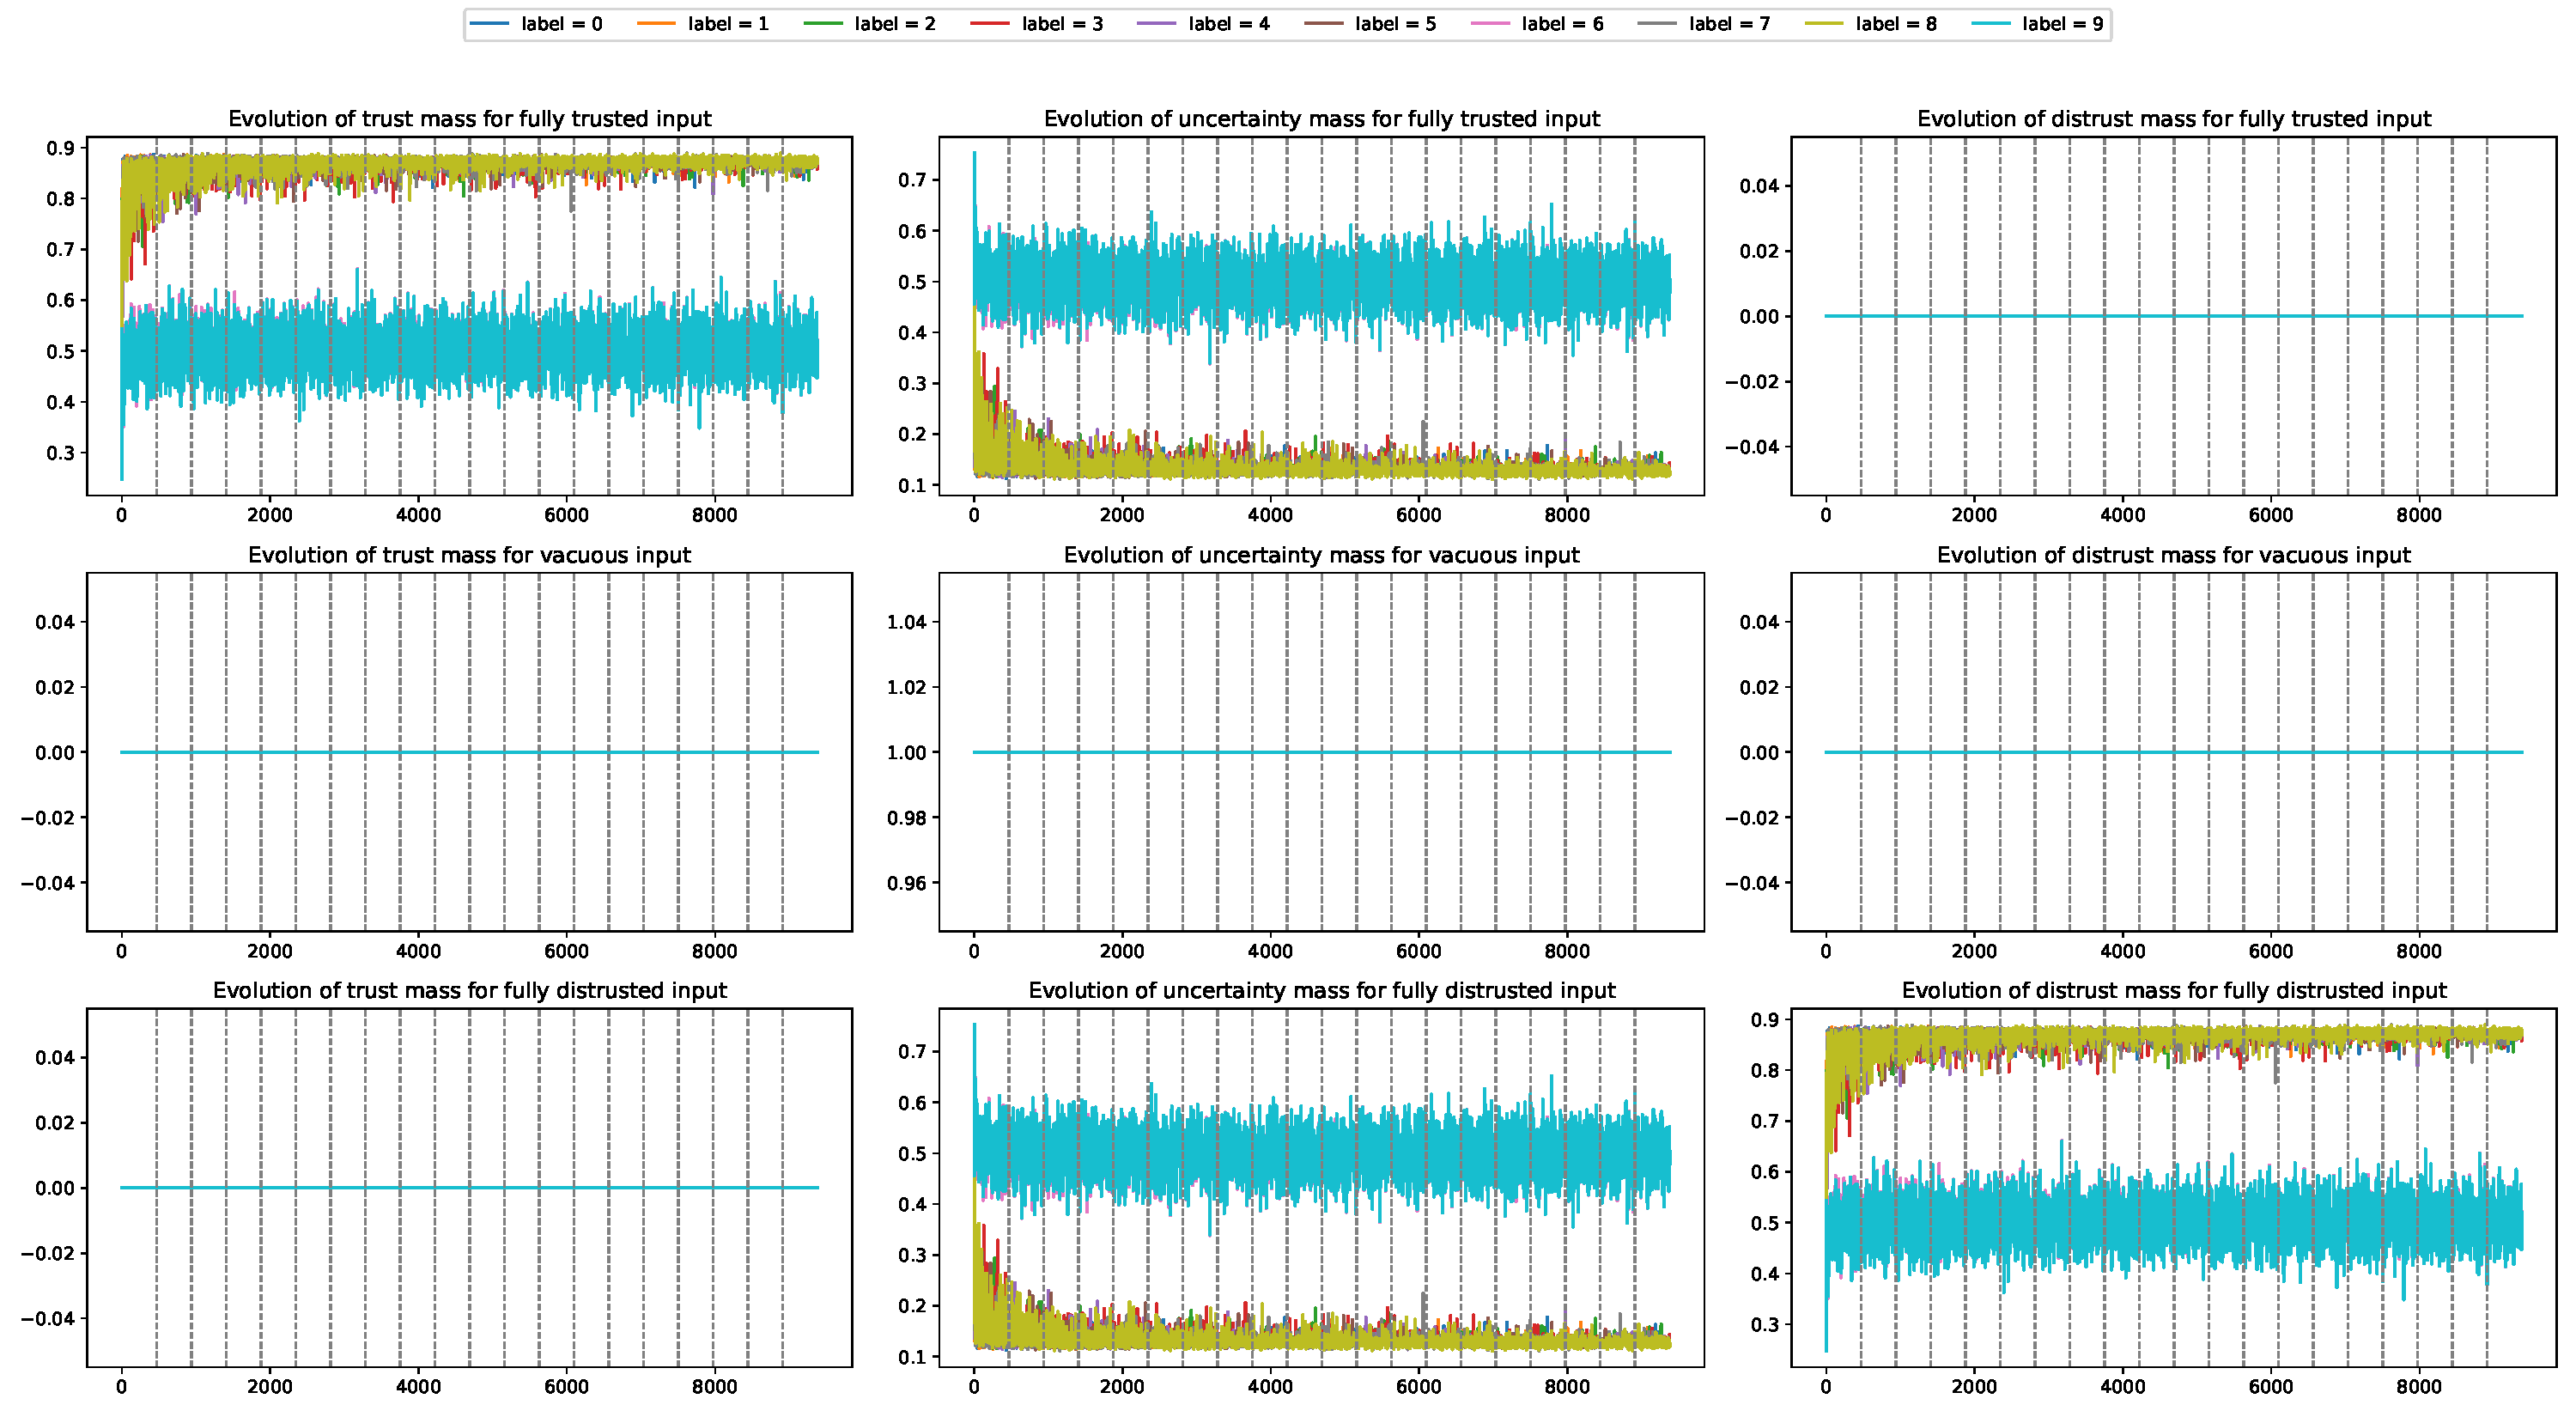
\includegraphics[width=\textwidth]{plots_v2/MNIST/poisoned/plot_ptas-128-t-t-ps10.pdf}
  \caption{10×10 pixels}
\end{figure}
\begin{figure}[H]
  \centering
  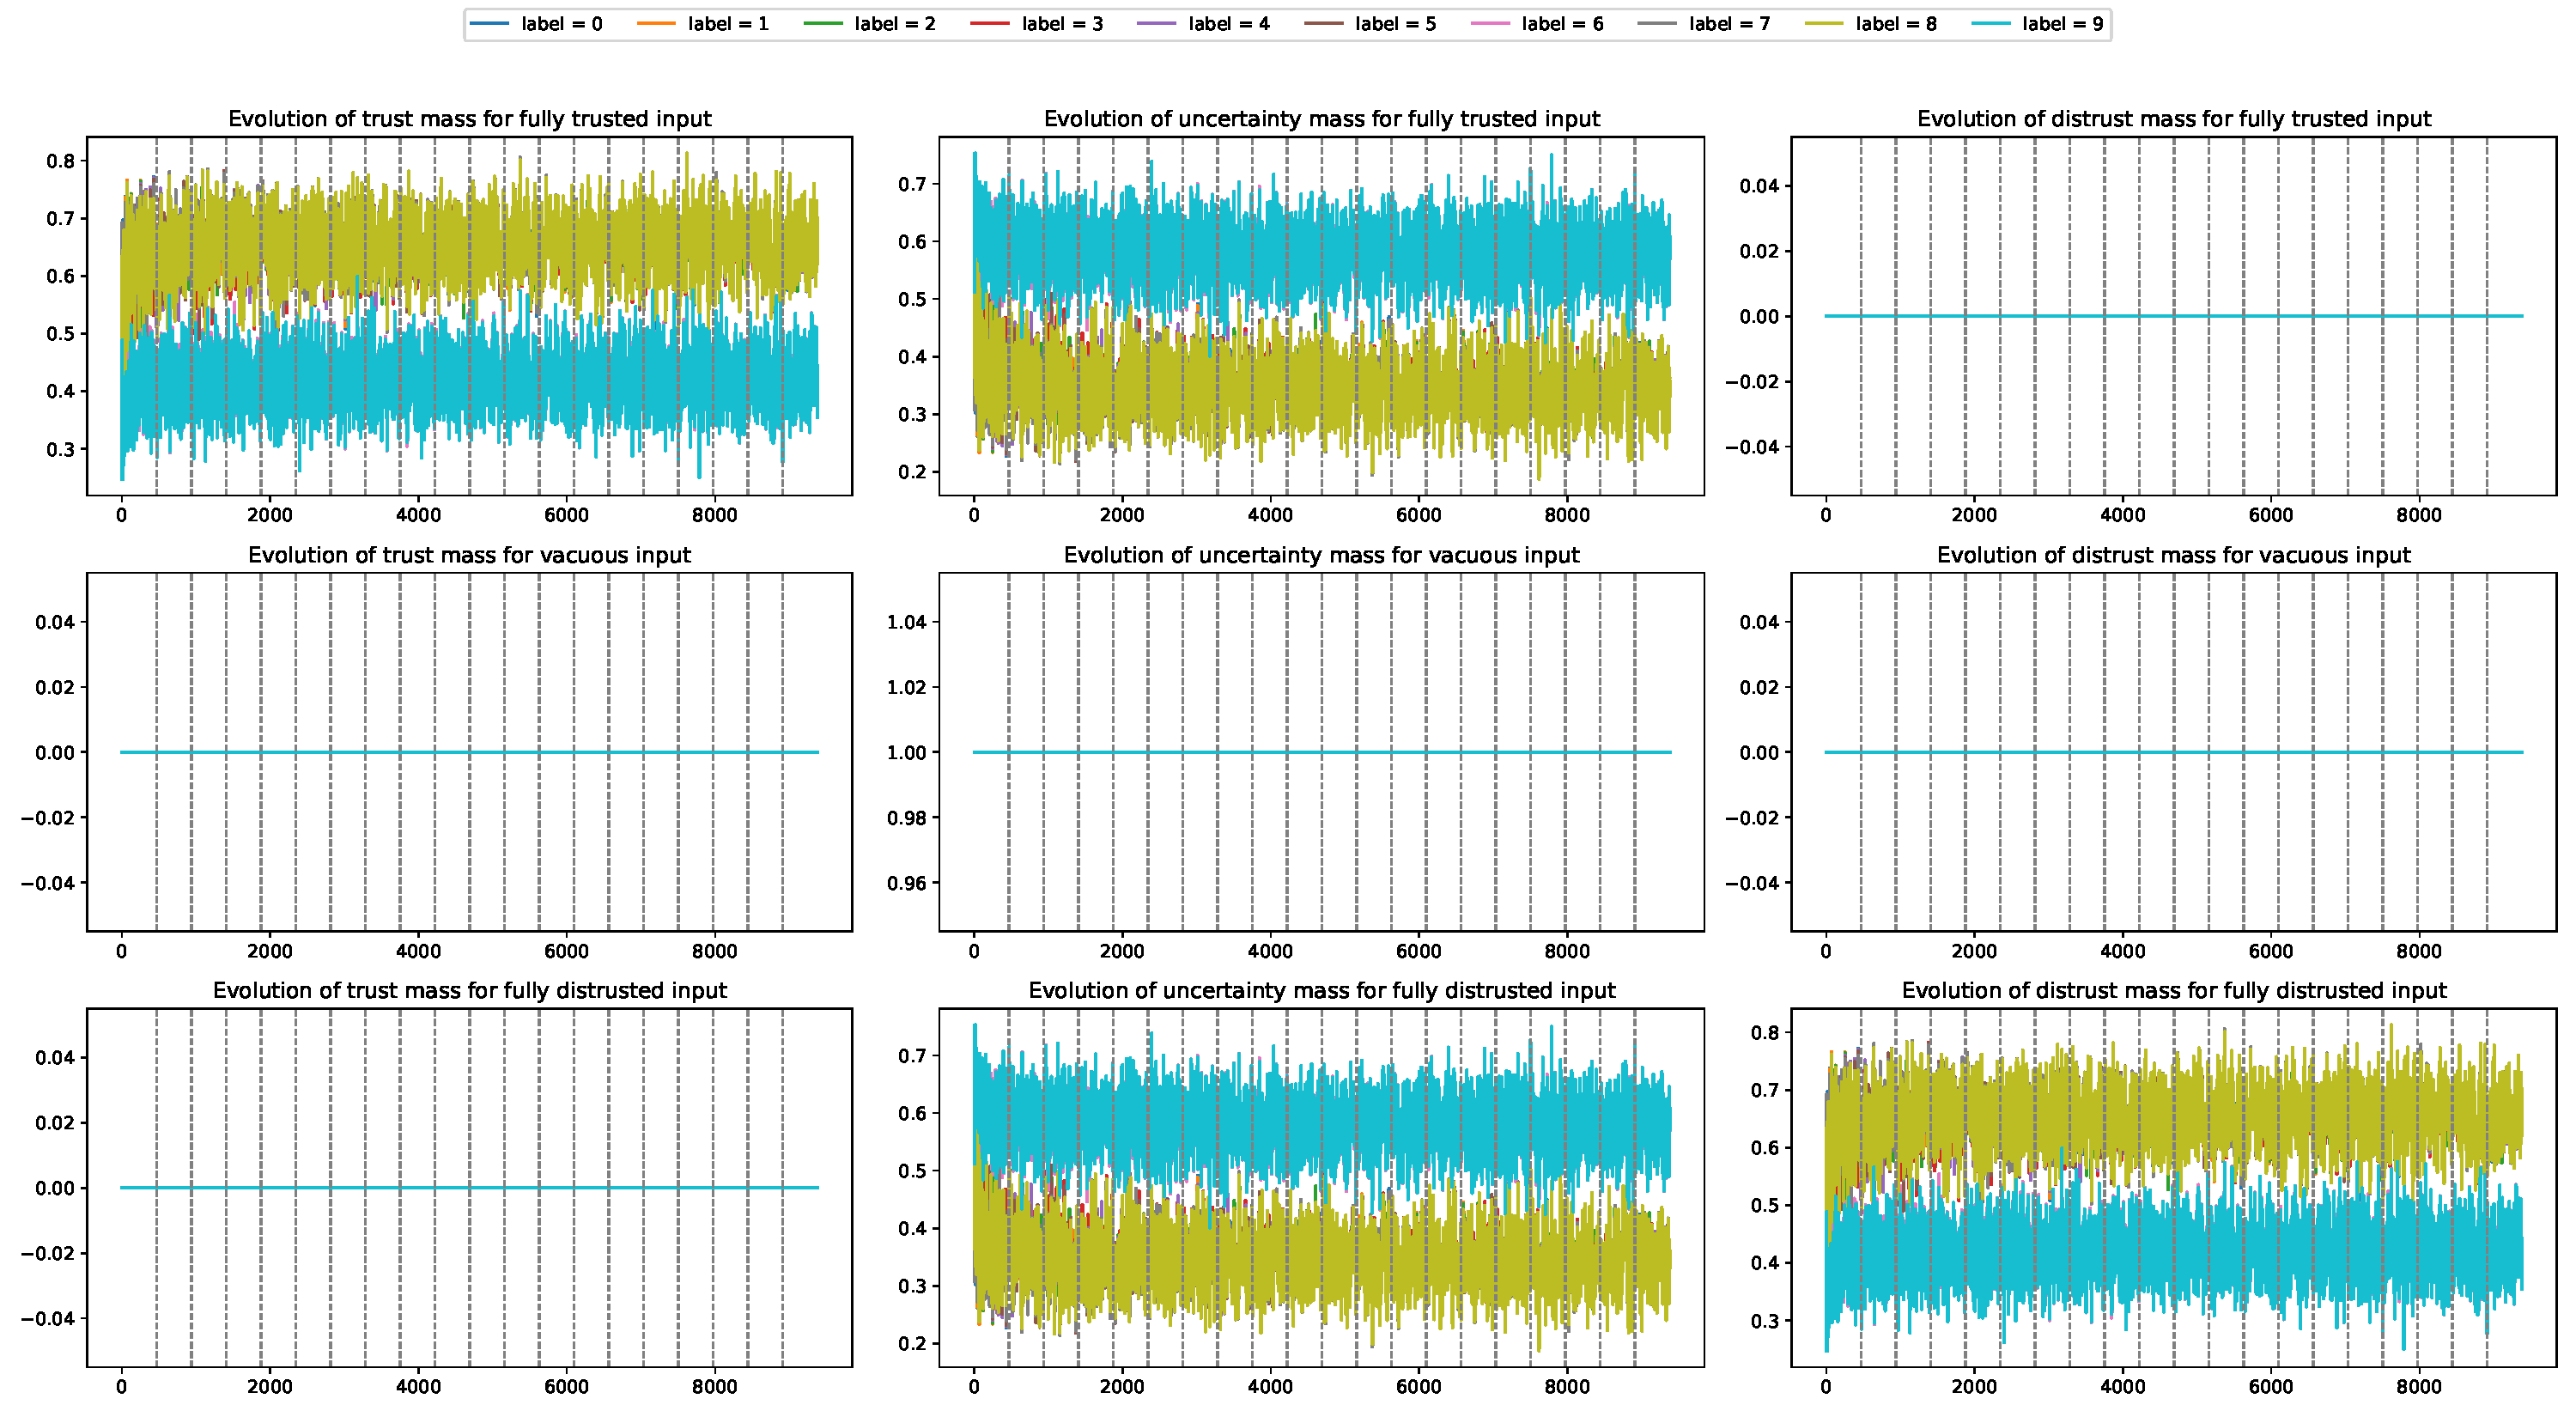
\includegraphics[width=\textwidth]{plots_v2/MNIST/poisoned/plot_ptas-128-t-t-ps27.pdf}
  \caption{27×27 pixels}
\end{figure}
\subsection{Plots for the Comparative Trust Evaluation (\cref{exp:4})}\label{sec:resexp4}
\begin{figure}[H]
  \centering
  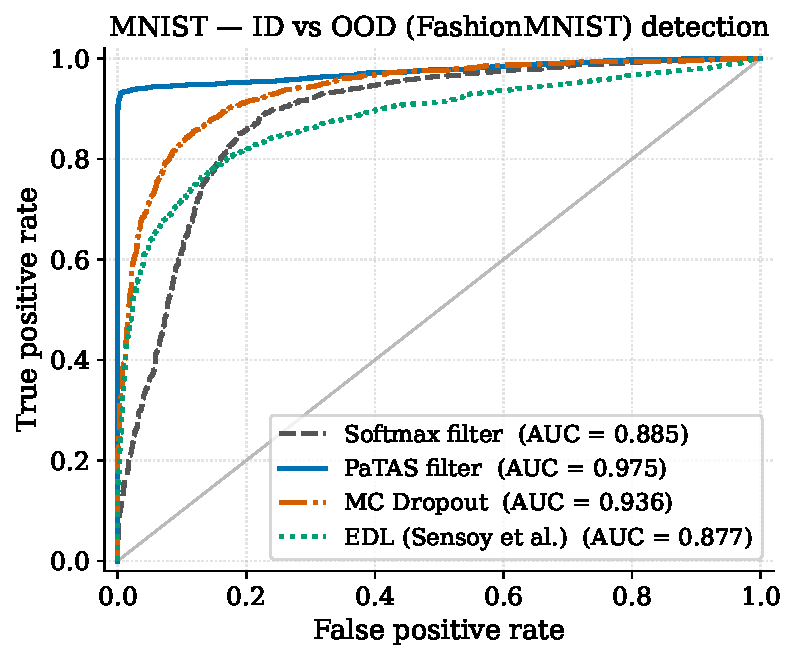
\includegraphics[width=0.62\textwidth]{plots_v2/exp4/roc_ood_mnist.pdf}
  \caption{Out-of-distribution detection ROC (MNIST in-distribution vs.\ Fashion-MNIST OOD): each method's own score as the discriminator. Curves and legend AUC values are from a single representative evaluation seed; \cref{tab:comparative} reports mean $\pm$ std over three seeds.}
\end{figure}
\begin{figure}[H]
  \centering
  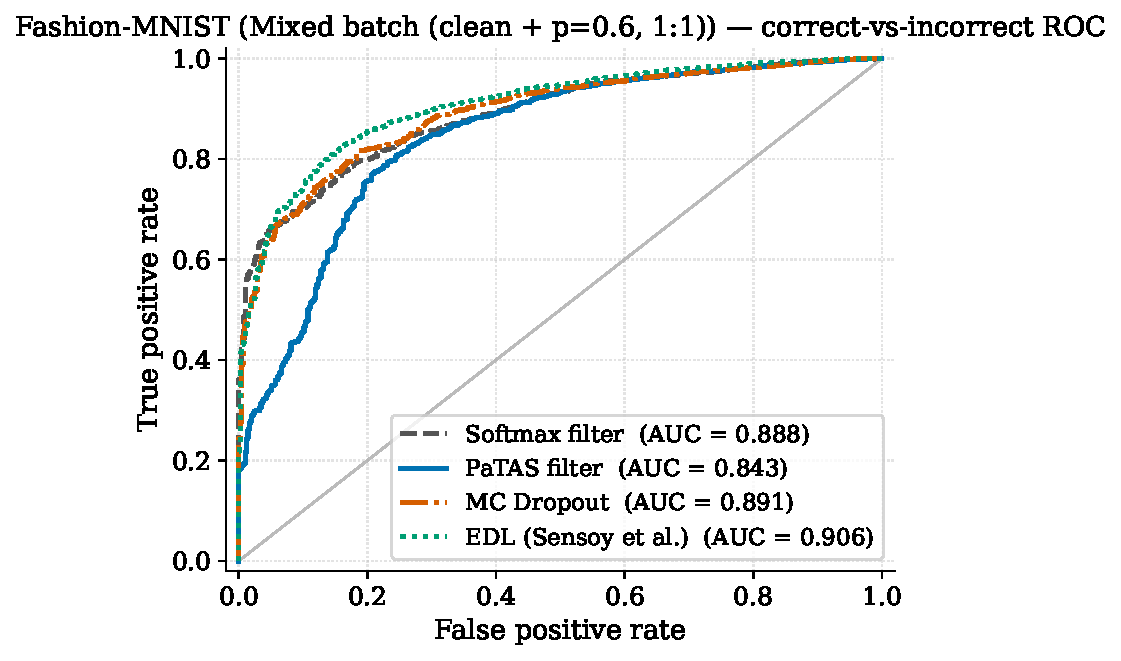
\includegraphics[width=0.62\textwidth]{plots_v2/exp4/roc_mixed_fashion.pdf}
  \caption{Correct-vs-incorrect ROC on the Fashion-MNIST mixed batch (clean + corrupted inputs pooled 1:1), single representative evaluation seed.}
\end{figure}
\begin{figure}[H]
  \centering
  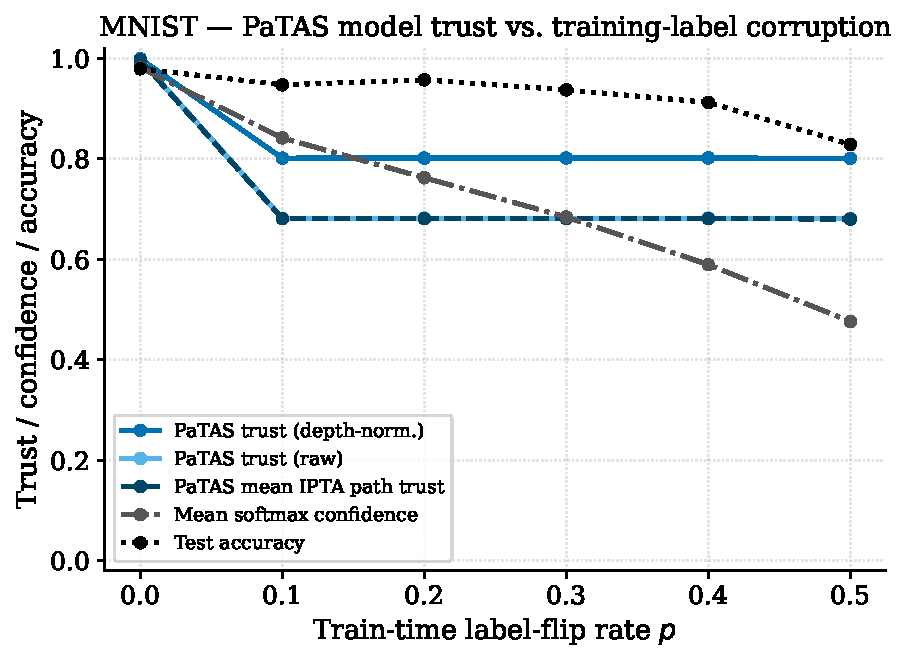
\includegraphics[width=0.62\textwidth]{plots_v2/exp4/model_trust_vs_labelnoise.pdf}
  \caption{Training-quality audit (\cref{tab:audit}): PaTAS model-side trust, mean softmax confidence, and test accuracy as functions of the train-time label-flip rate $p$. The depth-normalized curve rescales the committed mass $b+d$ of the aggregated opinion to $(b+d)^{1/L}$, with $L$ the number of trust-propagation layers, making trust comparable across network depths. Trust drops as a tripwire at any non-zero rate without using test data; confidence tracks severity but requires a clean labelled test set.}
\end{figure}
